% MSc dissertation example file, February 2022
%
% Leave one of the documentclass lines uncommented to match your degree.
% You may remove the logo option if it causes problems.
% Do not change any other options.
% \documentclass[logo,msc,adi]{infthesis}         % Adv Design Inf
% \documentclass[logo,msc,ai]{infthesis}          % AI
% \documentclass[logo,msc,cogsci]{infthesis}      % Cognitive Sci
% \documentclass[logo,msc,cs]{infthesis}          % Computer Sci
% \documentclass[logo,msc,cyber]{infthesis}       % Cyber Sec
% \documentclass[logo,msc,datasci]{infthesis}     % Data Sci
% \documentclass[logo,msc,di]{infthesis}          % Design Inf
\documentclass[logo,msc,dsti]{style/infthesis}    % Data Sci TI
% \documentclass[logo,msc,inf]{infthesis}         % Informatics
% \documentclass[logo,msc]{infthesis}             % degree unspecified, do not change except to add your degree
%%%%%%%%%%%%%%%%%%%%%%%%
% Understand any problems and seek approval before assuming it's ok to remove ugcheck.
\usepackage{style/msccheck}

% Include any packages you need below, but don't include any that change the page
% layout or style of the dissertation. By including the ugcheck package above,
% you should catch most accidental changes of page layout though.
\usepackage{microtype} % recommended, but you can remove if it causes problems
\usepackage{nolbreaks}
\usepackage{caption}
\usepackage{subcaption}
\usepackage{float}
\usepackage{xurl}
\usepackage{hyperref}
\usepackage{graphicx}
\usepackage{xcolor}
\usepackage{gnuplottex}
\usepackage{tikz}
\usetikzlibrary{arrows}
\usetikzlibrary{calc}
\usetikzlibrary{positioning}
\usepackage{svg}
\usepackage{pdfpages}
\usepackage{caption}
\usepackage{listings}
\usepackage[ruled]{algorithm2e}
\usepackage{csquotes}
\usepackage[british]{babel}
\usepackage[backend=biber,urldate=long,dateabbrev=false]{biblatex}
\usepackage{longtable}
\usepackage{enumitem}
\usepackage{ragged2e}
\usepackage{amsmath}

% More nicely style url/xurl links
\hypersetup{colorlinks=true,linkcolor=blue,filecolor=blue,urlcolor=blue,citecolor=blue}

% Adding urn, hal, and hdl nice links to the biliography that show the identifier but
% not the https://.../ part while still linking to the appropriate https://.../<id>
% part, in a similar way that Biblatex automatically handles DOI links
\DeclareFieldFormat{eprint:urn}{%
	\textsc{urn\addcolon\space}
	\ifhyperref
	{\href{http://www.nbn-resolving.org/#1}{\nolinkurl{#1}}}
	{\nolinkurl{#1}}}
\DeclareFieldFormat{eprint:hal}{%
	\textsc{hal\addcolon\space}
	\ifhyperref
	{\href{https://uca.hal.science/#1}{\nolinkurl{#1}}}
	{\nolinkurl{#1}}}
\DeclareFieldFormat{eprint:hdl}{%
	\textsc{hdl\addcolon\space}
	\ifhyperref
	{\href{https://hdl.handle.net/#1}{\nolinkurl{#1}}}
	{\nolinkurl{#1}}}

% Allow more line breaks in long links in the Bibliography
\setcounter{biburllcpenalty}{7000}
\setcounter{biburlucpenalty}{8000}

% Without this we get BIBLIOGRAPHY in all caps in page headings, which is
% inconsistent with the rest of the styles (probably since they're designed
% for bibtex rather than biblatex which we use here
\defbibheading{bibliography}[\bibname]{%
\chapter*{#1}\addcontentsline{toc}{chapter}{\bibname}%
\markboth{#1}{#1}}

% The one and only biliography file
\addbibresource{main.bib}

\definecolor{codegreen}{rgb}{0,0.6,0}
\definecolor{codegray}{rgb}{0.5,0.5,0.5}
\definecolor{codepurple}{rgb}{0.58,0,0.82}
\definecolor{backcolour}{rgb}{0.95,0.95,0.92}
\lstdefinestyle{mystyle}{  
    commentstyle=\color{codegreen},
    keywordstyle=\color{magenta},
    numberstyle=\footnotesize\color{codegray},
    stringstyle=\color{codepurple},
    numbers=left,
    basicstyle=\ttfamily\bfseries\footnotesize\linespread{0},
    breakatwhitespace=false,         
    breaklines=true,                 
    captionpos=b,                    
    keepspaces=true,                               
    numbersep=5pt,                  
    showspaces=false,                
    showstringspaces=false,
    showtabs=false,                  
    tabsize=2,
    frame=lines,
    aboveskip=20pt,
    belowskip=15pt
}

\lstset{style=mystyle}
\captionsetup[lstlisting]{font={stretch=1.5,sf}}

% A "descitem" item for a bold "mini heading" component
\newcommand\descitem[1]{\item{\bfseries #1}\\}

% Footnotes should be single spaced, but infthesis redefines \footnote which
% then causes biblatex to throw a warning. So we have commended out that
% redefinition, but use our own command to enfore the singlespacing
\newcommand{\singlespacedfootnote}[1]{{\singlespace\footnote{#1}}}

\begin{document}
\begin{preliminary}

\title{A reusable Python framework for repeatable, replicable, \& reproducible experiments using OpenTTD}

\author{Michal Charemza}

\date{\today}

\abstract{OpenTTD is an open source business simulation game based on the 1994 game Transport Tycoon Deluxe, and in spite of being designed for recreation, OpenTTD has been used in a number of academic studies, notably ones that investigate the behaviour of algorithms programmed into its flexible AI system. However, many of these studies have problems regarding the repeatability, reproducibility, or replicability of their experiments: this is a concern given the ongoing replication crisis in many fields of science. In response, I created OpenTTDLab, a reusable Python framework that allows OpenTTD to run experiments with AIs that avoids many of these problems. Starting with a review of the existing studies to identify and categorise these problems, and then a review of the existing behaviour of OpenTTD, I applied a highly agile process to create OpenTTDLab to augment the behaviour of OpenTTD to address the problems found---highly agile in the sense that I conducted many cycles of development informed by concurrently conducting proof-of-concept experiments using the output of the development. The combination of this design process and these experiments show three things: firstly, that OpenTTDLab achieves its aims in terms of aiding the repeatability, reproducibility, and replicability of experiments using OpenTTD; secondly, due to the range of the experiments conducted, that OpenTTDLab is reusable; and thirdly, since some of the results appear to have real-world meanings, that OpenTTD should be able to used as a simulator of properties of the real-world, possibly even used to inform policy---although investigating the limitations of OpenTTD in this respect is left to further work. Similarly, conducting user research on OpenTTDLab to further validate its usefulness in terms of repeatability, reproducibility, and replicability is also left to further work---given these are the domains of multiple sets of authors, and I conducted the design, development, and evaluation of OpenTTDLab myself, such research would be particularly pertinent. But in spite of these limitations of scope, OpenTTDLab makes it straightforward to repeat ranges of experiments using OpenTTD, makes it straightforward for others to reproduce them, and at worst indirectly, aids in the replication of such experiments: OpenTTDLab is already a useful tool for research.}

\maketitle

\newenvironment{ethics}
   {\begin{frontenv}{Research ethics approval}{\LARGE}}
   {\end{frontenv}\newpage}

\begin{ethics}
This project was planned in accordance with the Informatics Research
Ethics policy. It did not involve any aspects that required approval
from the Informatics Research Ethics committee.
\standarddeclaration
\end{ethics}

\begin{acknowledgements}

Firstly thank you to Chris Sawyer, the original author of Transport Tycoon Deluxe: without you this project would not have existed. Thank you to Josef Drexler, the original author of TTDPatch, the project that inspired OpenTTD. Then of course thank you to all the contributors to OpenTTD itself over its 20 year history: amongst these thank you to Ludvig Strigeus (A.K.A. ludde), the creator of OpenTTD, and thank you especially to Patric Stout (A.K.A. TrueBrain), who not only gave advice and what I interpreted to be light blessing to this project, but also wrote the OpenTTD save game parser that OpenTTDLab originally forked from.

Thank you also to Ian Earle (A.K.A. BasicBeluga) who found an issue in the documentation of OpenTTDLab and submitted a fix for it. While this was a small change, I took it as evidence that what I was creating stood a chance of being useful, and pushed me to continue.

Thank you to my supervisor, Michael Hermann; his ongoing advice throughout this project has been invaluable. I thank him especially for making sure that I have some results to show and discuss rather than getting lost in just making OpenTTDLab, and I thank him for guiding me towards what I hope is now a reasonable written dissertation. And I would say he rolled with the changes to the project especially well; I shifted its focus several times between proposal and final output, and I felt supported every step of the way.

And of course thank you to my husband, Matthew Beach, an amazingly loving partner, and whose support throughout this project has been beyond invaluable, and who took my repeated talking at him incredibly well.

\end{acknowledgements}

\tableofcontents

\end{preliminary}


\chapter{Introduction}
\label{chapter:introduction}

OpenTTD \cite{openttd} is an open source real time strategy (RTS) business simulation game based on  Chris Sawyer's 1994 game Transport Tycoon Deluxe. The aim of the game is to successfully run a business by constructing networks of roads, railways, airports and ports, along with their respective vehicles, trains, planes and ships, in order to transport people and goods in exchange for money. OpenTTD is played on a simulated landscape as can be seen in Figure \ref{figure:introduction-screenshot}.

\begin{figure}[ht]
\centering
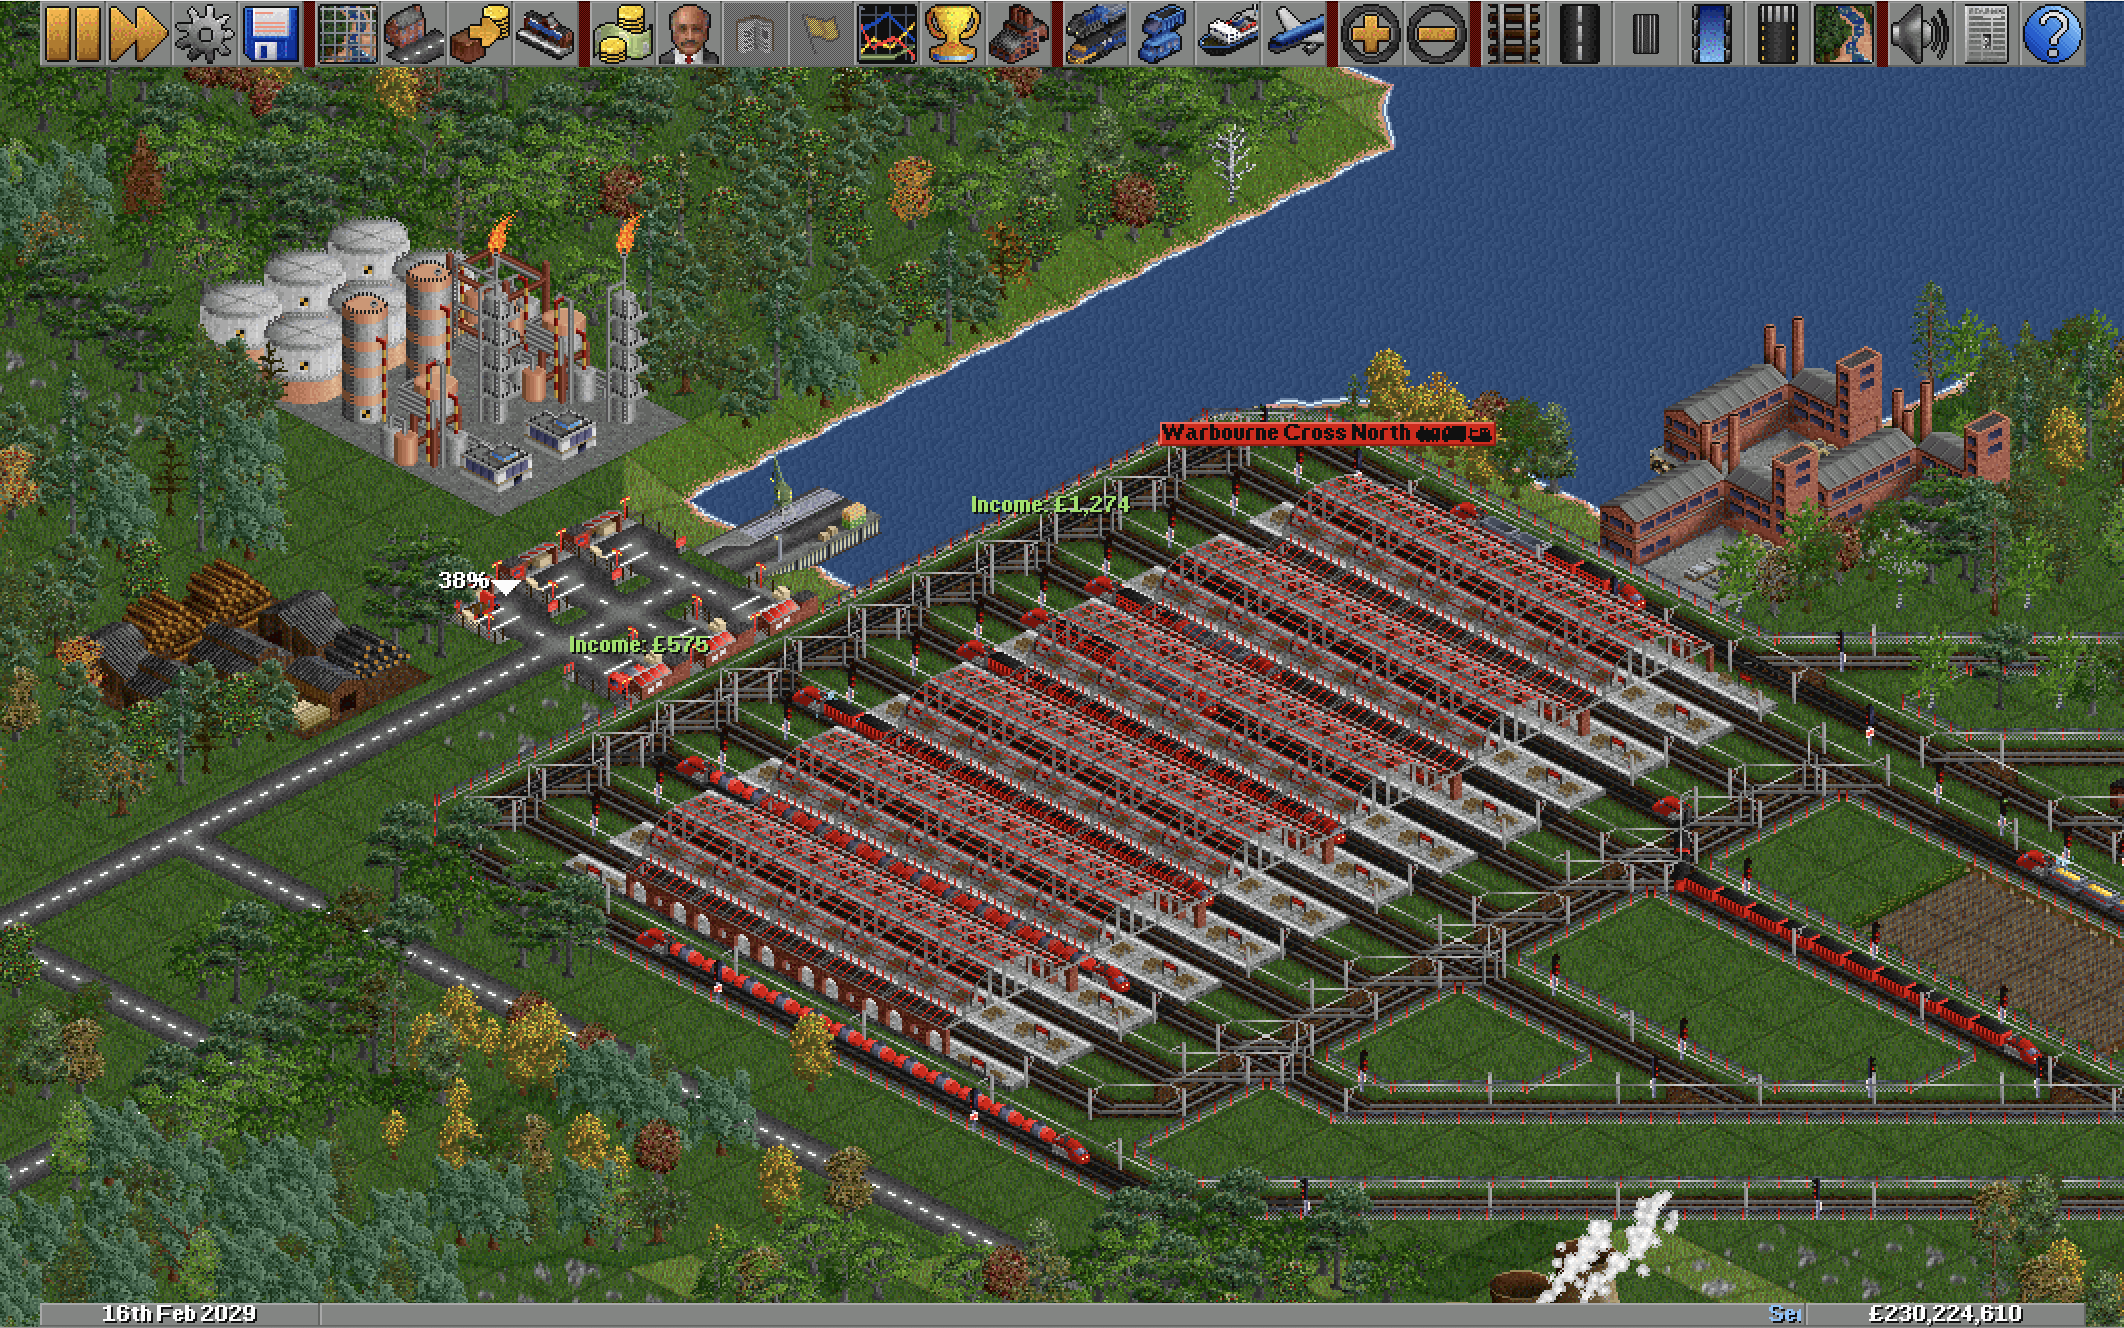
\includegraphics[width=\columnwidth]{assets/openttd_screenshot.png}
\caption{A small section of an OpenTTD version 13.4 game showing parts of a rail, road, and sea transportation network, as well as several industries. At the top is the control bar through which the player takes actions or see more details on the state of the game, such as finances.}
\label{figure:introduction-screenshot}
\end{figure}

OpenTTD was created as a game for recreation: it allows a single player to play in a non-competitive world building mode; multiple human players playing cooperatively or competitively; and so-called AI players, which via custom code that controls a company, provide opponents for humans to play against. However, it is remarkably flexible: it has been successfully used as a tool to research algorithms including artificial intelligence (AI), machine learning (ML), and anomaly detection algorithms where OpenTTD AI(s) play without human player involvement \cite{beuneker2019autonomous, bijlsma2014evolving, konijnendijk2015mcts, lakomy2020railroad, rios2009trains, wisniewski2011artificial, volna2017fuzzy}, scalability and mobile applications \cite{jiang2018mirroring}, and as a teaching aid for concurrency in computer programs \cite{HansenMuprhie2018, marmorstein2015teaching}\singlespacedfootnote{The work of Hansen \& Murphie \cite{HansenMuprhie2018} refers to an \emph{OpenTTD lab}, which is a set of scenarios and exercises for students to follow. It is not directly related to the OpenTTDLab presented here.} and for supply chain and logistics management \cite{doi:10.1080/10494820.2016.1242503}.

Simulation games have a long history of being used to inform government policies; see Raghothama \& Meije \cite{raghothama2013review} for a summary that focuses on logistics and simulation. In spite of this, no reference to using OpenTTD in this way has been found. A reason in Raghothama \& Meije \cite{raghothama2013review} is suggested: while some of the transportation aspects of the networks in OpenTTD are realistic, its economic model is not.

Of all these possible uses for OpenTTD, using OpenTTD as a tool for researching algorithms is the primary focus of the current work, and specifically the focus is the development of a reusable tool, OpenTTDLab, that augments the existing features of OpenTTD to improve its ability to be used in repeatable, reproducible, \& replicable research where OpenTTD AI(s) play without human player involvement. Given what is now the well-known replication crisis\singlespacedfootnote{The replication crisis is also known as the replicability crisis, the reproducibility crisis, and the credibility crisis.} \cite{ioannidis2005most, baker20161}, including in computer science \cite{dalle2012reproducibility, CollbergChristianProebsting2016}, if there are problems with how such research has been conducted using OpenTTD, as I will argue, then the potential usefulness of such a tool for future research is clear.

As a secondary and more speculative aim, it is hoped that the work here allows for OpenTTD to be investigated as a tool to simulate supply chain or transportation networks that could ultimately inform government policies. However, the nature of the correspondence between OpenTTD and what it is simulating must be determined, or in other words it must be \emph{validated} \cite{doi:10.1177/1046878198291003}.

\section[Repeatability, Reproducibility, \& Replicability: The 3Rs]{Repeatability, Reproducibility, \& Replicability:\texorpdfstring{\\}{ }The 3Rs}
\label{section:define-3rs}

The terms \emph{repeatability}, \emph{reproducibility}, and \emph{replicability}, the so-called \emph{3Rs}, unfortunately do not historically have universally agreed meanings \cite{plesser_reproducibility_2018}. Even the highly-cited 2016 Nature survey that reported that approximately 50\% of scientists believe there is a substantial reproducibility crisis \cite{baker20161}  uses the terms reproducible and replicable seemingly interchangeably. And both helpfully and confusingly, the Association for Computing Machinery (ACM) in 2020 swapped their definitions of reproducibility and replicability to align with the broader scientific community \cite{association_for_computing_machiner_new_2020}.

Choosing what I believe to be an authoritative source, I primarily use the post-swap ACM definitions from its \emph{Artifact Review and Badging Version 1.1} \cite{association_for_computing_machiner_artifact_2020}; these appear to broadly align with the definitions of \emph{The Turing Way} \cite{turingway2022}, a collaborative guide to reproducible data science spearheaded by the UK's national institute for data science and artificial intelligence, a similarly authoritative source. The ACM definition is given in terms of artifacts:

\begin{quote}
\begin{description}
\item[Artifact]

\ldots we mean a digital object that was either created by the authors to be used as part of the study or generated by the experiment itself. For example, artifacts can be software systems, scripts used to run experiments, input datasets, raw data collected in the experiment, or scripts used to analyze results.
\end{description}
\end{quote}
and the definitions of the 3Rs are:

\begin{quote}
\begin{description}
\item[Repeatability] (Same team, same experimental setup)

The measurement can be obtained with stated precision by the same team using the same measurement procedure, the same measuring system, under the same operating conditions, in the same location on multiple trials. For computational experiments, this means that a researcher can reliably repeat her own computation.
\item[Reproducibility] (Different team, same experimental setup)

The measurement can be obtained with stated precision by a different team using the same measurement procedure, the same measuring system, under the same operating conditions, in the same or a different location on multiple trials. For computational experiments, this means that an independent group can obtain the same result using the author’s own artifacts.

\item[Replicability] (Different team, different experimental setup)

The measurement can be obtained with stated precision by a different team, a different measuring system, in a different location on multiple trials. For computational experiments, this means that an independent group can obtain the same result using artifacts which they develop completely independently.
\end{description}
\end{quote}
%
These are not independent properties: reproducibility is unlikely to be achieved without repeatability \cite{hill2022reproducibility}, and replicability would be difficult to interpret in the absence of reproducibility \cite{nuijten2018verify}. While this highlights how the definitions are intertwined and therefore complex, it also means that a tool that eases repeatability eases reproducibility, a tool that eases reproducibility eases replication, and transitively a tool that eases repeatability indirectly eases replicability.

While ACM's definitions are clear in some respects, there is vagueness, especially in terms of what \emph{same result} means \cite{hill2022reproducibility}. In general, results can be said to be reproduced even if they are not exactly the same, i.e. not \emph{bitwise} identical. For example, in simulation studies if the original random seeds are not available but all other artifacts are, then results can still be said to be replicated if statistical results are the same \cite{luijken2024replicability}. Where appropriate I make a distinction between bitwise and non-bitwise reproducibility.

Note that the definition of artifact is limited to objects created by the authors; if research uses OpenTTD then it appears the research can be deemed replicated without OpenTTD itself having to be developed independently, simply because it was already available; to me this seems an unexpected loophole in the definitions. Similarly to how reproducibility can be bitwise or non-bitwise, if we extend the ACM definition of artifact to include other software used to generate the results, as I would argue we should, there appears to be degrees of replication that depend on how much of the original software used to run the simulation has been developed independently. It is beyond the scope of this project to deal with these issues in general, other than to ensure clarity as to what is or can be developed independently when discussing replication. In spite of the crisis being well known for approximately two decades, even as of May 2024 the replication of simulation studies is a ``novel endeavor'', 
and there are ``no set criteria to assess the alignment of replicated simulation results with the original results''~\cite{luijken2024replicability}; so I argue this a reasonable limitation to the scope of this project.

% \section{Barriers in achieving the 3Rs}

% The aim of OpenTTDLab is to help researchers achieve the 3Rs when using OpenTTD to research algorithms or, possibly, use OpenTTD to simulate transportation or logistic networks. As such it's important to note in general what barriers have been noted in similar research to achieving these.  Since the 3Rs are linked, de facto building on one another, it is unsurprising that barriers to achieving them are similarly linked, i.e. something that prevents one can prevent another. Here I summarise relateven barriers to achieving the 3Rs.

% Manual steps.

% Repeatability of computer simulations on the face of it should be the easiest to achieve, a researcher should \emph{reliably} repeat here own computation accor

% In terms or reproducing

% Through attempts to replicate statistical simulation studies, Luijken K et al. \cite{luijken2024replicability} construct a number of barriers to replication of studies. These 

% Why these barriers have not been overcome, especially in terms of the barriers to ensuring research is replicatable and repeatable, is usually due to a combination of their cost \cite{hernandez2023repeatability} and not sufficient reward. Reproducibility as a service has been.

% High cost is suggested, together . but the project here suggests an alternative: a tool to reduce that cost. Interestingly the tools used seems to be not studied. The closest things are preferring open source to prioprietry, and so-called reproducibility as a service. An Open Source framework for reproducible research appears to be novel.

\section{3Rs issues of existing OpenTTD research}

The aim of OpenTTDLab is to help studies that generate results by running OpenTTD without a human player and so only with AIs. From the first 100 results of a search for ``OpenTTD'' in Google Scholar in July 2024, seven existing studies have been found that do this: the work of Beuneker \cite{beuneker2019autonomous}, Bijlsma \cite{bijlsma2014evolving}, Konijnendijk \cite{konijnendijk2015mcts}, {Lakom{\`y} \cite{lakomy2020railroad}, Rios and Chaimowicz \cite{rios2009trains}, Wisniewski and Witt \cite{wisniewski2011artificial}, and Volna \cite{volna2017fuzzy}. Informally reviewing these in terms of how they have or have not seemingly achieved repeatability (the domain of the original researchers) or help achieve reproducibility or replicability (the domain of independent researchers), I found 7 problems. For brevity not all problems for all studies are listed.

\begin{itemize}

\begin{descitem}{Issue 1: Insufficient artifacts supplied to reproduce or analyse results}
One of the most complex and impressive studies is the work of Bijlsma \cite{bijlsma2014evolving} that used dynamic scripting to evolve the code of an OpenTTD AI using a genetic algorithm. In total there were at least 1250 experiments: 50 experiments each for 25 generations of the genetic algorithm, and after each of these, in-game metrics must have been extracted. There is nothing in OpenTTD that allows this to be done automatically, and it seems infeasible to have run this manually, especially because the AI code would be different each generation. It is mentioned in the text that a modified version of OpenTTD was used, but it does not describe how it was integrated with the genetic algorithm, and I was unable to find it to download.

Similarly the work of Konijnendijk \cite{konijnendijk2015mcts} suggests modifications of OpenTTD were made in order to extend its AI system with the algorithms presented in the work; I could not locate the code of these modifications, nor the code of the AIs that used them.

No study included the code used to analyse results or produce visualisations.
\end{descitem}

\begin{descitem}{Issue 2: Low or unknown number of repetitions}
While there is no one-size fits all number to how many repetitions an experiment must have, some of the studies I would argue have repetitions that are so few it makes me doubt the conclusions that are based on them. As examples, the two experiments of Rios and Chaimowicz \cite{rios2009trains} were run seven times each, the experiments of Wisniewski and Witt \cite{wisniewski2011artificial} were run just three times, and the work of Volna \cite{volna2017fuzzy} does not list the number of repetitions, nor even suggest there was more than one for each configuration.
\end{descitem}
\begin{descitem}{Issue 3: Non-comparable repetitions}
Rios and Chaimowicz \cite{rios2009trains} ran a total of 14 repetitions over 2 experiments, but not for the same amount of in-game time. This calls into question whether these were actually repetitions of the experiment.
\end{descitem}
\begin{descitem}{Issue 4: Manual repetitions of experiments and extraction of results}
No study explicitly stated that their experiments were run in an automated mechanism, and given the low number and non-comparable repetitions of some of the works, I suspect they were run manually, in that OpenTTD was configured and run through its graphical interface, which I suspect is tedious and error prone.

The study of {Lakom{\`y}} \cite{lakomy2020railroad} explicitly describes the manual mechanism uses to install and configure OpenTTD for its experiments. Having this description is excellent in terms of supporting reproduction of results, but the fact it is manual means it is high cost in terms of time to try to replicate its reported 50 repetitions.
\end{descitem}

\begin{descitem}{Issue 5: Insufficient detail on the version or configuration of OpenTTD}
The version of OpenTTD used to generate results is frequently omitted. For example, the work of Bijlsma \cite{bijlsma2014evolving} does not mention the version of OpenTTD that was then modified. Similarly the works of Volna \cite{volna2017fuzzy} and Beuneker \cite{beuneker2019autonomous} do not mention the version of, the presumably unmodified, OpenTTD used.

OpenTTD has a wide array of configuration options that can affect results, but it varies how well these are described. For example, the work of Wisniewski and Witt \cite{wisniewski2011artificial} describes the configuration exhaustively and in one place, but the work of Beuneker \cite{bijlsma2014evolving} only has limited detail, and what there is is spread throughout the work.
\end{descitem}
\begin{descitem}{Issue 6: No random seeds to bitwise reproduce results}
Possibly a special case of configuration, but it merits special attention since to gain statistical results typically experiments would be run for a fixed configuration over a range of random seeds. However, only one study reported the random seeds used: the work of Beuneker \cite{beuneker2019autonomous}. Not providing the random seeds impacts reproducibility, and specifically bitwise reproducibility: without the random seeds it is impossible to reproduce the results exactly.
\end{descitem}

\begin{descitem}{Issue 7: Insufficient or unclear detail of the algorithms to replicate results}
All of the studies included some high level detail of the algorithms implemented, but I found it difficult to judge if it each is sufficient to replicate results within the time constraints of the current work.

However, even if there is sufficient detail, in all cases bar one they are not presented in a way where replication appeared considered: the detail is spread throughout the work, and not presented as a clear algorithm or set of algorithms to be replicated. The exception is the work of {Lakom{\`y}} \cite{lakomy2020railroad}: it includes many algorithms each of them explained and discussed, although they are presented as snippets of code rather than pseudo-code. If these snippets of code were used, this would muddy the water between reproducing and replicating their results.
\end{descitem}

\end{itemize}
%
Determining replicability by reading the papers is certainly not as strong evidence as actually attempting to reproduce or replicate results. However, an independent researcher reading through a draft manuscript has been given as a recommendation to find issues before publication with the strongest of the 3Rs, replicability \cite{luijken2024replicability}; so I argue it is reasonable to extend the process to all of the 3Rs, and to base further actions, such as the creation of a framework to help avoid such issues, from such a review. While my review focused on OpenTTD, there are related wider problem in simulations in general: ``many published works based on simulation still fail to meet the minimum conditions to ensure reproducibility'' \cite{dalle2012reproducibility}.

\section{Reusability: The 4\texorpdfstring{\textsuperscript{th}}{th} R}

There is a 4\textsuperscript{th} concept given alongside ACM's definitions \cite{association_for_computing_machiner_new_2020}, not so much property of the results that the 3Rs focus on, but a property of the artifacts used to generate the results:

\begin{quote}
\begin{description}
\item[{[}Reusability{]}] 
The artifacts associated with the paper are of a quality that significantly exceeds minimal functionality. [\ldots] they are very carefully documented and well-structured to the extent that reuse and repurposing is facilitated. In particular, norms and standards of the research community for artifacts of this type are strictly adhered to. 
\end{description}
\end{quote}
Repeatability, reproducibility, and replicability are all in the realm of a single piece of research, but \emph{reusability} is concerned with the use of the artifacts to generate results of different-but-related research, possibly by other researchers. It is unfortunately often an afterthought in scientific software as it does not directly concern the current results the software is used to generate; but it has been argued that reusability helps reproducibility, and even increase the impact of the original work \cite{benureau2018re}. It is clear that a framework that helps with the 3Rs should itself be reusable and encourage reusable artifacts in work that uses it.

\section{Chapter outline}

The following chapters explain how OpenTTDLab helps experiments avoid issues with the 3Rs, especially the 7 issues listed, and in a reusable way. Chapter \ref{chapter:openttd-model-and-abilities} gives more background into OpenTTD: specifically what properties of OpenTTD make it suitable and interesting enough to research, what limitations it has, and at a high level how a framework could overcome at least some of these limitations. Chapter \ref{chapter:openttdlab-design-process-and-features} explains the design process I followed to create such a framework---the process itself provides an argument that it achieves its aims---and gives an overview of how its features help experiments be repeatable, reproducible, and albeit indirectly or through documentation, replicable. 

Chapters \ref{chapter:experiments-attempt-at-reproducing}--\ref{chapter:experiments-scaling} are the experimental chapters: they present results of experiments I ran using OpenTTDLab, and specifically they provide more evidence that there is a problem with existing OpenTTD research, and more direct evidence that OpenTTDLab can help with the 3Rs. Specifically, Chapter \ref{chapter:experiments-attempt-at-reproducing} explains how I attempted to reproduce existing published results, and while I did extract results, they did not fully match the ones originally published. Chapter \ref{chapter:experiments-attempt-at-reproducing} also shows that it is relatively straightforward to use OpenTTDLab to run experiments and extract results from them, and argues that these should be repeatable and reproducible. Chapter \ref{chapter:experiments-simple-parameterised-ai} gives the details of a simple OpenTTD AI that I constructed, and easily used with OpenTTDLab to extract results that appear to have real-world meanings, thus giving some evidence that by using OpenTTDLab, OpenTTD could be used to simulate the real world as part of the secondary aim of this work as mentioned earlier. \nolbreaks{Chapter \ref{chapter:experiments-simple-parameterised-ai}} also contains a clear description of the AI, and so should be replicable in the sense that another author should be able to construct a similar enough OpenTTD AI to replicate the results, possibly using OpenTTDLab. Chapter \ref{chapter:experiments-scaling} contains the results of a basic exploration of the performance of OpenTTDLab, showing how some of the features described in Chapter~\ref{chapter:openttdlab-design-process-and-features} help repeatability.

Chapter \ref{chapter:discussion} contains a discussion of what was found, summarises the limitations of the work, explores possible next steps, and compares OpenTTDLab to its closest equivalent. This dissertation finishes with a few concluding remarks in \nolbreaks{Chapter \ref{chapter:conclusion}}.

\chapter{OpenTTD: Its model and abilities}
\label{chapter:openttd-model-and-abilities}

A game of OpenTTD is made up of a rectangular world with one or more companies in it, typically working in competition against each other. A company is paid for transporting goods and passengers between certain combinations of industries and towns, and in order to do so it needs to invest in road, rail, sea or air infrastructure and vehicles.

When using OpenTTD for recreation there would be one or more human players that each control a company. However, as mentioned at the beginning of Chapter~\ref{chapter:introduction}, this is not a requirement: OpenTTD allows non-human players, so-called AI players, fully controlled by custom code. If there are no human players, OpenTTD then runs deterministically---using a seed value on startup that controls all pseudo-random behaviour of the game. These abilities are the core abilities that allows OpenTTD to be used in repeatable, reproducible, and hopefully, replicable simulations.

This chapter explores this model and these abilities in more detail, as well other related features that allow OpenTTD to be configured and ultimately used through the OpenTTDLab framework presented in the next chapter, to run simulations. This chapter also shows that the environment of OpenTTD is a rich one; while there are clearly some unrealistic aspects, it is at least a tempting target for running simulations that could be used to extract  insights about the real world.

Unless otherwise stated, the details here are from OpenTTD Wiki \cite{OpenTTDWiki}, the OpenTTD source code \cite{OpenTTDSource}, the OpenGFX source code \cite{OpenGFXSource}, the OpenTTD AI API documentation \cite{OpenTTDAIAPIDocs}, the OpenTTD GameScript API documentation \cite{OpenTTDGSAPIDocs}, or by playing OpenTTD itself. Details are correct as of OpenTTD 13.4.

\section{Field of play}

OpenTTD runs on a two-dimensional rectangular tiled grid representing an area of land and sea, with some limited three-dimensional aspects. The grid size is configurable on startup between $64 \times 64$ and $4096 \times 4096$ tiles. Each tile is square, albeit presented to the user in a dimetric view, as can be seen in Figure \ref{figure:introduction-screenshot}\footnote{A \emph{dimetric} view is sometimes inaccurately referred to as an \emph{isometric} view.}. Each tile does not necessarily have a single object on it, some objects can co-exist with each other depending on the object type. The positions of vehicles that carry cargo and passengers, which are the main mechanism for making money in the game, are even more granular: they move and appear to be able to take any position on their path between destinations.

There is some concept of height: each section of a grid can have one of a limited number of height levels in the game. This impacts the game in more than just a visual way: when going uphill road and rail vehicles usually slow down, and as discussed later in the current chapter, this can have an impact on money made. Rail and road tunnels can be built by the companies which can avoid this, but they have their downsides: for example they typically cost the company more to build, and can have their own speed restrictions.

\section{Startup}

There are two classes of startup: a pre-defined world or a pseudo-random world. In the pseudo-random case, which is the case of all experiments of Chapters \ref{chapter:experiments-attempt-at-reproducing}--\ref{chapter:experiments-scaling}, the world is deterministically generated from  the configuration of the game and an integer seed to the built-in random number generator, referred to as the \emph{random seed}. Specifically, the land, height, trees, coastlines, the sizes and positions of towns, and the positions and types of industries are all deterministically generated. This determinism means that OpenTTD can be used for bitwise repeatable and bitwise replicable experiments.

No transport infrastructure exists on startup other than roads within towns. It is the role of the players, including any AI players, to build these to connect towns and industries in order to earn income. On startup each company is provided a loan with which to begin building this infrastructure.

\section{Climates}

OpenTTD has four different \emph{climates}: \emph{temperate}, \emph{sub-arctic}, \emph{sub-tropical} and \emph{toyland}. A climate is fixed on game startup and effects a variety of properties of the game such as what transportation types are available, and what industries and supply chains are possible. For brevity all descriptions are limited to the default climate of temperate, as are the experiments of Chapters \ref{chapter:experiments-attempt-at-reproducing}--\ref{chapter:experiments-scaling}.

\section{Economic and transportation model}

The possible supply chains in the temperate climate of OpenTTD can be seen in Figure~\ref{figure:temperate-supply-chains}. In total there are 13 different types of industries that can produce or receive cargo: iron ore mines, coal mines, forests, farms, steel mills, oil wells, power stations, sawmills, factories, oil refineries, oil rigs, banks and towns; and 11 types of cargo: iron ore, coal, wood, livestock, grain, steel, oil, goods, valuables, mail and passengers. Towns and passengers are maybe not technically industries and cargo, but I include them because in terms of the economic model of OpenTTD they are.

\begin{figure}[ht]
\centering
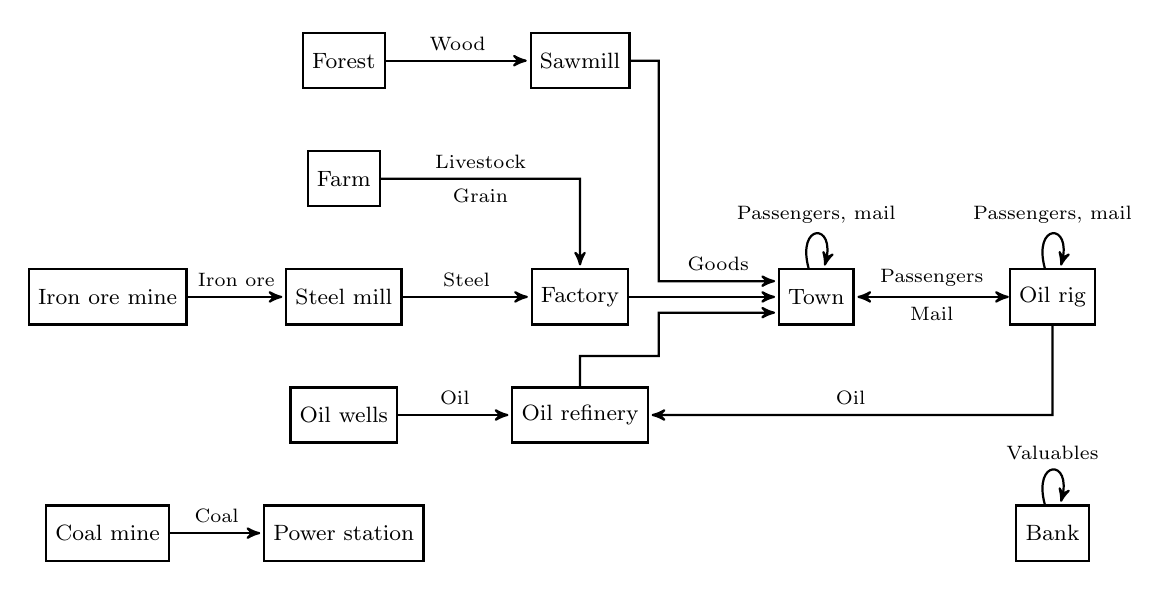
\begin{tikzpicture}[->,>=stealth',shorten >=1pt,auto,node distance=3cm,thick,main node/.style={rectangle,draw}]

    \node[main node, align=center,minimum size=0.7cm] (factory) {\footnotesize Factory};
    \node[main node, align=center,minimum size=0.7cm,on grid,right=3cm of factory] (town) {\footnotesize Town};
    \node[main node, align=center,minimum size=0.7cm,on grid,right=3cm of town] (oil-rig) {\footnotesize Oil rig};
    \node[main node, align=center,minimum size=0.7cm,on grid,left=3cm of factory] (steel-mill) {\footnotesize Steel mill};
    \node[main node, align=center,minimum size=0.7cm,on grid,left=3cm of steel-mill] (iron-ore-mine) {\footnotesize Iron ore mine};
    \node[main node, align=center,minimum size=0.7cm,on grid,below=1.5cm of steel-mill] (oil-wells) {\footnotesize Oil wells};
    \node[main node, align=center,minimum size=0.7cm,on grid,above=1.5cm of steel-mill] (farm) {\footnotesize Farm};
    \node[main node, align=center,minimum size=0.7cm,on grid,above=1.5cm of farm] (forest) {\footnotesize Forest};
    \node[main node, align=center,minimum size=0.7cm,on grid,below=3cm of oil-rig] (bank) {\footnotesize Bank};
    \node[main node, align=center,minimum size=0.7cm,on grid,below=1.5cm of oil-wells] (power-station) {\footnotesize Power station};
    \node[main node, align=center,minimum size=0.7cm,on grid,left=3cm of power-station] (coal-mine) {\footnotesize Coal mine};
    \node[main node, align=center,minimum size=0.7cm,on grid,right=3cm of forest] (sawmill) {\footnotesize Sawmill};
    \node[main node, align=center,minimum size=0.7cm,on grid,below=1.5cm of factory] (oil-refinery) {\footnotesize Oil refinery};

    \path[every node/.style={font=\scriptsize}]
        (forest) edge[] node[] {Wood} (sawmill)
        (bank) edge [loop above, distance=0.6cm] node[] {Valuables} (bank)
        (coal-mine) edge[] node[] {Coal} (power-station)
        (iron-ore-mine) edge[] node[] {Iron ore} (steel-mill)
        (oil-wells) edge[] node[] {Oil} (oil-refinery)
        (oil-rig) edge[loop above, distance=0.6cm] node[] {Passengers, mail} (oil-rig)
        (factory) edge[] node[] {} (town)
        (steel-mill) edge[] node[] {Steel} (factory)
        (town) edge[loop above, distance=0.6cm] node[] {Passengers, mail} (town);

    \path[draw,->] 
    (oil-rig.south)
    -- ($ (oil-rig.center) - (0,1.5) $)
    -- node[above] {\scriptsize Oil}
    (oil-refinery.east);

    \path[draw,<->] 
    (oil-rig.west)
    -- node[above] {\scriptsize Passengers} node[below] {\scriptsize Mail} 
    (town.east);

    \path[draw,->] 
    (farm.east)
    -- node[above] {\scriptsize Livestock} node[below] {\scriptsize Grain} ($ (farm.center) + (3,0) $)
    --
    (factory.north);

   \path[draw,->] 
    (oil-refinery.north)
    -- ($ (oil-refinery.center) + (0,0.75) $)
    -- ++(1,0)
    -- ++(0,0.55)
    -- ($ (town.west) - (0,0.2) $);

    \path[draw,->] 
    (sawmill.east)
    -- ($ (sawmill.center) + (1,0) $)
    -- ++(0,-2.8)
    -- node[above] {\scriptsize Goods} ($ (town.west) + (0,0.2) $);

\end{tikzpicture}
\caption{The possible supply chains of the temperate climate of OpenTTD 13.4, showing what types of cargo industries and towns accept and produce. Adapted from `Flow chart for Temperate Cargo' in the \emph{OpenTTD Wiki} \cite{TemperateFlowChart}.}
\label{figure:temperate-supply-chains}
\end{figure}
%
The companies in OpenTTD, controlled by either human or AI players, receive money for transporting the 11 cargo types between the 13 industry types. The amount of money is dependant on a number of
factors: the amount of cargo, the cargo type, and the time taken---a shorter time results in more money---and the distance between source and destination---longer distance results in more money. How much cargo each
industry or town outputs depends on a number of factors: for example, for an industry that receives cargo, its output depends on how much cargo it has recently received. This is similarly the case for towns: they grow in response to nearby activity and then ``produce'' more passengers ready to travel. The other factors are omitted for brevity.

The 11 cargo types can be transported by 4 classes of transportation: road, rail, sea and air; and each of these have further sub classes. With the exception of oil rigs, none of the industries have stations for transportation to pick up or drop off cargo, and so companies must build them at a cost. Stations can also only be built on flat or almost-flat land, which requires earth works which also costs. Companies must also build the road or rail networks to connect the stations. Road and rail networks cannot be built arbitrarily on sloping land: there are often earth works required to shape it which costs the company; this fact explains some of the results of Chapter \ref{chapter:experiments-attempt-at-reproducing}. With some exceptions, depots must also be built which are then used to build the vehicles that can transport the cargo. Once built, the company configures each vehicle with a route: a set of stations to travel between to pick up and drop off cargo; the minimum useful route is 2 stations long. Vehicles can break down and block other vehicles for a period of time; this depends on configuration, and the vehicle's type and age.

There are a number of obvious absurdities to the economic model. The number of good for example: there are 11 in OpenTTD, but the UK Tariff, the listing of all rules that govern imports into the UK, refers to over 25,000 different commodities \cite{uktariff}. Also, as long as an industry's type can accept a type of cargo according to the possible supply chains of Figure \ref{figure:temperate-supply-chains}, it will accept any amount of that cargo and will pay the company that transported it. It also doesn't matter which specific instance of an industry any particular piece of cargo is taken to. For example when a passenger arrives at a station, that particular passenger has no particular destination in mind---the company will receive money for taking them anywhere, but more money if they are taken further.

It is beyond the scope of this project to more rigorously analyse or validate the economic model of OpenTTD, and so to work out how much of any insights generated by OpenTTD simulations can be applied to the real world. As briefly mentioned in the previous chapter, it has been suggested that some of OpenTTD's network effects could be realistic, which presumably would involve the supply chains of Figure \ref{figure:temperate-supply-chains}. I hold out hope that OpenTTD could be used as a valid simulator for investigating such effects, and specifically by using OpenTTDLab.

\section{Agents, ticks, and threads}

OpenTTD is an agent-based system: buses, trains, planes, ships, industries and even buildings in towns run apparently independently and in accelerated real time. However, the real-time aspect is somewhat of an illusion. OpenTTD runs on the concept of \emph{ticks}, where there are 74 ticks per in-game day. During a tick game time progresses in a deterministic way: vehicles move a certain amount, pick up or drop off a certain amount of passengers or goods, industries produce a certain amount of goods, and a certain number of passengers wanting to travel are ``produced'' by towns and oil rigs.

This determinism makes OpenTTD particularly suitable for bitwise repeatable simulations. If for example, instead of ticks, threads were used for the various agents, since thread scheduling is in general non-deterministic, then bitwise repeatable experiments would not be possible. OpenTTD does use threads for secondary activities, such as showing progress bars or saving games, but with these exceptions the core of OpenTTD can be described as \emph{single-threaded}. This means that OpenTTD cannot speed up run time by leveraging the multiple CPU cores that are commonplace even on low-end computers: a possible issue if using it to run many repetitions experiments.

\section{OpenTTD AIs}

OpenTTD AIs are scripts written using the Squirrel language that can be plugged into OpenTTD at runtime in order to control a company. OpenTTD offers such AIs a rich API, with 545 functions to control the game or inquire into its state \cite{OpenTTDAIAPIDocs} where many of the functions act on specific tile(s) of the field of play. It works within the tick framework, in that every tick of the game only a certain amount of the AI script can progress. OpenTTD AIs can also be parameterised---accepting parameters set before the start of the game. For example, the AI created for the experiments of Chapter \ref{chapter:experiments-simple-parameterised-ai} accepts a single parameter that controls how many buses to create. For the avoidance of doubt, OpenTTD AIs can be extremely simplistic, without any of the advanced learning behaviour often associated with the term \emph{AI}.

The AI system is the core feature that allows OpenTTD to be used to research algorithms and hopefully simulate properties of the real world. The framework described in Chapter \ref{chapter:openttdlab-design-process-and-features} was designed to make it straightfoward to source, configure, and run such AIs, and all of the experiments of Chapters \ref{chapter:experiments-attempt-at-reproducing}--\ref{chapter:experiments-scaling} use them.

\section{Configurability}

OpenTTD has over 400 options set through a combination of its graphical interface or configuration file, and command line arguments; it is not useful to review them all here; see \cite{OpenTTDWiki} for the complete list and their defaults. However, there are several that are particularly relevant for repeatable, reproducible, or replicable experiments.

\begin{itemize}
\begin{descitem}{Properties of the pseudo-randomly generated world}
As suggested earlier, OpenTTD allows the configuration of the dimensions of the world, between $64 \times 64$ and $4096 \times 4096$ tiles. It also allows the specification of other related properties, such as if the generated world is flat or mountainous. Flat and mountainous worlds are compared in the experiments of Chapter \ref{chapter:experiments-attempt-at-reproducing}.
\end{descitem}
\begin{descitem}{Total number of ticks}
OpenTTD allows the specification of the number of ticks taken before it exits. This allows experiments to run for a fixed amount of in-game time, rather than the default of indefinitely. Each of the experiments of Chapters \ref{chapter:experiments-attempt-at-reproducing}--\ref{chapter:experiments-scaling} does this.
\end{descitem}
\begin{descitem}{Random seed}
As described earlier in this chapter, OpenTTD allows the specification of the random seed which controls how the world is generated at the start of play.

Keeping track of the random seeds allows experiments to be bitwise repeatable, and including the random seeds with published results should help them be bitwise reproducible. Each of Chapters \ref{chapter:experiments-attempt-at-reproducing}--\ref{chapter:experiments-scaling} includes the random seeds used.
\end{descitem}

\end{itemize}
%
OpenTTD also requires what's known as a \emph{base graphics set}. While this does not affect gameplay, it affects the visuals of the game. OpenGFX \cite{OpenGFXSource} is an open source base graphics set that is easily installable through the OpenTTD interface.

It should be noted that while OpenTTD has a wide range of options, there is nothing in OpenTTD to help run it over a specific range of configurations, for example over two different configurations of worlds, or over a range of random seeds.

\section{Extracting information}

OpenTTD 13.4 and earlier can be configured to automatically save the state of the game in intervals of in-game time in files of a custom binary format that are hierarchical in nature. These \emph{savegames} [sic] are designed to resume games after interruption, but they are also rich sources of information for analysis, containing for example the complete transportation network each company has constructed, how much each company is worth, or how much money it has. OpenTTD 14.0 no longer has deterministic saving, but there is a way to restore this ready for OpenTTD 15.0.\footnote{OpenTTD 14.0 changed how games were saved from intervals of in-game time to intervals of wall-clock time, which makes the savegames non-deterministic, and so makes it virtually impossible to use them to extract information from OpenTTD for bitwise repeatable experiments. However, as part of this project I successfully submitted a change to OpenTTD that allows the scheduling of so-called \emph{console scripts} that can be used to restore the behaviour of OpenTTD 13.4 \cite{OpenTTDScheduleScript}. This change is scheduled for release in OpenTTD 15.0.}

It is notable that no version of OpenTTD has a built-in ability to extract detailed information from these savegames in a form suitable for analysis, or indeed aggregate such information over multiple savegames in order to see changes over in-game time. Also in spite of their richness and deterministic nature, so far there is no evidence of existing research using savegames to extract information from OpenTTD; I suspect instead information was usually extracted manually through its graphical interface.

\section{Conclusion}

OpenTTD presents an extremely rich landscape for investigation; and because of its tick model, and the fact it accepts a random seed, this landscape is deterministic and so especially suitable for repeatable research. While its economic model is simplified or even absurd in parts, depending on the map size, there are hundreds of millions of possible actions an OpenTTD AI can take on any given tick of the game, and the existing research has only begun to explore this space.

If viewing OpenTTD not as a game for which it was designed, but as a tool for running repeatable, reproducible, and hopefully replicable research, there are three core features that are not present in OpenTTD. Firstly, there is no way to configure OpenTTD so it runs over a range of available configurations, for example over a range of random seeds. Secondly, while it saves information to its savegame files, there is no way to extract and combine this information into a form ready for analysis. And thirdly, while OpenTTD is largely single-threaded, which contributes to its determinism and bitwise repeatability and reproducibiliy, it means it has no way to leverage multiple CPU cores. These are the core features that OpenTTDLab, as described in the next chapter, effectively add to OpenTTD.

\chapter{OpenTTDLab: Its design and features}
\label{chapter:openttdlab-design-process-and-features}

\begin{figure}[H]
\centering
\includesvg{assets/openttdlab-logo.svg}
\caption{The OpenTTDLab logo. I created this based on the existing OpenTTD logo (licensed under GPLv2) \cite{OpenTTDLogo}, and it is displayed alongside the code of OpenTTDLab in its public documentation, as can be seen in Appendix \ref{chapter:openttdlab-documentation}.}
\label{fig:openttlab-logo}
\end{figure}

As discussed in Chapter~\ref{chapter:introduction}, repeatability is the domain of the original researchers, while reproducibility and replicability are the domain of other researchers armed with the results of the original research. Given the different aims and audiences, it's not immediate that a single tool can help with all of these. However, the Python framework I created, OpenTTDLab, attempts to do this by adding the missing features described at the end of the previous chapter to help address the 7 issues detailed in Chapter~\ref{chapter:introduction}. The current chapter details the design process I followed to create OpenTTDLab, and some of the resulting internal behaviours and user-facing features of the framework.

\section{Design and creation process}

I used a lightweight and highly-agile process to design and create OpenTTDLab; the high level features of this process are shown Figure \ref{fig:solo-agile}. After I identified the problems to address, as discussed in Chapter~\ref{chapter:introduction}, I conducted many cycles of writing documentation for code, writing code, and using the code, either to conduct the experiments of Chapters~\ref{chapter:experiments-attempt-at-reproducing}--\ref{chapter:experiments-scaling} or in tests; and each of these with tight cycles of evaluating the outputs of these activities and informally judging if the code does---or would if it existed---help produce research that is repeatable, replicable, and reproducible. Each of these activities would inform each other, again in tight cycles.
%
\begin{figure}[ht]
\centering
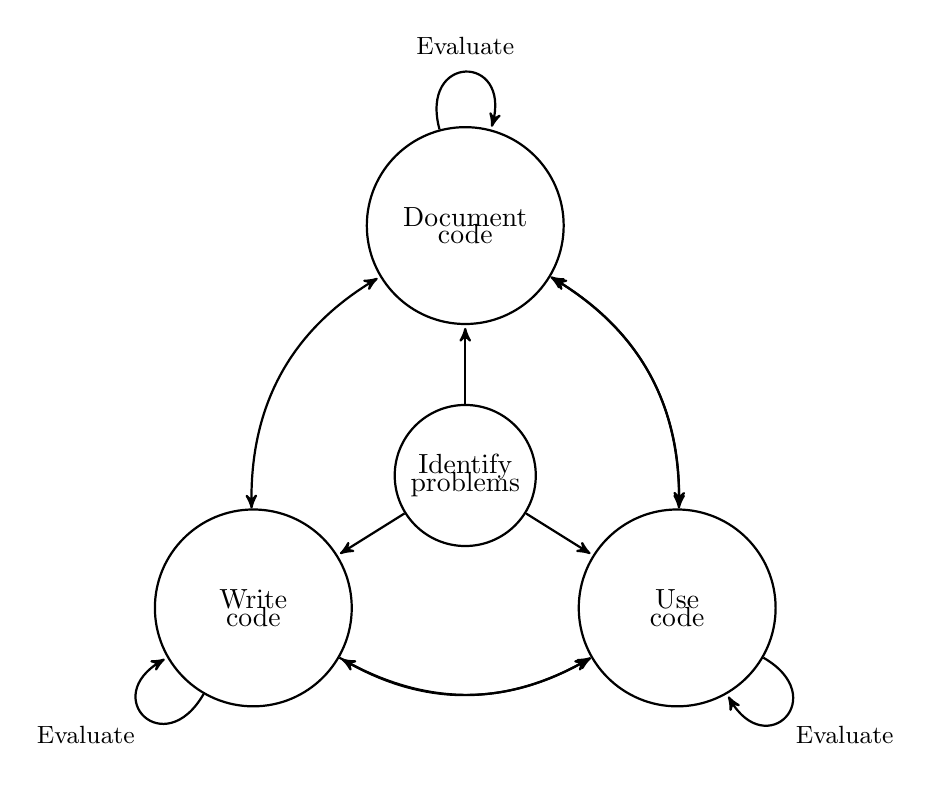
\begin{tikzpicture}[->,>=stealth',shorten >=1pt,auto,node distance=3cm,
                    thick,main node/.style={circle,draw}]

    % https://tex.stackexchange.com/a/102266
    \tikzset{
        position/.style args={#1:#2 from #3}{
            at=(#3.#1), anchor=#1+180, shift=(#1:#2)
        }
    }

    \node[main node, align=center] (reqs) {Identify\\[-2mm]problems};
    \node[main node, align=center,minimum size=2.5cm] (code) [position=90:1cm from reqs] {Document\\[-2mm]code};
    \node[main node, align=center,minimum size=2.5cm] (docs) [position=-148:1cm from reqs] {Write\\[-2mm]code};
    \node[main node, align=center,minimum size=2.5cm] (expe) [position=-32:1cm from reqs] {Use\\[-2mm]code};

    \path[every node/.style={font=\small}]
        (reqs) edge [] node[] {} (code)
               edge [] node[] {} (expe)
               edge [] node[] {} (docs)
        (docs) edge [in=-150,out=-120,distance=1cm,loop] node[] {Evaluate} (docs)
               edge [bend left,arrows=<->] node[] {} (code)
               edge [bend right] node[left] {} (expe)
        (code) edge [distance=1cm,loop above] node[yshift=0.1cm] {Evaluate} (code)
               edge [bend left,arrows=<->] node[] {} (expe)
        (expe) edge [in=-60,out=-30,distance=1cm,loop] node {Evaluate} (expe)
               edge [bend left,arrows=<->] node[] {} (docs)
               edge [bend right,arrows=<->] node[] {} (code);
\end{tikzpicture}
\caption{The process I followed designing and creating OpenTTDLab. After identifying the problems that I'm trying to address, I conducted cycles of documenting code (that may not have existed), writing the code, and using the code, all coupled with tight cycles of evaluating how it solved, or would solve, the problem of running experiments using OpenTTD that were repeatable, replicable and reproducible.}
\label{fig:solo-agile}
\end{figure}
%
I describe the process as \emph{lightweight} because were no \emph{events} that are common to \emph{Scrum}-like processes \cite{SCRUM}\footnote{From my own experience Scrum events are often known as \emph{ceremonies}}, and with one exception, no phases planned in advance as is often prescribed, for example for UK government services \cite{GOVUKAgile}. And I describe the process as \emph{highly-agile} because in some cases iterations would take a low number of seconds, especially when writing documentation.

There was in fact the one exception to not having phases planned in advance: I did plan to create an initial version of light usage documentation very early in the project. Taking inspiration from Tom Preston Warner's Readme driven development \cite{ReadmeDrivenDevelopment} and Amazon's Working Backwards method \cite{bryar2021working}, throughout the project, but especially at the beginning, I would write documentation for code without the code actually existing. This allowed me to imagine it being used, evaluate how well it would solve the problems I'm trying to solve, and change its design accordingly by quickly changing its documentation. Of course documentation for code that does not exist has very little value, so I moved quickly to writing and using code, mostly informed by the ``Working software is the primary measure of progress'' and ``Deliver working software frequently'' principles of the Agile Manifesto \cite{beck2001manifesto}, which I judge to be the most useful principles of the Agile Manifesto, especially when working alone, albeit with advice from others. The other principles are less applicable---they focus on communication between different people involved in project.

I did not attempt to keep a precise record of the cycles. However, as a guide the GitHub repository that stores the history of code changes can be used \cite{OpenTTDLab}. I created 72 releases, which I labelled v0.0.1 through v0.0.72, 215 pull requests (PRs), and over 250 non-merge commits in the repository, and each of these I evaluated against the problems and desired properties of Chapter~\ref{chapter:introduction}. I then carried on with more of the same activity, or another activity of Figure \ref{fig:solo-agile}. A summary of the releases can be seen in Appendix~\ref{chapter:openttdlab-releases}.

The first version, v0.0.1, was the result of a fork from Patric Stout's \emph{OpenTTD-savegame-reader} \cite{Stout2024}, an existing Python project that extracts data from OpenTTD savegame files---as described in Chapter~\ref{chapter:openttd-model-and-abilities} these are files that save the state of play in OpenTTD that allows players to exit but resume at the same point later. This project could be be used to extract data from OpenTTD, and seemed a reasonably place to start. However, as mentioned in the same chapter, even with this code there was still no way to easily run OpenTTD over a range of configurations, or extract information from the savegame files in bulk, and no way to leverage multiple CPU cores.

Then, but still from very early in the process, v0.0.3, I created and maintained a small suite of tests for OpenTTDLab, asserting on its high level behaviour. However, the tests were not just for asserting on the behaviour of the code, they were also a special case of ``Use code'' in the design process of Figure~\ref{fig:solo-agile}; they allowed me to extremely quickly gauge the suitability of the design of OpenTTDLab, because to write these tests I used OpenTTDLab in a way very similar to the ways researchers would use it. I also configured these test to run automatically on every change: a ``very helpful'' property for software used in reproducible research according to \emph{The Turing Way}~\cite{turingway2022}. The tests essentially use OpenTTDLab to run experiments and assert on their results; they must be identical to previous runs of the experiments to pass, and so themselves give evidence that OpenTTDLab can be used to run bitwise repeatable experiments.

This leads to the main downside of this process: while the process allowed a high number of cycles of evaluations, all evaluation was from myself, from either running the code or, even worse, just imagining running the code. Being the creator I knew it extremely well and so was ill-placed to evaluate what amounts to its ease of use for people that don't know it as well: I'm essentially \emph{marking my own homework}, and in some cases before it was even written. This is true when writing any code, but in this case this is especially true as there are different groups of people in the target audience: original researchers, reproducers, and replicators. User research was not included in the process in order to limit the scope of the project and to allow as many iterations as possible within the available time. However, while making OpenTTDLab I conducted the three different experiments of Chapters \ref{chapter:experiments-attempt-at-reproducing}--\ref{chapter:experiments-scaling} in which I played multiple roles: I conducted original research and used OpenTTDLab to attempt to reproduce existing research, and so partially mitigated this downside.

\section{Python and portability}

% Through the design and creation process, particularly after evaluation, I made a number of high level architectural decisions: the use of Python, behaving identically where possible on different platforms, automatically downloading OpenTTD and OpenGFX, supporting both AIs in the local filesystem, and automatically downloading AIs, caching, and the use of parallelisation.

I chose Python as the main language for both the internals of OpenTTDLab and its user-facing interface. I knew Python well, as mentioned earlier in this chapter a savegame parser for OpenTTD was available in Python \cite{Stout2024}, programs written in Python are mostly platform independent, and anecdotally it's a popular language in data science and data analysis---data analysis and visualisation can be performed in Python through libraries such as Pandas \cite{mckinney-proc-scipy-2010,reback2020pandas,} and Plotly \cite{plotly}. To make sure OpenTTDLab did not depend on behaviour unique to a single Python version or a single platform, which would impede reproducibility of experiments especially \cite{turingway2022}, I made OpenTTDLab \emph{portable}---hiding platform-specific details, and making sure that the tests mentioned in the previous section run and pass on multiple version of Python, but also on Linux, Windows and macOS. While OpenTTD itself is classed as portable, downloading, uncompressing, configuring, and starting OpenTTD are slightly different on each platform, so running tests on each is particularly valuable when considering reproducibility.

\section{Feature 1: Running over a range of configurations}

OpenTTDLab can run a specific version of OpenTTD and OpenGFX over a range of configurations: a range of random seeds and range of other configurations, and a range of OpenTTD AIs and their parameters with the numbers of runs made clear. During these experiments a progress bar is shown to the user to show the approximate proportion of experiments complete at any given moment. This is all through a single Python statement, with no steps ahead of time needed other than the installation of Python and OpenTTDLab. This requires that under the hood OpenTTDLab downloads and caches OpenTTD, OpenGFX, and OpenTTD AIs and libraries they depend on published on GitHub or OpenTTD's TCP-based BaNaNaS [sic] content publishing service \cite{OpenTTDBaNaNaS}, or on the local file system. An example use of OpenTTDLab can be seen in Listing \ref{listing:openttdlab}.

\begin{lstlisting}[label=listing:openttdlab,language=Python, caption={Example usage of OpenTTDLab that runs the trAIns AI automatically downloaded from BaNaNaS for a single year of in-game time for random seeds 0 to 9.}]
from openttdlab import run_experiments, bananas_ai

results = run_experiments(
    openttd_version='13.4',
    opengfx_version='7.1',
    experiments=(
       {
         'seed': seed,
         'ais': (
             bananas_ai('54524149', trAIns', ai_params=()),
         ),
         'days': 365 * 4 + 1,
       }
       for seed in range(0, 10)
    ),
)
\end{lstlisting}
%
Keeping to a single Python statement with no steps required ahead of time I found extremely convenient for repeatability, and I argue is important for reproducibility because it means only a small amount of Python code needs to be shared as an artifact, with no additional information required other than the version of Python and OpenTTDLab; although as discussed the version of Python should not affect the results.

\section{Feature 2: Output as lists and dictionaries}

As noted one of the missing features of OpenTTD, if viewing it as a simulator rather than a game, was the fact that data output was in a series of binary savegame files of a custom format: not in a format immediately suitable for analysis. I decided to convert all the savegame files from all the runs of OpenTTD into a single partially self-documenting data structure: a Python list of dictionaries.

This means that OpenTTDLab is agnostic to the specific way of how a user would prefer to analyse output; or in the language of Chapter~\ref{chapter:introduction} it is reusable in this respect. But as can be seen in Listing~\ref{listing:openttdlab-analyse}, only a single statement is required to convert a subset of the output into a Pandas \emph{data frame}, a common first step when using Pandas to analyse data.

\begin{lstlisting}[label=listing:openttdlab-analyse,language=Python, caption={Example usage of the results of OpenTTDLab, such as those generated in \ref{listing:openttdlab}, converting them to a Pandas data frame.}]
import pandas as pd

df = pd.DataFrame(
    {
        'seed': row['experiment']['seed'],
        'date': row['date'],
        'money': row['chunks']['PLYR']['0']['money'],
    }
    for row in results
)
\end{lstlisting}
%
An alternative would be to output Pandas data frame(s) directly from OpenTTDLab. However, the main downside of this approach is that I would have to design a structure for the data frame(s), but since OpenTTD savegame data is hierarchical there is no unique or one-size-fits-all approach to convert such data into such data frames. Any approach would have pros and cons, and to investigate these I decided was out of scope of the current work. For similar reasons I rejected saving the results to A non-ephemeral file such as SQLite: a tempting target since SQLite is a preferred format for datasets according to the US Library of Congress \cite{sqlitelog}. How to save data non-ephemerally is left to client code; for example a simple CSV format can be chosen to save a subset of the output, which is the approach I chose to persist the results of Chapters \ref{chapter:experiments-attempt-at-reproducing}--\ref{chapter:experiments-scaling}.

Early on in the design process, in v0.0.2, I considered structuring both the API and the output to have a required \emph{verification} step to make it easier to confirm that both configuration and results were bitwise identical to previous experiments. While this might have been particularly useful for determining if results have been bitwise reproduced, it made generating the results of Chapters \ref{chapter:experiments-attempt-at-reproducing}--\ref{chapter:experiments-simple-parameterised-ai} particularly awkward. Or in other words it seemed like this would negatively affect the reusability of OpenTTDLab, and for this reason I abandoned this approach.


\section{Feature 3: Leveraging multiple CPU cores}

OpenTTDLab leverages multiple CPU cores by implementing simple task-based parallelism: it starts a process per experiment, which runs OpenTTD, extracts data from its savegames, serialises it, and returns it to the controlling process. By default the number of processes is the number of CPU cores on the system. To further reduce time, a mechanism to reduce the amount of data returned by each process is available. These features I added to OpenTTDLab to help repeatability: specifically to run more repetitions of experiments in a given amount of time. A contributing reason was my own frustration while waiting for experiments to complete in the original single core version; I suspected that others using OpenTTDLab would feel similar frustration, and repeat experiments a fewer number of times.

\section{Documentation}

As discussed, writing documentation was part of the design process. However, since documentation is especially important for reusable software used for reproducible research \cite{turingway2022}, this documentation I repeatedly extended and published alongside OpenTTDLab, as it can be seen in Appendix \ref{chapter:openttdlab-documentation}. In addition to usage instructions, examples, and API documentation, it includes recommendations relating to the repeatability, reproducibilty and replicability of work that uses OpenTTDLab; replicability is addressed by encouraging authors to include details of the algorithms used in OpenTTD AIs created as part of the work.

As part of the documentation process I made a logo for OpenTTDLab based on the OpenTTD logo, as can be seen in Figure~\ref{fig:openttlab-logo}. I did not have a rigorous justification for this, but I suspected that creating an identity for OpenTTDLab, especially one that was related to the identity of OpenTTD itself, would encourage the reuse of OpenTTDLab, and even encourage contributions to it.

% \section{Algorithm}

% \begin{algorithm}
% \caption{The core algorithm of OpenTTDLab}\label{alg:openttd}
% \KwData{The list of experiments to run, where each is defined by the seed, number of days, list of AIs and parameters to pass to the AIs. Versions of OpenTTD and OpenGFX}
% \KwResult{The parsed save games from every month of game time for every experiment} 
%  fetch everything that needs to be fetched (not stuff that is already in cache...)\;
%  setup threaded pool for workers\;
%  \ForEach(in parallel up to {max\_workers}){experiment in experiments}{
%   run experiment by running OpenTTD\;
%   parsing all the save games\;
%  }
% \end{algorithm}

\section{OpenTTDLab and the 3Rs issues}

The three features of OpenTTDLab address 6 of the 7 issues in existing OpenTTD research described in Chapter~\ref{chapter:introduction}. Because of the low amount of Python code needed to run experiments and analyse results, it should be straightforward to include these artifacts in published work, or at least make the code available separately and link to it (Issue 1). OpenTTDLab leverages multiple cores and so supports running more repetitions in a given amount of time, and sharing the Python artifacts shares how many repetitions were run (Issue 2). As can be seen from Listing \ref{listing:openttdlab}, it is straightforward to run multiple experiments  over the exact same amount of in-game time (Issue 3). There are no manual steps involved to download, configure, or run OpenTTD or extract data (Issue 4). The versions of OpenTTD, OpenGFX, and details of configuration are included in the artifacts (Issue 5), which also includes the random seeds used (Issue 6).

The issue of replicating results (Issue 7) is not directly addressed by features of OpenTTDLab. However, this is still addressed in two ways: as mentioned in the previous section, its documentation encourages authors that use OpenTTDLab to include explicit details of the algorithms created; and by the transitive nature of the 3Rs described in Chapter~\ref{chapter:introduction}, helping repeatability and reproducibility indirectly aids replicability.

\section{Conclusion}

OpenTTDLab offers three features through a single Python statement: it allows a researcher to easily run OpenTTD over a range of configurations, including running ranges of AIs; it returns results from these experiments in a way that's suitable for analysis; and it leverages multiple CPU cores which allows more experiments to be run in a given amount of time. These are all useful for repeating experiments; if artifacts are shared, then reproducing experiments; and if the algorithm of OpenTTD AIs created are shared as encouraged by the OpenTTDLab documentation, also replicating experiments.

In the following chapters I give more direct evidence of OpenTTDLab's usefulness in repeating and replicating by using OpenTTDLab in experiments. In Chapter~\ref{chapter:experiments-attempt-at-reproducing}, I play the role of replicator, using OpenTTDLab to attempt to replicate existing research. In Chapter~\ref{chapter:experiments-simple-parameterised-ai}, I play the role of original researcher, creating a simple OpenTTD AI; also suggesting that OpenTTD is a compelling landscape for simulation and worthy of further research. In Chapter~\ref{chapter:experiments-scaling}, I provide evidence that the parallelism features added actually work, and argue that this helps repeatability.

% \chapter{Example results}

% To get validate of OpenTTDLab's usefulness in terms of repeatable, reproducible and replicable experiments, I used OpenTTD in 3 different situations. Firstly, to attempt to reproduce existing results from authors of an existing OpenTTD AI, and even in one respect go further in terms of showing what results are possible to extract and analyse. Secondly, to explore how a single parameter can change how a new simple AI performs, and shows that OpenTTDLab can be used to explore risk-benefit trade offs in basic supply chains. And finally to show how OpenTTDLab can be used to programmatically optimize this parameter using a basic algorithm.

\chapter{Experiments 1: Reproducing results}
\label{chapter:experiments-attempt-at-reproducing}

To attempt to validate OpenTTDLab as a useful framework, I used it to attempt to reproduce some of the results of Rios and Chaimowicz \cite{rios2009trains}: a set of experiments running two AIs, trAIns [sic] being presented in the aforementioned work, and the pre-existing AdmiralAI; and I compared their company values. I generated results, and while trAIns does appear to perform better than AdmiralAI as the original results suggest, the performance of trAIns does not match that of the original work.

\section{Experimental setup}

The setup was a best-effort attempt to match what was described as the setup of the experiments in the original work: the starting year was set to 1960, the map was configured to be $512 \times 512$ with a very low amount of seas, industry density and number of towns set to normal, the economy set to be able to fluctuate, subsidy multiplier of $\times 2$, disasters enabled, tolerance of town councils to changes set as tolerant, both vehicle running costs and construction costs set to medium, vehicle breakdowns disabled, trains set to only be able to turn around at the end of the line as opposed to also at stations, the maximum initial loan was set to £300,000, and the initial interest rate set to 3\%.

Note that these settings are not all explicitly mentioned in the original paper: it describes running OpenTTD revision 16724 using the \emph{medium} difficulty level with some overrides. However, due to savegame format differences OpenTTDLab does not work under this version, and the recent versions of OpenTTD that do work under OpenTTDLab no longer have the concept of difficulty level. However, the historical meaning of the medium difficulty level is documented \cite{OpenTTDDifficultyLevels}, and so the explicit list of aforementioned settings recreated, and run under OpenTTD 13.4 and OpenGFX 7.1 that OpenTTDLab does work under. There was one exception to basing off the medium difficulty level: the medium difficulty level was documented to have a maximum initial loan of £150,000, but using this level in pilot experiments resulted in extremely poor performance of AdmiralAI---it appeared to be virtually unable to function.

None of the versions of the AIs or their dependencies were specified in the original paper. In the current experiments, the version of trAIns is 2.1,  the version of AdmiralAI is 25, and the version of AdmiralAI's single dependency, Queue.FibonacciHeap, is 2. All the AIs and their dependencies were retrieved from BaNaNaS.

The results presented here are for exactly 15 years of in-game time, while in the original work the time varied from 15 years and 2 days to 15 years and 11 months. In both the original paper and here, there were two sets of experiments performed: one on the \emph{flat} terrain type, and one on the \emph{mountainous} terrain type. Here each set contains 64 repetitions, and in the original paper each set contains 7 repetitions. Here random seeds 0 to 63 were used for each set of experiments, but in the original paper the random seeds are unknown.

The experiments here were run on mac OS 14.5 running on a 2020 M1 and Python 3.11.0 and OpenTTDLab 0.0.72. The OS and CPU of the original experiments are unknown. The experiments here were run with OpenTTDLab's default number of workers---the number of cores on the machine---which in this case was 8.

The Python code used to run the experiments is in Appendix \ref{chapter:trains-vs-admiral-run-experiments}, and the code to subsequently analyse the results in Appendix \ref{chapter:trains-vs-admiral-analyse-results}.

\section{Results}

The results of the experiments can be seen in Figure \ref{figure:trains-ai-vs-admiral-ai-final-distributions}, showing the final distributions of company value for the two sets of experiments for each of trAIns and AdmiralAI, comparing the results using OpenTTDLab to the results of the original paper; and in Figure \ref{figure:trains-ai-vs-admiral-ai-over-time}, showing how the distribution of company value changes over time for the two sets of experiments and two AIs, but not comparing them with the original paper because it did not include sufficient data.

From \ref{figure:trains-ai-vs-admiral-ai-final-distributions} it is clear that while trAIns performed better than AdmiralAI in both OpenTTDLab and original experiments, the difference between the two AIs in the current experiments is slight, as opposed to the original paper when the difference was remarkable. While AdmiralAI's performance is similar or slightly worse than what was originally reported, especially in the mountainous configuration, trAIns can be characterised as approximately an order of magnitude worse. It can also be seen that in the current experiments there are more cases that can be classed as catastrophic---in the sense that the company value remains approximately zero---across both trAIns and AdmiralAI.

The results over time of Figure \ref{figure:trains-ai-vs-admiral-ai-over-time} show that for both trAIns and AdmiralAI the distribution of company value becomes increasingly wider with time. They also show that while the median value for trAIns is slightly higher than for AdmiralAI, the distribution of company value for trAIns is much wider than that for AdmiralAI, especially on flat terrain.

From Figures \ref{figure:trains-ai-vs-admiral-ai-final-distributions} \& \ref{figure:trains-ai-vs-admiral-ai-over-time} it can be seen that in both the original and current experiments, both AIs appeared to perform better on flat terrain than on mountainous.

\begin{figure}[p]
\centering
\begin{gnuplot}[terminal=cairolatex,terminaloptions={size 5.5,3}]
file = "notebooks/01_trains_ai_vs_admiral_ai_results_02_combined_final.csv"
set datafile separator ","
set grid ytics
set format y "\\footnotesize %.0s%c"
set style data boxplot 
set style boxplot outliers pointtype 1 medianlinewidth 2
set style boxplot fraction 1.00
set ylabel '\footnotesize Company value $\textrm{\pounds}$'
set key right top

mylabel(name) = sprintf("%s", name)
set style fill pattern 2 border lt -1

set multiplot layout 1,2
set yrange [-2500000:50000000]
set ytic 5000000

set xlabel ""
set lmargin at screen 0.11; set rmargin at screen 0.53
set xtics ("\\footnotesize trAIns" 1.5, "\\footnotesize AdmiralAI" 3.5)
set label 1 '\footnotesize Flat' at graph 0.03,1.05
plot file \ 
   using (1):(strcol(6) eq "Original paper" && strcol(4) eq "Flat" && strcol(2) eq "trAIns AI" ? $3 : NaN):(0.5) lc rgb '#aaaaaa' fs pattern 2 notitle, \
   '' using (2):(strcol(6) eq "OpenTTDLab" && strcol(4) eq "Flat" && strcol(2) eq "trAIns AI" ? $3 : NaN):(0.5) lc 2 fs pattern 0 notitle, \
   '' using (3):(strcol(6) eq "Original paper" && strcol(4) eq "Flat" && strcol(2) eq "Admiral AI" ? $3 : NaN):(0.5) lc rgb '#aaaaaa' fs pattern 2 notitle, \
   '' using (4):(strcol(6) eq "OpenTTDLab" && strcol(4) eq "Flat" && strcol(2) eq "Admiral AI" ? $3 : NaN):(0.5) lc 2 fs pattern 0 notitle

set xlabel ""
unset ylabel
set format y ''
set lmargin at screen 0.53; set rmargin at screen 0.95
set label 1 '\footnotesize Mountainous' at graph 0.03,1.05
plot file \ 
   using (1):(strcol(6) eq "Original paper" && strcol(4) eq "Mountainous" && strcol(2) eq "trAIns AI" ? $3 : NaN):(0.5) pointsize 0.5 lc rgb '#aaaaaa' notitle, \
   '' using (2):(strcol(6) eq "OpenTTDLab" && strcol(4) eq "Mountainous" && strcol(2) eq "trAIns AI" ? $3 : NaN):(0.5) pointsize 0.5 lc 2 fs pattern 0 notitle, \
   '' using (3):(strcol(6) eq "Original paper" && strcol(4) eq "Mountainous" && strcol(2) eq "Admiral AI" ? $3 : NaN):(0.5) pointsize 0.5 lc rgb '#aaaaaa' fs pattern 2 notitle, \
   '' using (4):(strcol(6) eq "OpenTTDLab" && strcol(4) eq "Mountainous" && strcol(2) eq "Admiral AI" ? $3 : NaN):(0.5) pointsize 0.5 lc 2 fs pattern 0 notitle, \
   keyentry with boxplot lc rgb '#aaaaaa' fs pattern 2 title "\\footnotesize \\vspace*{0.1cm} Original paper", \
   keyentry with boxplot lc 2 fs pattern 0 title "\\footnotesize \\vspace*{0.1cm}OpenTTDLab"
\end{gnuplot}
\caption{Distributions of company values for trAIns and AdmiralAI at the end of experiments on flat and mountainous terrain, comparing the results as reported by the original work of Rios and Chaimowicz \cite{rios2009trains}, and those from experiments run with OpenTTDLab configured to attempt to replicate the original work. The boxes show the median and upper and lower quartiles, and the whiskers show the maxima and minima.}
\label{figure:trains-ai-vs-admiral-ai-final-distributions}
\end{figure}

\begin{figure}[p]
\centering
\begin{gnuplot}[terminal=cairolatex,terminaloptions={size 5.3,3}]
set datafile separator ","
set style fill pattern 2
set grid ytics
set format y "%.1s%c"
set timefmt "%Y-%m-%d"
set xdata time
set xtics "1960-01-01",3600*24*365*5,"1974-12-01"

set ylabel '\footnotesize  Company value $\textrm{\pounds}$' offset 1.5

set xrange ["1960-01-01":"1975-06-01"]
set yrange [-200000:4000000]

set multiplot layout 1,2

set ytics ("\\footnotesize 0" 0, "\\footnotesize 0.5M" 500000, "\\footnotesize 1.0M" 1000000, "\\footnotesize 1.5M" 1500000, "\\footnotesize 2.0M" 2000000, "\\footnotesize 2.5M" 2500000, "\\footnotesize 3.0M" 3000000, "\\footnotesize 3.5M" 3500000, "\\footnotesize 4.0M" 4000000)
set mytics 5

unset key
set lmargin at screen 0.11; set rmargin at screen 0.53
set xlabel '\footnotesize Date'
set format x "\\footnotesize %Y"

set label 1 '\footnotesize Flat' at graph 0.03,1.05
plot 'notebooks/01_trains_ai_vs_admiral_ai_results_03_openttdlab_company_value_quartiles.csv' \ 
   using (timecolumn(1, '%Y-%m-%d')):2:4 skip 4 with filledcurves lc rgb '#dddddd' fillstyle solid title '\footnotesize AdmiralAI Q1-Q3', \
   '' using (timecolumn(1, '%Y-%m-%d')):3 every 6 skip 4 with points pt 5 lw 8 lc 2 ps 0.4 title '\footnotesize AdmiralAI median', \
   '' using (timecolumn(1, '%Y-%m-%d')):6:5:7 every 6 skip 4 with yerrorbars lc 1 ps 0 title '\footnotesize trAIns Q1-Q3', \
   '' using (timecolumn(1, '%Y-%m-%d')):6 every 6 skip 4 with points lc 1 pt 7 ps 0.7 title '\footnotesize trAIns median'

set lmargin at screen 0.53; set rmargin at screen 0.95

set key right top
set key invert
set label 1 '\footnotesize Mountainous' at graph 0.03,1.05
set ylabel ''
set ytics ("" 0, "" 500000, "" 1000000, "" 1500000, "" 2000000, "" 2500000, "" 3000000, "" 3500000, "" 4000000)
set xtics "1960-01-01",3600*24*365*5,"1975-01-01"

plot 'notebooks/01_trains_ai_vs_admiral_ai_results_03_openttdlab_company_value_quartiles.csv' \ 
   using (timecolumn(1, '%Y-%m-%d')):8:10 skip 4 with filledcurves lc rgb '#dddddd' fillstyle solid title '\footnotesize AdmiralAI Q1-Q3', \
   '' using (timecolumn(1, '%Y-%m-%d')):9 every 6 skip 4 with points pt 5 lw 8 lc 2 ps 0.4 title '\footnotesize AdmiralAI median', \
   '' using (timecolumn(1, '%Y-%m-%d')):12:11:13 every 6 skip 4 with yerrorbars lc 1 ps 0 title '\footnotesize trAIns Q1-Q3', \
   '' using (timecolumn(1, '%Y-%m-%d')):12 every 6 skip 4 with points lc 1 pt 7 ps 0.7 title '\footnotesize trAIns median'

\end{gnuplot}
\caption{How the distributions of company value for trAIns and AdmiralAI change over time for experiments on flat and mountainous terrain using OpenTTLab, configured to attempt to replicate the results of Rios and Chaimowicz \cite{rios2009trains}.}
\label{figure:trains-ai-vs-admiral-ai-over-time}
\end{figure}

% \section{Replicating results}
% \lstset{numbers=left,frame=tb,basicstyle=\linespread{0.7}\ttfamily\footnotesize}
% \lstinputlisting[language=Python,float,caption=A floating example]{assets/replicating_results_core.py}

\section{Discussion}

The only aspect of the results that can be easily explained is that the experiments on mountainous terrain resulted in lower company values than those on flat terrain. As discussed in Chapter \ref{chapter:openttd-model-and-abilities}, railways on mountainous terrain require more investment, for example by raising and lowering land or constructing more rail to go around obstacles, and there is nothing in the economic model of OpenTTD to offset this by subsequent high income. In fact it is the opposite: trains would take longer to travel between stations, due to either trains go slower when going uphill or round corners, which increase the time to transfer goods and so reduces income compared to an equivalent route but over flat terrain.

The other aspects of the results are currently unexplained, but I speculate reasons for some of them. For example, the distributions of company value getting wider as time goes on: assuming this is not just due to a random walk, the increasing distributions hint at a feedback loop where early strong performance increases the chance of later even stronger performance, and similarly for weaker performance. The only difference between the games in each set of experiments is the random seed that effects world generation, which suggests that something in the generated world results in the better performance. Further analysis of the results would show if there is a correlation between early and late performance; this is not included here for brevity. If such a correlation were found, this would hint at an evidence-based route for improving the AI: beyond simply flat or mountainous, there could be other properties of the generated worlds that lend themselves to better performance, and some worse; finding out exactly what those are could lead to better AIs. However, while fine-grained details of the map are in savegame files, extracting these is not currently a feature of OpenTTDLab.

In terms of the seemingly increased prevalence of catastrophic results, it is has been suggested that one of the barriers to reproducibility of simulations is the under reporting of errors \cite{luijken2024replicability}; indeed, there are no mention of errors in the original study. It could also be that the number of repetitions in the original study is much lower, 7 per configuration rather than 64, and so just by chance resulted in better results than found here; although this does seem unlikely given the distributions of results between the original and current work in most cases did not overlap. Unfortunately, because the random seeds were not included in the original study, the possibility of \emph{seed hacking}\singlespacedfootnote{Seed hacking in this context would be an example of p-hacking or data dredging.} cannot be excluded from the list of possible reason for the different results.

However, the most likely cause of differences are not deliberate, but in fact due to the differences in version of OpenTTD, its configuration, and the AIs. If this is indeed the case, then the results here suggest that trainsAI is less robust than Admiral to whatever differences these introduced.

Because of the code provided in Appendices \ref{chapter:trains-vs-admiral-run-experiments} \& \ref{chapter:trains-vs-admiral-analyse-results}, which due to the design of OpenTTDLab is not long or complex, it should be straightforward for researchers to replicate the results here, and begin to answer some of these unanswered questions by conducting further analyses of the results.

\section{Conclusion}

It is beyond the scope of the current work to go beyond speculation and fully explain the results. However, these experiments have shown two things. Firstly, they give stronger evidence to the claims of Chapter \ref{chapter:introduction} that it is difficult to replicating existing research that uses OpenTTD. Secondly, they show that OpenTTDLab can be used to extract rich information from OpenTTD, richer than that extracted in existing OpenTTD research; and as can be seen in Appendices \ref{chapter:trains-vs-admiral-run-experiments} \& \ref{chapter:trains-vs-admiral-analyse-results}, with a small amount of code that should be bitwise reproducible, and so could not just confirm the results, but further them through more in-depth analysis without even the full results being shared. The results here were also for a single metric: company value. However, as mentioned in Chapter \ref{chapter:openttdlab-design-process-and-features}, there is a wealth of further information available in OpenTTDLab. The exception is fine-grained details of the map: these are not extracted from the savegame files; adding this feature is left to further work.

\chapter{Experiments 2: Simulating a network}
\label{chapter:experiments-simple-parameterised-ai}

The previous chapter showed that OpenTTDLab makes it straightforward to compare existing AIs, and its richness of output allows informed speculation as to the reasons for their behaviour differences, and all in a bitwise repeatable and reproducible way. However, this doesn't give much evidence that OpenTTD, run using OpenTTDLab, can be used a a simulator to explore real-world effects. In this chapter I present results of running a simple parameterised AI designed to explore the results of its parameter changing. I find that OpenTTD shows some effects that align with intuitive expectations of the real world, and suggest that further work to validate OpenTTD as a simulator would be valuable. And by using OpenTTDLab the results are repeatable, by providing the code of the AI the results should be replicable, and by providing a high level algorithm for this AI, the results should be replicable.

\section{Experimental setup}

I constructed an OpenTTD AI for this experiment: on startup it chooses the 2 largest towns, find a route between them using the A* algorithm, builds a road over this route, a depot and station at each end, and builds a configurable number of buses that carry between the two stations---configured for 1, 2, 4, 8, and 16 buses. Each run was for 50 years, and each repeated for random seeds between 0 and 49.

The algorithm can be seen in Algorithm \ref{algorithm:simple-parameterised-ai}, the Squirrel code of the AI in Appendices \ref{chapter:simulating-a-network-squirrel-info} \& \ref{chapter:simulating-a-network-squirrel-main}, and a basic Python regression test that uses OpenTTDLab in Appendix \ref{chapter:simulating-a-network-python-regression-test}.

\begin{algorithm}
\caption{Simple parameterised OpenTTD AI}
\label{algorithm:simple-parameterised-ai}
\KwData {Random seed, the number of buses to build in the AI N}
 \emph{OpenTTD generates the map deterministically based on the random seed} \;
 Choose the 2 biggest towns \;
 Set the cost of turns in the route finding algorithm to 5000 \;
 \While{not found route}{
  Continue to find route using the A* algorithm \;
 }
  \ForEach{step in route}{
  Build step\;
 }
 Build a depot at each end of the route\;
 Build a station at each end of the route\;
 \ForEach{bus in buses}{
  Build the fastest available bus\;
  Give the bus orders to move between the 2 towns\;
 }
\end{algorithm}

The experiments were run on mac OS 14.5 running on a 2020 M1 and Python
3.11.0, OpenTTDLab 0.0.72, OpenTTD 13.4, and version 4 of the Pathfinder.Road library that finds road routes between tiles using the A* algorithm, configured with a turn cost of 5000. The experiments were run with OpenTTDLab’s default number of
workers---the number of cores on the machine---which in this case were 8. The Python code to run the experiments is in Appendix \ref{chapter:own-parameterised-ai-run-experiments} and to analyse the results in Appendix \ref{chapter:own-parameterised-ai-analyse-results}.

\section{Results}

As can be seen in Figure \ref{fig:simple-parameterised-ai-means}, there appears to be a clear trend in terms of mean money in the bank at the end of the 50 years: the more buses, the more money in the bank. However, before approximately 1975 the trend was the other way around: from starting with £100k, this decreased for all configurations, but the more buses the less money in the bank. Interestingly at approximately 1975 there is what seems to be a rough convergence point: all configurations have approximately the same amount of money. There also appears to be a small decrease just before the year 2000.

\begin{figure}[p]
\centering
\begin{gnuplot}[terminal=cairolatex,terminaloptions={size 5,3}]
set datafile separator ","
set style fill pattern 2
set key left top
set key invert
set grid ytics
set format y "%.0s%c"
set xtics 3600*24*365.25*5
set xdata time
set format x "%Y"
set timefmt "%Y-%m-%d"
set ylabel 'Money in the bank $\textrm{\pounds}$'
set xlabel 'Date'
set xrange ["1949-04-01":"2000-12-01"]
plot 'notebooks/02_own_parameterised_ai_results_02_money_mean_standard_deviation.csv' \ 
   using (timecolumn(1, '%Y-%m-%d')):6 skip 2 with lines title 'Mean for 16 buses' lt 1 lw 2, \
   '' using (timecolumn(1, '%Y-%m-%d')):5 skip 2 with lines title 'Mean for 8 buses' lt 2 lw 2, \
   '' using (timecolumn(1, '%Y-%m-%d')):4 skip 2 with lines title 'Mean for 4 buses' lt 3 lw 2, \
   '' using (timecolumn(1, '%Y-%m-%d')):3 skip 2 with lines title 'Mean for 2 buses' lt 4 lw 2, \
   '' using (timecolumn(1, '%Y-%m-%d')):2 skip 2 with lines title 'Mean for 1 bus' lt 6 lw 2
\end{gnuplot}
\caption{How the mean money in the bank changes over time for the AI of Algorithm \ref{algorithm:simple-parameterised-ai} when run for 1, 2, 4, 8, and 16 buses.}
\label{fig:simple-parameterised-ai-means}
\end{figure}

\begin{figure}[p]
\centering
\begin{gnuplot}[terminal=cairolatex,terminaloptions={size 5,3}]
set datafile separator ","
set style fill pattern 2
set key left top
set key invert
set grid ytics
set format y "%.0s%c"
set xtics 3600*24*365.25*5
set xdata time
set format x "%Y"
set timefmt "%Y-%m-%d"
set ylabel 'Money in the bank $\textrm{\pounds}$'
set xlabel 'Date'
set xrange ["1949-04-01":"2000-12-01"]
plot 'notebooks/02_own_parameterised_ai_results_02_money_mean_standard_deviation.csv' \ 
   using (timecolumn(1, '%Y-%m-%d')):($6+$10):($6-$10) skip 2 with filledcurves lc rgb '#cccccc' notitle, \
   '' using (timecolumn(1, '%Y-%m-%d')):($6+$10) skip 2 with lines lc rgb '#cccccc' title '', \
   '' using (timecolumn(1, '%Y-%m-%d')):($6-$10) skip 2 with lines lc rgb '#cccccc' title '', \
   '' using (timecolumn(1, '%Y-%m-%d')):($2+$6):($2-$6) skip 2 with filledcurves lc rgb '#cccccc' notitle, \
   '' using (timecolumn(1, '%Y-%m-%d')):2 skip 2 with lines notitle lt 6 lw 2, \
   '' using (timecolumn(1, '%Y-%m-%d')):6 skip 2 with lines notitle lt 1 lw 2, \
   '' using (timecolumn(1, '%Y-%m-%d')):($2+$6) skip 2 with lines lc rgb '#cccccc' title '', \
   '' using (timecolumn(1, '%Y-%m-%d')):($2-$6) skip 2 with lines lc rgb '#cccccc' title '', \
   NaN with filledcurves fs pattern 2 title "$\\pm \\textrm{1 std. dev.}$" lc rgb "#cccccc", \
   NaN with lines title 'Mean for 16 buses'  lt 1 lw 2, \
   NaN with filledcurves fs solid lc rgb '#cccccc' title "$\\pm \\textrm{1 std. dev.}$", \
   NaN with lines title 'Mean for 1 bus' lt 6 lw 2
\end{gnuplot}
\caption{How the distribution of money in the bank changes over time for the AI of Algorithm \ref{algorithm:simple-parameterised-ai} when run for 1 and 16 buses.}
\label{fig:simple-parameterised-ai-distributions}
\end{figure}

How the distributions of money in the bank change over time for the experiments with one bus compared with 16 buses can be seen in Figure \ref{fig:simple-parameterised-ai-distributions}. For the majority of the time range the distribution for 16 buses is strictly wider than that for 1 buses; although towards the end of the time range the lower ends converge.

\section{Discussion}

The results appear to show two things. Firstly, the flip of trends between 1975 and after 1975 suggests that in this situation, investing more money in the short term can lead to more money in the bank longer term. Secondly, the overlapping distributions suggest that the situation is more complex: while the mean for 16 buses is eventually higher, for most of the experiment the lower side of the distribution is lower than for 1 buses, which can be interpreted as there being a greater risk of making less money with 16 buses than on 1. These results mean that OpenTTD, via OpenTTDLab, can be used to investigate the longer term consequences of shorter term investments, and can be used to investigate risk-benefit trade offs.

Unfortunately the convergence point around 1975 is so far unexplained. Similarly the dip in money at around the year 2000 is also unexplained. Town growth and bus break downs I speculate could be contributing factors to these---further analyses with the data provided by OpenTTDLab could answer if this is the case.

These are of course limited results, with no reference or comparison to any formal economic models. The AI constructed is extremely simple, and the infrastructure it creates and uses borderline does not meet the definition of a  network. But in spite of this simplicity, the results show some interesting effects that appear to have real-world meanings, and I would argue interesting enough for further research. And research where, with quite a small amount of code as can be seen in Appendices \ref{chapter:own-parameterised-ai-run-experiments} \& \ref{chapter:own-parameterised-ai-analyse-results}, OpenTTDLab should be able to be used.


\section{Conclusion}

Through simulating basic transportation networks using OpenTTDLab, OpenTTD can produce some compelling results that appear to have real-world meanings. As described in Chapter \ref{chapter:openttd-model-and-abilities} OpenTTD's economic and transportation models are limited, so it remains to be seen if such results are valid in terms of simulating the real world. However, even if this is not the case, OpenTTDLab can be used to research algorithms: in this case the effects of changing a single parameter of an algorithm has interesting effects in the world of OpenTTD. Also the Python regression test, having run and passed several times over the course of this work, itself provides evidence that such research is repeatable. And by providing this specific algorithm as pseudocode, it should also be possible for the results to be replicated.

\chapter{Experiments 3: Scaling}
\label{chapter:experiments-scaling}

As mentioned in Chapter \ref{chapter:openttdlab-design-process-and-features}, in order to make it quicker to repeat more experiments, I added two features to OpenTTDLab: simple task-based parallelism and a mechanism to reduce the amount of data copied between the worker and the main process. To validate these features, and to start to investigate how OpenTTDLab could be further improved on these fronts, I ran a set of basic experiments: measuring how the wall-clock runtime of OpenTTDLab changes with the number of worker processes, and how it changes with the amount of data passed between each worker and the controlling process.

\section{Experimental setup}

All the simulations were conducted on a 2020 Apple M1 with 8 CPU cores, 16GB of RAM, OpenTTDLab 0.0.72, OpenTTD 13.4, Python 3.11.0, trAIns 2.1 retrieved from BaNaNaS, and running for seeds 0 to 49, each for a total of 1465 in-game days---just over 4 in-game years. The Python code to run the experiments can be seen in Appendix~\ref{chapter:scaling-running-code}, and the code to subsequently process and visualise the results in Appendix~\ref{chapter:scaling-analyis-code}.

The number of worker processes was varied between 1 and 8, and the amount of data was either all the data extracted from the OpenTTD savegame files, and what I class is a minimal set of data to be useful: the date, the company value at that date, and if an error occurred.

\section{Results}

\begin{figure}[p]
\centering
\begin{gnuplot}[terminal=cairolatex,terminaloptions={size 5,3}]
set datafile separator ","
set style fill pattern 2
set key left top
set key invert
set grid ytics
set ylabel 'Time (seconds)'
set yrange [0:]
set xlabel 'Number of worker processes'
plot 'notebooks/03_scaling_results_02_wallclock_times.csv' \ 
   using 1:2 with linespoints ls 1 lw 2 title 'All data', \
   '' using 1:3 with linespoints ls 2 lw 2 title 'Minimal data'
\end{gnuplot}
\caption{Total wall-clock time of when running 50 experiments using OpenTTDLab between 1 and 8 worker processes, comparing returning all data to the controlling process with returning a minimal amount of data.}
\label{figure:scaling-wallclock-time}
\end{figure}

\begin{figure}[p]
\centering
\begin{gnuplot}[terminal=cairolatex,terminaloptions={size 5,3}]
set datafile separator ","
set style fill pattern 2
set key left top
set key invert
set grid ytics
set ylabel 'Speedup'
set yrange [1:]
set xlabel 'Number of worker processes'
plot 'notebooks/03_scaling_results_03_speedups.csv' \ 
   using 1:4 with linespoints ls 3 lw 2 title 'Linear speedup', \
   '' using 1:2 with linespoints ls 1 lw 2 title 'All data', \
   '' using 1:3 with linespoints ls 2 lw 2 title 'Minimal data'
\end{gnuplot}
\caption{Speedup when running 50 experiments using OpenTTDLab between 1 and 8 worker processes, comparing returning all data to the controlling process with returning a minimal amount of data, and comparing with linear speedup.}
\label{figure:scaling-speedup}
\end{figure}

As can be seen in Figure \ref{figure:scaling-wallclock-time}, wall-clock time decreases as the number of processors increases, and so there is some useful parallelisation: running with 8 worker processes results in an approximate 80\% reduction of runtime compared to running on 1 process. Also, returning a minimal set of data from the worker resulted in approximately an additional 30\% reduction in time. This suggests that it's worth running experiments on multiple workers, and to reduce the amount of data returned from the workers, especially if running a high number of experiments.

However, Figure \ref{figure:scaling-wallclock-time} also suggests that there is an aspect of diminishing returns: for example the difference in runtime between 1 and 4 processes is much greater than the difference between 5 and 8. To better show this effect, Figure \ref{figure:scaling-speedup} shows \emph{speedup}: how many times faster the program runs for a given number of worker processes compared to the time it takes running on a single worker process. The speedup for the experiments does increase with each addition of a process. However, the greater the number of processes, the greater the deviation from linear speedup. It gets especially worse from 5 processes onwards, ending with a speedup of approximately 4.5 with 8 processes. Figure \ref{figure:scaling-wallclock-time} also shows that the speedup profiles of returning all data and minimal data from the worker processes are almost identical.

\section{Discussion}

A reason for the increased deviation from linear speedup when the number of processors is greater than 4 could come from the fact the cores are not identical. According to Apple~\cite{AppleM1Overview} 4 cores are high performance, but the other 4 are low performance (but have higher efficiency in terms of power usage). The speedup profiles appear roughly consistent with the high/low performance split, and suggests that the high performance cores are being used in preference to the low performance cores.

Another reason for the deviation from linear speedup is Amdhal's Law: it describes how speedup is related to proportion of the program that runs in serial. This law is usually formulated as
%
\begin{equation*}
S_p = \frac{1}{(1-p) + \frac{p}{s}}
\end{equation*}
%
where $S_p$ is the speedup of the entire program, $p$ is the proportion of the program that has been parallelised, and $s$ is speedup of the parallelised part of the program. The most relevant consequence of this is that $\lim_{S\to\infty} S_p = 1/\left(1-p\right)$. This means that, for example, even if 95\% of a program is parallelised, then the maximum speedup is $1 / \left(1-0.95\right)=20$, even if thousands of processes are used.

This suggests that a way of increasing this limit is to reduce the proportion of runtime in serial code. However, in light of Amdhal's law the identical speedup profiles in Figure~\ref{figure:scaling-speedup} suggest that changing the amount of data returned from the worker processes does not change the overall proportion of runtime in serial code. Given wall-clock time reduces with less data transferred, it's reasonable to suspect that reducing the data transferred reduces parallel and serial runtimes in similar proportions, possibly from the serialisation and deserialisation involved. Thus removing all data transfer from worker processes is not likely to improve scaling. One way to remove all data transfer is to use threads rather than processes, but since threads in Python are subject to the Global Intepreter Lock (GIL), and so in many cases would increase the proportion of serial code compared to using processes, there is a strong reason to suspect that this would make scaling worse rather than better.

A reasonable next step would be to investigate what else in the program could be running serially. This is potentially not a trivial project---for example it might be from what appears to be parallel sections of the code when examining the algorithm or the Python code, but it accesses a shared resource under contention from the other processes, perhaps even indirectly. As examples, in general there some types of memory caches are shared between cores, or reading or writing to disk  may also effectively be done serially, or at least not fully parallel up to the number of cores. To understand and improve upon the current behaviour this would need a more in-depth understanding of the computer architecture being run on, and profiling of the Python code to understand where time is being spent. This is beyond the scope of the project and so is left to further work.

\section{Conclusion}

The conclusions we can draw here are that OpenTTDLab can utilise multiple cores to reduce runtime of experiments that have multiple repetitions, albeit with imperfect scaling. And even though reducing the amount of data returned from the workers does not improve scaling, it can also be an effective way to reduce wall-clock runtime. Both of these features should help repeatability by allowing more repetitions of an experiment to run in a given amount of time.

\chapter{Discussion}
\label{chapter:discussion}

As discussed in Chapter \ref{chapter:introduction}, OpenTTD has been used to run experiments to research a variety of algorithms. However, from my own review not a single such study has been found that does not appear to have problems in at least one of the 3Rs of repeatability, reproducibility, or replicability; I classed these problems into 7 issues. Given the wider replication crisis in many fields of science, this is a trend that should not continue. The framework I created, OpenTTDLab, seeks to address these 7 issues by making it straightforward to repeat experiments using OpenTTD; if artifacts are shared, straightforward for others to reproduce them; and if details of the algorithms of AIs are shared, straightforward to replicate them. While OpenTTDLab is useful in terms of the 3Rs, authors must take separate steps when running experiments and publishing results, and the documentation of OpenTTDLab makes suggestions on these fronts.

OpenTTD itself provides a rich and interesting setting for studies of algorithms. Its Squirrel-based AI framework, coupled with its tick-based and so deterministic simulator as described in Chapter \ref{chapter:openttd-model-and-abilities}, provides an excellent foundation for bitwise repeatable and reproducible studies, and if presented with sufficient detail, replicable studies as well. While the supply chain of OpenTTD is clearly a simplification of reality, and its economic model is unrealistic, it has been suggested there are realistic aspects to OpenTTD in terms of network effects \cite{raghothama2013review}; I did not attempt to validate OpenTTD as a simulator, but I have found nothing to contradict this suggestion. If OpenTTDLab indeed provides a good framework for the 3Rs as I claim it does, it puts further research that uses OpenTTD as a simulator of real-world networks in good stead.

From the first set of experiments, those in Chapter \ref{chapter:experiments-attempt-at-reproducing}, I have given stronger evidence of the difficulty of reproducing OpenTTD results: I successfully generated results, but they did not fully match the ones originally reported. However, by providing the artifacts for running experiments and analysing their results, I have shown that by using OpenTTDLab it is straightforward to repeat experiments, and argue that others should be able to bitwise reproduce the results I have.

Through the second set of experiments, in Chapter \ref{chapter:experiments-simple-parameterised-ai}, I have again shown again that OpenTTDLab can be used to repeat experiments. But going further, the results of these experiments suggest that OpenTTD could be used to simulate real-world properties relating to transportation, business, or logistics: by parameterising the AI written for the experiments, my results appear to show risk-benefit trade offs and the suggestion that more money initially invested can result in higher returns later. This is through an extremely simple AI that takes an extremely narrow range of the possible actions an OpenTTD AI can take: connecting just 2 towns and transporting 1 cargo type with one transport type. Given the much more complex chains possible described in Chapter~\ref{chapter:openttd-model-and-abilities}, I strongly suspect there is a wealth of insights waiting to be discovered by more complex AIs that take a wider range of actions.

The third set of experiments in Chapter \ref{chapter:experiments-scaling} show that OpenTTDLab can run experiments in parallel by leveraging the multiple CPU cores available on a single computer, albeit with poor scaling. This allows for experiments to be repeated more times within the same time constraints, and so allows research with results that have more evidential weight behind them than they otherwise would.

These three sets of experiments are different: one attempts to replicate an existing study that compares two AIs, one parameterises a newly written AI, and one investigates the scaling properties of OpenTTDLab itself. These differences themselves provide evidence that OpenTTDLab is reusable, and by being reusable increases the reproducibility of studies that use it~\cite{benureau2018re}. For all three of the experiments, the artifacts to run the experiments and to analyse their results are included in appendices, and because they delegate to OpenTTDLab, are relatively short in terms of number of Python statements. This suggests that it should be feasible to include such artifacts in published studies, or at least provide permanent links to them published separately, again showing that OpenTTDLab should be able to be used in future reproducible work.

I developed OpenTTDLab using the highly agile mechanism described in Chapter~\ref{chapter:openttdlab-design-process-and-features}, iteratively writing and using the framework to create the results of Chapters \ref{chapter:experiments-attempt-at-reproducing}--\ref{chapter:experiments-scaling} while attempting to avoid the 7 issues described in Chapter \ref{chapter:introduction}; this process itself provides a good reason to believe it is fit for purpose and achieves the aims of helping to achieve the 3Rs. However, according to ACM's definitions, the 3Rs are the domain of at least two sets of authors: those originally conducting the research and those then attempting to reproduce or replicate it. To fully validate that OpenTTDLab can be a useful tool in these endeavours, others will have to use it to conduct research, and its results reproduced and replicated by other authors, much like the systematic attempts reported by Luijken et al. \cite{luijken2024replicability}. I have provided three sets of experiments in this work, and argued that they should be reproducible or replicable, but the true test of these properties are real attempts by other authors. However, as mentioned in Chapter~\ref{chapter:introduction}, on the replication front there are ``no set criteria to assess the alignment of replicated simulation results with the original results'' \cite{luijken2024replicability}, so exactly what this would look like for replication is not known. However, since repeatabilty and reproducibility are de-facto precursors to replication, OpenTTDLab is valuable for replication in spite of this uncertainty.

OpenTTDLab also appears novel: I was unable to find any project takes an existing game created for recreation, and augments it into a reusable simulator that allows ranges of algorithms to run without human involvement and results extracted. The closest I found was Axelrod \cite{knight2016open}, a framework for investigating the Iterative Prisoner's Dilema, created in response to similar reproducibility issues identified in its respective literature to the issues described in Chapter \ref{chapter:introduction}. I discovered Axelrod towards the end of the current work, but there are a number of similarities to OpenTTDLab: both use Python, both includes tests that run on every change, both leverage multiple CPU cores, and both focus not only reproducibility but also on reusability by allowing future users to use it with new code. A difference is that Axelrod includes functions to visualise results, but OpenTTDLab supports them only by returning the data to be visualised separately. A similar set of functions to generate visualisations would be a worthwhile addition to OpenTTDLab in order to ease analysis. However, given visualisations can be already be produced from the output of OpenTTDLab, this is by no means vital.

There are many other ways that OpenTTDLab can be improved. For example, OpenTTDLab does not extract the map in tile-by-tile detail; if it did, further ranges of analyses would be possible, especially those to study network effects. And while the results returned from OpenTTDLab I describe as partially self-documenting, and there are examples presented in this work and in the OpenTTDLab documentation, in general the meanings of the values returned are not completely clear, and no standalone exhaustive documentation of what is  extracted from OpenTTD using OpenTTDLab currently exists. In addition, the results from OpenTTDLab are ephemeral: they exist only in memory and designing a format to persisting them to disk I deemed outside the scope of the project because how to do so is not trivial. Axelrod has done this, but the data structures involved in the Iterative Prisoner's Dilemma are much simpler.


\chapter{Conclusion}
\label{chapter:conclusion}

While there are many improvements that can be made in OpenTTDLab, especially around output and visualisation, and further investigations performed in terms of whether it does in fact achieve its aims, through this work I have provided evidence that OpenTTDLab provides the foundations of a reusable framework for conducting repeatable, reproducible, and replicable research. And through just simple experiments, I provided evidence that OpenTTD can produce interesting results that appear to have real-world meanings. 

I am especially pleased with the fact that OpenTTDLab offers rich behaviour through just a single Python statement. It removes the need for manual and error prone behaviour such as creating ranges of configuration files or command line options. It handles what I think is the fairly technically complex aspect of downloading from BaNaNaS---there is no straightforward API to do this, and no equivalent client outside of OpenTTD itself; indeed a number of the 72 releases of OpenTTDLab focused on this problem. It saves what I think would be a lot of time to potential users, so they should be able to get on with the actual research they care about on algorithms or networks, rather than worrying about downloading AIs, clicking through a graphical interface, or gathering and parsing binary files. And this is all a way that addresses the replication crisis rather than continuing to contribute to it.

OpenTTDLab is already a useful tool, and I am excited about what it can become in future if it's used and contributed to further, which I sincerely hope it will be.

\vspace{1em}
\centerline{\url{https://github.com/michalc/OpenTTDLab}}

% \chapter{Notes}

% History

% \begin{itemize}

% \begin{item}
% \cite{jackson1959learning} first business simulation game, US Air force MONOPOLOGS pretend to be inventory managers
% \end{item}

% \begin{item}
% \cite{meijer2009organisation} - Studying supply chains using gaming simulation
% \end{item}

% \begin{item}
% \cite{mayer2009gaming} - Defines simulation game as a game "experi(m)ent(i)al, rule-based, interactive environments, where players learn by taking actions and by experiencing their effects through feedback mechanisms that are deliberately built into and around the game"
% \end{item}

% \begin{item}
% \cite{raghothama2013review} war gaming roots, policy analysis, business simulation games, studies on human cognition and behavior, training and pedagogical tools

% Main point: simulation games particular suited for transportation research in general, and supply chain specifically because it's an emergent property

% Some features of OpenTTD realistic, but this isn't exactly justified

% Simutrans mentioned - described as not being realistic at all, but is extensible so could be

% But similuation games not used for transportation

% Gives lots of examples of simulation games used for research, but also mentions "Little attention has been paid to the validation of these simulation games."

% (But: by and large here we're not concerning ourselves with validation)
% \end{item}

% \begin{item}
% Basically have a list of a good range of how similuation games have been used.
% \end{item}

% \begin{item}
% \cite{alderliesten2019maintrain} The simulation game itself used to try to get sympathy/understanding from passengers about delays
% \end{item}

% \begin{item}
% \cite{cimellaro2016computational} - it lists OpenTTD alongside "real" simulators of cities in discussion for disaster reliance, with no particular mention that's it a game/for entertainment??
% \end{item}

% Repeatability


% \begin{itemize}
% \begin{item}
% \cite{dalle2012reproducibility} in simulation in particular "many published works based on simulation still fail to meet the minimum conditions to ensure reproducibility" (and in my opinion the OpenTTD ones are no exception). And it gives some "levels" L1, L2, L3, L4 on how to judge "how" reproducbiel simulations are and highlights specific desirable details about simulations. I can probably judge some existing research using this, and compare to maybe output using my OpenTTDLab thing?

% Hidden details that prevent reproducilibty (it cites another source for this)

% I quite like this one! (TODO Check things that cite it especially)

% "Goes beyond" reproducibility into traceability...

% "– a simulator refers to a reusable simulation engine and its Application Programming Interface
% (API); the engine is reusable for the simulation of many models and scenarios;" OpenTTDLab I think is the "missing" simulator??

% "In simulation, not only the same sources of error
% exist, but the system itself can be modeled incorrectly and be a source of error"

% "Furthermore, as will be explained in greater details
% in the next section, simulation has many applications that are not aimed toward producing science
% and, therefore, do not necessarily require a reproducibility based on the source code availability."

% "• manipulation errors: These errors result from the manual handling of some of the tasks in the simulation study work-flow."

% OpenTTDLab I think addresses loads of the issues mentioned, in many of the ways it suggests.
% \end{item}


% \begin{item}
% \cite{monks2019strengthening} - Checklist style "STRESS" guidelines. Strengthening the Reporting of Empirical Simulation Studies

% It also has a review of lots of other guidelines for reproducible simulations

% TODO: if going this way, reflect on the bits that OpenTTDLab does not do

% "Agent-Based Simulation (ABS), Discrete-Event Simulation (DES) and System Dynamics (SD)." - er... OpenTTD is which of these??

% "it is critical that author report the software version and build numbers" - this is for commercial software, but I would argue for Open Source as well
% \end{item}

% \begin{item}
% Gass (1984) provides the earliest example of reporting guidelines for “computer based models”.
% \end{item}
% \end{itemize}

% \end{itemize}

% \cleardoublepage
% \phantomsection
% \addcontentsline{toc}{chapter}{Bibliography}
% \printbibliography[heading=bibintoc]
% \markboth{Bibliographysdff}{}

% \cleardoublepage
% \phantomsection
% \addcontentsline{toc}{chapter}{Bibliographysdf}

\printbibliography[heading=bibliography,title={Bibliography}]


% You may delete everything from \appendix up to \end{document} if you don't need it.
\appendix

\chapter{OpenTTDLab: Releases}
\label{chapter:openttdlab-releases}

Following is a summary of the 72 releases of OpenTTDLab~\cite{openttd} I made during the course of this project. The release notes are as written at the time, and not corrected for clarity or typographical errors.

All code and documentation changes were made by myself, with the exceptions of the first release, \href{https://github.com/michalc/OpenTTDLab/releases/tag/v0.0.1}{v0.0.1}, which was almost an exact copy of \href{https://github.com/TrueBrain/OpenTTD-savegame-reader}{OpenTTD-savegame-reader} by Patric Stout (A. K. A. TrueBrain), and \href{https://github.com/michalc/OpenTTDLab/releases/tag/v0.0.43}{v0.0.43}, which contained a single-line documentation change by Ian Earle (A. K. A. BasicBeluga). Patric Stout also advised on the protocol used by BaNaNaS, the OpenTTD content service, and how OpenTTDLab should behave in regards to caching content retried from it. The ability to download AIs from BaNaNaS I added to OpenTTDLab in \href{https://github.com/michalc/OpenTTDLab/releases/tag/v0.0.30}{v0.0.30}, and I made improvements in later releases.

\begin{longtable}[c]{| p{0.09\linewidth} | p{0.10\linewidth} | p{0.71\linewidth} |}

\hline
\footnotesize Release & \footnotesize Commit & \footnotesize Release notes \\
\hline
\endfirsthead

\hline
\footnotesize Release & \footnotesize Commit & \footnotesize Release notes \\
\hline
\endhead

\hline
\endfoot

\hline
\endlastfoot


\footnotesize\href{https://github.com/michalc/OpenTTDLab/releases/tag/v0.0.1}{v0.0.1} &
\footnotesize\href{https://github.com/michalc/OpenTTDLab/commit/f145fd8278d705d14219b974cc3580e7124bf900}{f145fd82} &
\RaggedRight\footnotesize Initial release after the fork from \url{https://github.com/TrueBrain/OpenTTD-savegame-reader} and the rename to OpenTTDLab  \\ \hline

\footnotesize\href{https://github.com/michalc/OpenTTDLab/releases/tag/v0.0.2}{v0.0.2} &
\footnotesize\href{https://github.com/michalc/OpenTTDLab/commit/93dcb2ecf8e62d387930f7bf3705914555fe0e70}{93dcb2ec} &
\RaggedRight\footnotesize {\bfseries What's Changed} \begin{itemize}[noitemsep,leftmargin=10pt,topsep=0pt] \begin{item}docs: cite upstream fork by @michalc in \href{https://github.com/michalc/OpenTTDLab/pull/1}{\#1}\end{item}\begin{item}docs: mention that this is a WIP and the README is a design spec by @michalc in \href{https://github.com/michalc/OpenTTDLab/pull/2}{\#2}\end{item}\begin{item}ci: remove unused deploy to GH pages workflow by @michalc in \href{https://github.com/michalc/OpenTTDLab/pull/3}{\#3}\end{item}\begin{item}docs: basic install instructions and remove upstream info that isn't needed by @michalc in \href{https://github.com/michalc/OpenTTDLab/pull/4}{\#4}\end{item}\begin{item}feat: remove webapp by @michalc in \href{https://github.com/michalc/OpenTTDLab/pull/5}{\#5}\end{item}\begin{item}docs: use based on rather than forked by @michalc in \href{https://github.com/michalc/OpenTTDLab/pull/6}{\#6}\end{item}\begin{item}docs: remove cli image that is only applicable for upstream by @michalc in \href{https://github.com/michalc/OpenTTDLab/pull/7}{\#7}\end{item}\begin{item}docs: very initial API design by @michalc in \href{https://github.com/michalc/OpenTTDLab/pull/8}{\#8}\end{item}\begin{item}docs: more details on usage/API and what an experiment is by @michalc in \href{https://github.com/michalc/OpenTTDLab/pull/9}{\#9}\end{item}\begin{item}docs: how to reproduce an experiment by @michalc in \href{https://github.com/michalc/OpenTTDLab/pull/10}{\#10}\end{item}\begin{item}docs: info on API design by @michalc in \href{https://github.com/michalc/OpenTTDLab/pull/11}{\#11}\end{item}\begin{item}docs: allow platform differences by @michalc in \href{https://github.com/michalc/OpenTTDLab/pull/12}{\#12}\end{item}\begin{item}docs: much more concise and accurate definition of experiment by @michalc in \href{https://github.com/michalc/OpenTTDLab/pull/13}{\#13}\end{item}\begin{item}docs: put concept definition right up top by @michalc in \href{https://github.com/michalc/OpenTTDLab/pull/14}{\#14}\end{item}\begin{item}feat: initial empty openttdlab module by @michalc in \href{https://github.com/michalc/OpenTTDLab/pull/15}{\#15}\end{item}\end{itemize}\vspace{-1.2em} \\ \hline

\footnotesize\href{https://github.com/michalc/OpenTTDLab/releases/tag/v0.0.3}{v0.0.3} &
\footnotesize\href{https://github.com/michalc/OpenTTDLab/commit/3260e19db8ca5dc4f3fab3c60d1897916394e311}{3260e19d} &
\RaggedRight\footnotesize {\bfseries What's Changed} \begin{itemize}[noitemsep,leftmargin=10pt,topsep=0pt] \begin{item}docs: use Note alert to highlight WIP by @michalc in \href{https://github.com/michalc/OpenTTDLab/pull/16}{\#16}\end{item}\begin{item}docs: include suggestion on how to save and load the file by @michalc in \href{https://github.com/michalc/OpenTTDLab/pull/17}{\#17}\end{item}\begin{item}docs: rename variables so they're shorter by @michalc in \href{https://github.com/michalc/OpenTTDLab/pull/18}{\#18}\end{item}\begin{item}docs: mention that this project is not affiliated with OpenTTD by @michalc in \href{https://github.com/michalc/OpenTTDLab/pull/19}{\#19}\end{item}\begin{item}docs: mention that we're OOP-free mostly for now by @michalc in \href{https://github.com/michalc/OpenTTDLab/pull/20}{\#20}\end{item}\begin{item}feat: support Python from 3.6.7 by @michalc in \href{https://github.com/michalc/OpenTTDLab/pull/22}{\#22}\end{item}\begin{item}feat: initial empty functions by @michalc in \href{https://github.com/michalc/OpenTTDLab/pull/21}{\#21}\end{item}\begin{item}chore: remove requirements files by @michalc in \href{https://github.com/michalc/OpenTTDLab/pull/23}{\#23}\end{item}\begin{item}ci: test with code coverage by @michalc in \href{https://github.com/michalc/OpenTTDLab/pull/24}{\#24}\end{item}\begin{item}docs: add badges for PyPI, GitHub Actions and CodeCov by @michalc in \href{https://github.com/michalc/OpenTTDLab/pull/25}{\#25}\end{item}\end{itemize}\vspace{-1.2em} \\ \hline

\footnotesize\href{https://github.com/michalc/OpenTTDLab/releases/tag/v0.0.4}{v0.0.4} &
\footnotesize\href{https://github.com/michalc/OpenTTDLab/commit/914378b2473f5404a69ddacec65bde148d40a790}{914378b2} &
\RaggedRight\footnotesize {\bfseries What's Changed} \begin{itemize}[noitemsep,leftmargin=10pt,topsep=0pt] \begin{item}feat!: download OpenTTD to a cache directory by @michalc in \href{https://github.com/michalc/OpenTTDLab/pull/26}{\#26}\end{item}\end{itemize}\vspace{-1.2em} \\ \hline

\footnotesize\href{https://github.com/michalc/OpenTTDLab/releases/tag/v0.0.5}{v0.0.5} &
\footnotesize\href{https://github.com/michalc/OpenTTDLab/commit/b3c74d119873bd777fd2c71e9658d64c5c8908eb}{b3c74d11} &
\RaggedRight\footnotesize {\bfseries What's Changed} \begin{itemize}[noitemsep,leftmargin=10pt,topsep=0pt] \begin{item}docs: use python rather than pip by @michalc in \href{https://github.com/michalc/OpenTTDLab/pull/27}{\#27}\end{item}\begin{item}feat: extract the downloaded file by @michalc in \href{https://github.com/michalc/OpenTTDLab/pull/28}{\#28}\end{item}\begin{item}feat: initial run\textunderscore experiment and get\textunderscore config functions by @michalc in \href{https://github.com/michalc/OpenTTDLab/pull/29}{\#29}\end{item}\end{itemize}\vspace{-1.2em} \\ \hline

\footnotesize\href{https://github.com/michalc/OpenTTDLab/releases/tag/v0.0.6}{v0.0.6} &
\footnotesize\href{https://github.com/michalc/OpenTTDLab/commit/952fd6e304d3954b0ab1ca346b30dca5e49919a5}{952fd6e3} &
\RaggedRight\footnotesize {\bfseries What's Changed} \begin{itemize}[noitemsep,leftmargin=10pt,topsep=0pt] \begin{item}docs: use get\textunderscore config consistently by @michalc in \href{https://github.com/michalc/OpenTTDLab/pull/30}{\#30}\end{item}\end{itemize}\vspace{-1.2em} \\ \hline

\footnotesize\href{https://github.com/michalc/OpenTTDLab/releases/tag/v0.0.7}{v0.0.7} &
\footnotesize\href{https://github.com/michalc/OpenTTDLab/commit/d4bf4505950121a541927f93a6500734a6e3e435}{d4bf4505} &
\RaggedRight\footnotesize {\bfseries What's Changed} \begin{itemize}[noitemsep,leftmargin=10pt,topsep=0pt] \begin{item}feat: run OpenTTD by @michalc in \href{https://github.com/michalc/OpenTTDLab/pull/31}{\#31}\end{item}\end{itemize}\vspace{-1.2em} \\ \hline

\footnotesize\href{https://github.com/michalc/OpenTTDLab/releases/tag/v0.0.8}{v0.0.8} &
\footnotesize\href{https://github.com/michalc/OpenTTDLab/commit/52b3a4714d42390676b24b32993ac79a8497c985}{52b3a471} &
\RaggedRight\footnotesize {\bfseries What's Changed} \begin{itemize}[noitemsep,leftmargin=10pt,topsep=0pt] \begin{item}docs: first attempt at logo by @michalc in \href{https://github.com/michalc/OpenTTDLab/pull/32}{\#32}\end{item}\begin{item}docs: remove accidentally duplicated heading by @michalc in \href{https://github.com/michalc/OpenTTDLab/pull/33}{\#33}\end{item}\begin{item}docs: next version of logo by @michalc in \href{https://github.com/michalc/OpenTTDLab/pull/34}{\#34}\end{item}\begin{item}docs: make the height and width of the logo exactly equal to the viewBox by @michalc in \href{https://github.com/michalc/OpenTTDLab/pull/35}{\#35}\end{item}\begin{item}docs: tweak height of logo by @michalc in \href{https://github.com/michalc/OpenTTDLab/pull/36}{\#36}\end{item}\begin{item}docs: tweak accessibility attributes by @michalc in \href{https://github.com/michalc/OpenTTDLab/pull/37}{\#37}\end{item}\begin{item}docs: add image alt by @michalc in \href{https://github.com/michalc/OpenTTDLab/pull/38}{\#38}\end{item}\end{itemize}\vspace{-1.2em} \\ \hline

\footnotesize\href{https://github.com/michalc/OpenTTDLab/releases/tag/v0.0.9}{v0.0.9} &
\footnotesize\href{https://github.com/michalc/OpenTTDLab/commit/686a61098b52fd294684381824078ae394dc98c1}{686a6109} &
\RaggedRight\footnotesize {\bfseries What's Changed} \begin{itemize}[noitemsep,leftmargin=10pt,topsep=0pt] \begin{item}docs: make it clear we want to extract results from the experiments by @michalc in \href{https://github.com/michalc/OpenTTDLab/pull/39}{\#39}\end{item}\begin{item}docs: use raw url for logo rather than relative link by @michalc in \href{https://github.com/michalc/OpenTTDLab/pull/40}{\#40}\end{item}\end{itemize}\vspace{-1.2em} \\ \hline

\footnotesize\href{https://github.com/michalc/OpenTTDLab/releases/tag/v0.0.10}{v0.0.10} &
\footnotesize\href{https://github.com/michalc/OpenTTDLab/commit/38042533c83040cf05b5306167363ca918de3516}{38042533} &
\RaggedRight\footnotesize {\bfseries What's Changed} \begin{itemize}[noitemsep,leftmargin=10pt,topsep=0pt] \begin{item}docs: remove API design considerations by @michalc in \href{https://github.com/michalc/OpenTTDLab/pull/41}{\#41}\end{item}\begin{item}docs: set height of badges to try to avoid jumping as they load by @michalc in \href{https://github.com/michalc/OpenTTDLab/pull/42}{\#42}\end{item}\begin{item}docs: remove granularity of output from experiment description by @michalc in \href{https://github.com/michalc/OpenTTDLab/pull/43}{\#43}\end{item}\begin{item}docs: clearer installation instructions by @michalc in \href{https://github.com/michalc/OpenTTDLab/pull/44}{\#44}\end{item}\begin{item}docs: mention OpenTTD does not need to be installed separately by @michalc in \href{https://github.com/michalc/OpenTTDLab/pull/45}{\#45}\end{item}\begin{item}fix: location of baseset by @michalc in \href{https://github.com/michalc/OpenTTDLab/pull/46}{\#46}\end{item}\end{itemize}\vspace{-1.2em} \\ \hline

\footnotesize\href{https://github.com/michalc/OpenTTDLab/releases/tag/v0.0.11}{v0.0.11} &
\footnotesize\href{https://github.com/michalc/OpenTTDLab/commit/8a87b4b2f9751e9321e3db61054004c50e4c9ff1}{8a87b4b2} &
\RaggedRight\footnotesize {\bfseries What's Changed} \begin{itemize}[noitemsep,leftmargin=10pt,topsep=0pt] \begin{item}docs: add comments as to what the command line arguments do by @michalc in \href{https://github.com/michalc/OpenTTDLab/pull/47}{\#47}\end{item}\begin{item}feat: extract (very unusable) results by @michalc in \href{https://github.com/michalc/OpenTTDLab/pull/48}{\#48}\end{item}\end{itemize}\vspace{-1.2em} \\ \hline

\footnotesize\href{https://github.com/michalc/OpenTTDLab/releases/tag/v0.0.12}{v0.0.12} &
\footnotesize\href{https://github.com/michalc/OpenTTDLab/commit/82649631003041173cff53eba9920c89b3edd435}{82649631} &
\RaggedRight\footnotesize {\bfseries What's Changed} \begin{itemize}[noitemsep,leftmargin=10pt,topsep=0pt] \begin{item}feat: include version in source file by @michalc in \href{https://github.com/michalc/OpenTTDLab/pull/49}{\#49}\end{item}\begin{item}fix: deploying to PyPI by @michalc in \href{https://github.com/michalc/OpenTTDLab/pull/50}{\#50}\end{item}\end{itemize}\vspace{-1.2em} \\ \hline

\footnotesize\href{https://github.com/michalc/OpenTTDLab/releases/tag/v0.0.13}{v0.0.13} &
\footnotesize\href{https://github.com/michalc/OpenTTDLab/commit/a5df211602282d65f2959d987aaa9126c0aa4dc5}{a5df2116} &
\RaggedRight\footnotesize {\bfseries What's Changed} \begin{itemize}[noitemsep,leftmargin=10pt,topsep=0pt] \begin{item}docs: simpler 1-stage API by @michalc in \href{https://github.com/michalc/OpenTTDLab/pull/51}{\#51}\end{item}\begin{item}feat: implement some of the simpler one stage API by @michalc in \href{https://github.com/michalc/OpenTTDLab/pull/52}{\#52}\end{item}\end{itemize}\vspace{-1.2em} \\ \hline

\footnotesize\href{https://github.com/michalc/OpenTTDLab/releases/tag/v0.0.14}{v0.0.14} &
\footnotesize\href{https://github.com/michalc/OpenTTDLab/commit/a6a0fc0f75260a831c8a91f4413b5c473b39a298}{a6a0fc0f} &
\RaggedRight\footnotesize {\bfseries What's Changed} \begin{itemize}[noitemsep,leftmargin=10pt,topsep=0pt] \begin{item}feat: use Python libraries for tar and zips to avoid the binary dependencies by @michalc in \href{https://github.com/michalc/OpenTTDLab/pull/53}{\#53}\end{item}\end{itemize}\vspace{-1.2em} \\ \hline

\footnotesize\href{https://github.com/michalc/OpenTTDLab/releases/tag/v0.0.15}{v0.0.15} &
\footnotesize\href{https://github.com/michalc/OpenTTDLab/commit/a79d44b9317bd8e6394de3ebec3450d9db472b6b}{a79d44b9} &
\RaggedRight\footnotesize {\bfseries What's Changed} \begin{itemize}[noitemsep,leftmargin=10pt,topsep=0pt] \begin{item}docs: fix a few typos/improve clarity by @michalc in \href{https://github.com/michalc/OpenTTDLab/pull/54}{\#54}\end{item}\end{itemize}\vspace{-1.2em} \\ \hline

\footnotesize\href{https://github.com/michalc/OpenTTDLab/releases/tag/v0.0.16}{v0.0.16} &
\footnotesize\href{https://github.com/michalc/OpenTTDLab/commit/2dcb2c5d4110450d0a198a11c1cb4aaa394c5831}{2dcb2c5d} &
\RaggedRight\footnotesize {\bfseries What's Changed} \begin{itemize}[noitemsep,leftmargin=10pt,topsep=0pt] \begin{item}refactor: remove unused file by @michalc in \href{https://github.com/michalc/OpenTTDLab/pull/55}{\#55}\end{item}\begin{item}devex: more recent Python .gitignore by @michalc in \href{https://github.com/michalc/OpenTTDLab/pull/56}{\#56}\end{item}\begin{item}docs: add licenses and attributions section by @michalc in \href{https://github.com/michalc/OpenTTDLab/pull/57}{\#57}\end{item}\begin{item}refactor: remove unused files by @michalc in \href{https://github.com/michalc/OpenTTDLab/pull/58}{\#58}\end{item}\begin{item}refactor: combine savegame reader and linkgraph by @michalc in \href{https://github.com/michalc/OpenTTDLab/pull/59}{\#59}\end{item}\begin{item}docs: fix typo/copy-paste error in notice by @michalc in \href{https://github.com/michalc/OpenTTDLab/pull/60}{\#60}\end{item}\end{itemize}\vspace{-1.2em} \\ \hline

\footnotesize\href{https://github.com/michalc/OpenTTDLab/releases/tag/v0.0.17}{v0.0.17} &
\footnotesize\href{https://github.com/michalc/OpenTTDLab/commit/b7cd9e6f3e37873802fa72f889661931e1854fb6}{b7cd9e6f} &
\RaggedRight\footnotesize {\bfseries What's Changed} \begin{itemize}[noitemsep,leftmargin=10pt,topsep=0pt] \begin{item}style: comments on same line as code by @michalc in \href{https://github.com/michalc/OpenTTDLab/pull/61}{\#61}\end{item}\begin{item}refactor: tidy imports by @michalc in \href{https://github.com/michalc/OpenTTDLab/pull/62}{\#62}\end{item}\begin{item}docs: put copyright/license notice in SVG logo by @michalc in \href{https://github.com/michalc/OpenTTDLab/pull/63}{\#63}\end{item}\begin{item}docs: use the real name of savegame-reader's author by @michalc in \href{https://github.com/michalc/OpenTTDLab/pull/64}{\#64}\end{item}\begin{item}docs: much more concise introduction by @michalc in \href{https://github.com/michalc/OpenTTDLab/pull/65}{\#65}\end{item}\begin{item}docs: remove accidentally committed double full stop by @michalc in \href{https://github.com/michalc/OpenTTDLab/pull/66}{\#66}\end{item}\begin{item}docs: remove non-affiliation-statement by @michalc in \href{https://github.com/michalc/OpenTTDLab/pull/67}{\#67}\end{item}\begin{item}docs: make the original author of the logo clear by @michalc in \href{https://github.com/michalc/OpenTTDLab/pull/68}{\#68}\end{item}\begin{item}feat: run with AI players by @michalc in \href{https://github.com/michalc/OpenTTDLab/pull/69}{\#69}\end{item}\begin{item}feat: parse just a single save game, asserting can extract the AI name by @michalc in \href{https://github.com/michalc/OpenTTDLab/pull/70}{\#70}\end{item}\begin{item}docs: hint that some things work by @michalc in \href{https://github.com/michalc/OpenTTDLab/pull/71}{\#71}\end{item}\begin{item}feat: allow days to run to be configurable and return results for each save file by @michalc in \href{https://github.com/michalc/OpenTTDLab/pull/72}{\#72}\end{item}\begin{item}fix: more deterministic saving by @michalc in \href{https://github.com/michalc/OpenTTDLab/pull/73}{\#73}\end{item}\end{itemize}\vspace{-1.2em} \\ \hline

\footnotesize\href{https://github.com/michalc/OpenTTDLab/releases/tag/v0.0.18}{v0.0.18} &
\footnotesize\href{https://github.com/michalc/OpenTTDLab/commit/4a7c3952065a6270b31c412ab7278af9feea8ce8}{4a7c3952} &
\RaggedRight\footnotesize {\bfseries What's Changed} \begin{itemize}[noitemsep,leftmargin=10pt,topsep=0pt] \begin{item}ci: test on macOS (and fewer Python versions) by @michalc in \href{https://github.com/michalc/OpenTTDLab/pull/74}{\#74}\end{item}\end{itemize}\vspace{-1.2em} \\ \hline

\footnotesize\href{https://github.com/michalc/OpenTTDLab/releases/tag/v0.0.19}{v0.0.19} &
\footnotesize\href{https://github.com/michalc/OpenTTDLab/commit/be2402f2f57d6d20991da629fe9fa8f9c9a2b24b}{be2402f2} &
\RaggedRight\footnotesize {\bfseries What's Changed} \begin{itemize}[noitemsep,leftmargin=10pt,topsep=0pt] \begin{item}feat: run experiment into a temporary directory by @michalc in \href{https://github.com/michalc/OpenTTDLab/pull/75}{\#75}\end{item}\begin{item}feat: run for a range of seeds by @michalc in \href{https://github.com/michalc/OpenTTDLab/pull/76}{\#76}\end{item}\begin{item}fix: actually pass the random seed to OpenTTD by @michalc in \href{https://github.com/michalc/OpenTTDLab/pull/77}{\#77}\end{item}\begin{item}feat: extract a much smaller subset of data by @michalc in \href{https://github.com/michalc/OpenTTDLab/pull/78}{\#78}\end{item}\begin{item}feat: use a function to get AI files by @michalc in \href{https://github.com/michalc/OpenTTDLab/pull/79}{\#79}\end{item}\begin{item}docs: example for plotting by @michalc in \href{https://github.com/michalc/OpenTTDLab/pull/80}{\#80}\end{item}\begin{item}docs: a few things work now - say it by @michalc in \href{https://github.com/michalc/OpenTTDLab/pull/81}{\#81}\end{item}\end{itemize}\vspace{-1.2em} \\ \hline

\footnotesize\href{https://github.com/michalc/OpenTTDLab/releases/tag/v0.0.20}{v0.0.20} &
\footnotesize\href{https://github.com/michalc/OpenTTDLab/commit/1abe35a6a3edf8fa9bb92b2d5ecf746bf6fbd4cc}{1abe35a6} &
\RaggedRight\footnotesize {\bfseries What's Changed} \begin{itemize}[noitemsep,leftmargin=10pt,topsep=0pt] \begin{item}refactor: remove double import by @michalc in \href{https://github.com/michalc/OpenTTDLab/pull/83}{\#83}\end{item}\begin{item}refactor: delegate copying of ai file to function by @michalc in \href{https://github.com/michalc/OpenTTDLab/pull/84}{\#84}\end{item}\begin{item}feat: basic AI downloading by @michalc in \href{https://github.com/michalc/OpenTTDLab/pull/85}{\#85}\end{item}\begin{item}docs: make it clear avoiding manual steps by @michalc in \href{https://github.com/michalc/OpenTTDLab/pull/86}{\#86}\end{item}\end{itemize}\vspace{-1.2em} \\ \hline

\footnotesize\href{https://github.com/michalc/OpenTTDLab/releases/tag/v0.0.21}{v0.0.21} &
\footnotesize\href{https://github.com/michalc/OpenTTDLab/commit/22d02daf70d5b544cabf2d8f86aa7a776c2f4835}{22d02daf} &
\RaggedRight\footnotesize {\bfseries What's Changed} \begin{itemize}[noitemsep,leftmargin=10pt,topsep=0pt] \begin{item}docs: make the licensing section clearer - it's all GPL v2 by @michalc in \href{https://github.com/michalc/OpenTTDLab/pull/87}{\#87}\end{item}\begin{item}docs: remove detail about every file being GPL v2 by @michalc in \href{https://github.com/michalc/OpenTTDLab/pull/88}{\#88}\end{item}\begin{item}docs: use the absolute URL for the chart in README by @michalc in \href{https://github.com/michalc/OpenTTDLab/pull/89}{\#89}\end{item}\end{itemize}\vspace{-1.2em} \\ \hline

\footnotesize\href{https://github.com/michalc/OpenTTDLab/releases/tag/v0.0.22}{v0.0.22} &
\footnotesize\href{https://github.com/michalc/OpenTTDLab/commit/0f0594bc66c54adbe4232a46d4731b44fb4946c2}{0f0594bc} &
\RaggedRight\footnotesize {\bfseries What's Changed} \begin{itemize}[noitemsep,leftmargin=10pt,topsep=0pt] \begin{item}feat: support Windows by @michalc in \href{https://github.com/michalc/OpenTTDLab/pull/90}{\#90}\end{item}\end{itemize}\vspace{-1.2em} \\ \hline

\footnotesize\href{https://github.com/michalc/OpenTTDLab/releases/tag/v0.0.23}{v0.0.23} &
\footnotesize\href{https://github.com/michalc/OpenTTDLab/commit/b1d2a443ed43a103cef8fb4fc5adbd04e3171180}{b1d2a443} &
\RaggedRight\footnotesize {\bfseries What's Changed} \begin{itemize}[noitemsep,leftmargin=10pt,topsep=0pt] \begin{item}perf: less downloading of AIs by @michalc in \href{https://github.com/michalc/OpenTTDLab/pull/91}{\#91}\end{item}\begin{item}docs: supported Python and OS versions in compatibility section by @michalc in \href{https://github.com/michalc/OpenTTDLab/pull/92}{\#92}\end{item}\begin{item}refactor: fewer layers in reader by @michalc in \href{https://github.com/michalc/OpenTTDLab/pull/93}{\#93}\end{item}\begin{item}refactor: towards using iterables and less mutation by @michalc in \href{https://github.com/michalc/OpenTTDLab/pull/94}{\#94}\end{item}\begin{item}refactor: less mutation by @michalc in \href{https://github.com/michalc/OpenTTDLab/pull/95}{\#95}\end{item}\end{itemize}\vspace{-1.2em} \\ \hline

\footnotesize\href{https://github.com/michalc/OpenTTDLab/releases/tag/v0.0.24}{v0.0.24} &
\footnotesize\href{https://github.com/michalc/OpenTTDLab/commit/290d356e60be85df6fb4ab631ae2fbc4e373e1cc}{290d356e} &
\RaggedRight\footnotesize {\bfseries What's Changed} \begin{itemize}[noitemsep,leftmargin=10pt,topsep=0pt] \begin{item}refactor: make binary reader return length read by @michalc in \href{https://github.com/michalc/OpenTTDLab/pull/96}{\#96}\end{item}\begin{item}refactor: reduce binary reading duplication by @michalc in \href{https://github.com/michalc/OpenTTDLab/pull/97}{\#97}\end{item}\begin{item}refactor: remove unused function by @michalc in \href{https://github.com/michalc/OpenTTDLab/pull/98}{\#98}\end{item}\end{itemize}\vspace{-1.2em} \\ \hline

\footnotesize\href{https://github.com/michalc/OpenTTDLab/releases/tag/v0.0.25}{v0.0.25} &
\footnotesize\href{https://github.com/michalc/OpenTTDLab/commit/d67e005e1ff3ef76e319ffe6438b04a1d94d5c94}{d67e005e} &
\RaggedRight\footnotesize {\bfseries What's Changed} \begin{itemize}[noitemsep,leftmargin=10pt,topsep=0pt] \begin{item}refactor: less mutation when reading items by @michalc in \href{https://github.com/michalc/OpenTTDLab/pull/99}{\#99}\end{item}\end{itemize}\vspace{-1.2em} \\ \hline

\footnotesize\href{https://github.com/michalc/OpenTTDLab/releases/tag/v0.0.26}{v0.0.26} &
\footnotesize\href{https://github.com/michalc/OpenTTDLab/commit/2a1f64b8ed033afcaf2e60034aa3014c86f7738e}{2a1f64b8} &
\RaggedRight\footnotesize {\bfseries What's Changed} \begin{itemize}[noitemsep,leftmargin=10pt,topsep=0pt] \begin{item}refactor: clearer item parsing by @michalc in \href{https://github.com/michalc/OpenTTDLab/pull/100}{\#100}\end{item}\begin{item}refactor: remove unreachable code by @michalc in \href{https://github.com/michalc/OpenTTDLab/pull/101}{\#101}\end{item}\begin{item}refactor: simpler gamma function by @michalc in \href{https://github.com/michalc/OpenTTDLab/pull/102}{\#102}\end{item}\begin{item}fix: parsing when structs have the same key by @michalc in \href{https://github.com/michalc/OpenTTDLab/pull/103}{\#103}\end{item}\end{itemize}\vspace{-1.2em} \\ \hline

\footnotesize\href{https://github.com/michalc/OpenTTDLab/releases/tag/v0.0.27}{v0.0.27} &
\footnotesize\href{https://github.com/michalc/OpenTTDLab/commit/1e6d7c471d7cfa29c4390b5100257bd4dbee40b5}{1e6d7c47} &
\RaggedRight\footnotesize {\bfseries What's Changed} \begin{itemize}[noitemsep,leftmargin=10pt,topsep=0pt] \begin{item}refactor: reduce mutation by @michalc in \href{https://github.com/michalc/OpenTTDLab/pull/104}{\#104}\end{item}\begin{item}feat: JSON-encodable parsed save games by @michalc in \href{https://github.com/michalc/OpenTTDLab/pull/105}{\#105}\end{item}\end{itemize}\vspace{-1.2em} \\ \hline

\footnotesize\href{https://github.com/michalc/OpenTTDLab/releases/tag/v0.0.28}{v0.0.28} &
\footnotesize\href{https://github.com/michalc/OpenTTDLab/commit/60f9fc0b01394d0cbdb5490c39f842d3feae35cc}{60f9fc0b} &
\RaggedRight\footnotesize {\bfseries What's Changed} \begin{itemize}[noitemsep,leftmargin=10pt,topsep=0pt] \begin{item}feat: return a (so far null) metadata for cpu and memory info by @michalc in \href{https://github.com/michalc/OpenTTDLab/pull/106}{\#106}\end{item}\end{itemize}\vspace{-1.2em} \\ \hline

\footnotesize\href{https://github.com/michalc/OpenTTDLab/releases/tag/v0.0.29}{v0.0.29} &
\footnotesize\href{https://github.com/michalc/OpenTTDLab/commit/612e0463cb753aa279f27a924f39ef6ba2a6c8b3}{612e0463} &
\RaggedRight\footnotesize {\bfseries What's Changed} \begin{itemize}[noitemsep,leftmargin=10pt,topsep=0pt] \begin{item}docs: add table of contents by @michalc in \href{https://github.com/michalc/OpenTTDLab/pull/107}{\#107}\end{item}\begin{item}docs: shorter WIP warning by @michalc in \href{https://github.com/michalc/OpenTTDLab/pull/108}{\#108}\end{item}\begin{item}feat: a rough way of settings any config value by @michalc in \href{https://github.com/michalc/OpenTTDLab/pull/109}{\#109}\end{item}\begin{item}refactor: prefer ternary operator to if by @michalc in \href{https://github.com/michalc/OpenTTDLab/pull/110}{\#110}\end{item}\begin{item}refactor: reduce a small amount of nesting by @michalc in \href{https://github.com/michalc/OpenTTDLab/pull/111}{\#111}\end{item}\begin{item}docs: more detail on why no supporting OTTD by @michalc in \href{https://github.com/michalc/OpenTTDLab/pull/112}{\#112}\end{item}\begin{item}refactor: fewer cases of if for flow control by @michalc in \href{https://github.com/michalc/OpenTTDLab/pull/113}{\#113}\end{item}\begin{item}refactor: neater mutable state in non-sparse tables by @michalc in \href{https://github.com/michalc/OpenTTDLab/pull/114}{\#114}\end{item}\begin{item}refactor: use variable passed to function not from scope by @michalc in \href{https://github.com/michalc/OpenTTDLab/pull/115}{\#115}\end{item}\end{itemize}\vspace{-1.2em} \\ \hline

\footnotesize\href{https://github.com/michalc/OpenTTDLab/releases/tag/v0.0.30}{v0.0.30} &
\footnotesize\href{https://github.com/michalc/OpenTTDLab/commit/60f848a30073b92e012837177d642f5030f4ff86}{60f848a3} &
\RaggedRight\footnotesize {\bfseries What's Changed} \begin{itemize}[noitemsep,leftmargin=10pt,topsep=0pt] \begin{item}feat: ability to fetch AIs published on content server by @michalc in \href{https://github.com/michalc/OpenTTDLab/pull/116}{\#116}\end{item}\begin{item}docs: remove incorrect argument to bananas\textunderscore file by @michalc in \href{https://github.com/michalc/OpenTTDLab/pull/117}{\#117}\end{item}\begin{item}feat: cache bananas AI files by @michalc in \href{https://github.com/michalc/OpenTTDLab/pull/118}{\#118}\end{item}\end{itemize}\vspace{-1.2em} \\ \hline

\footnotesize\href{https://github.com/michalc/OpenTTDLab/releases/tag/v0.0.31}{v0.0.31} &
\footnotesize\href{https://github.com/michalc/OpenTTDLab/commit/3ddcaa573f5772dc72601767de04efce7190ae63}{3ddcaa57} &
\RaggedRight\footnotesize {\bfseries What's Changed} \begin{itemize}[noitemsep,leftmargin=10pt,topsep=0pt] \begin{item}feat: a more straightforward API by @michalc in \href{https://github.com/michalc/OpenTTDLab/pull/119}{\#119}\end{item}\end{itemize}\vspace{-1.2em} \\ \hline

\footnotesize\href{https://github.com/michalc/OpenTTDLab/releases/tag/v0.0.32}{v0.0.32} &
\footnotesize\href{https://github.com/michalc/OpenTTDLab/commit/db02801d703b3e77eb35cd2f994c57abbd05e1bd}{db02801d} &
\RaggedRight\footnotesize {\bfseries What's Changed} \begin{itemize}[noitemsep,leftmargin=10pt,topsep=0pt] \begin{item}feat: run experiments in parallel by @michalc in \href{https://github.com/michalc/OpenTTDLab/pull/120}{\#120}\end{item}\end{itemize}\vspace{-1.2em} \\ \hline

\footnotesize\href{https://github.com/michalc/OpenTTDLab/releases/tag/v0.0.33}{v0.0.33} &
\footnotesize\href{https://github.com/michalc/OpenTTDLab/commit/8760575a49a27207740a5f0e348306d05602e042}{8760575a} &
\RaggedRight\footnotesize {\bfseries What's Changed} \begin{itemize}[noitemsep,leftmargin=10pt,topsep=0pt] \begin{item}docs: add list of features by @michalc in \href{https://github.com/michalc/OpenTTDLab/pull/121}{\#121}\end{item}\begin{item}docs: fix grammar by @michalc in \href{https://github.com/michalc/OpenTTDLab/pull/122}{\#122}\end{item}\end{itemize}\vspace{-1.2em} \\ \hline

\footnotesize\href{https://github.com/michalc/OpenTTDLab/releases/tag/v0.0.34}{v0.0.34} &
\footnotesize\href{https://github.com/michalc/OpenTTDLab/commit/f6d27c138b07e5fbd2d9c1fcefde9e55919f182b}{f6d27c13} &
\RaggedRight\footnotesize {\bfseries What's Changed} \begin{itemize}[noitemsep,leftmargin=10pt,topsep=0pt] \begin{item}feat: expose much more data in results object by @michalc in \href{https://github.com/michalc/OpenTTDLab/pull/123}{\#123}\end{item}\end{itemize}\vspace{-1.2em} \\ \hline

\footnotesize\href{https://github.com/michalc/OpenTTDLab/releases/tag/v0.0.35}{v0.0.35} &
\footnotesize\href{https://github.com/michalc/OpenTTDLab/commit/ad22fa24a0b45a7098c61cae2b5ca38a9ade7925}{ad22fa24} &
\RaggedRight\footnotesize {\bfseries What's Changed}\newline The main change is the addition of two optional parameters to the run\textunderscore experiment function: openttd\textunderscore version and opengfx\textunderscore version. They take a string of the version of OpenTTD and OpenGFX to download and run the experiments on. Bother can be left as their default None to use the latest version available. \begin{itemize}[noitemsep,leftmargin=10pt,topsep=0pt] \begin{item}feat: allow the specification of OpenTTD and OpenGFX version by @michalc in \href{https://github.com/michalc/OpenTTDLab/pull/124}{\#124}\end{item}\end{itemize}\vspace{-1.2em} \\ \hline

\footnotesize\href{https://github.com/michalc/OpenTTDLab/releases/tag/v0.0.36}{v0.0.36} &
\footnotesize\href{https://github.com/michalc/OpenTTDLab/commit/872148605e634086075734eec48f34de085fbd21}{87214860} &
\RaggedRight\footnotesize {\bfseries What's Changed}\newline This release adds two keys in each results object: openttd\textunderscore version and opengfx\textunderscore version containing the version of OpenTTD and OpenGFX respectively. \begin{itemize}[noitemsep,leftmargin=10pt,topsep=0pt] \begin{item}feat: include OpenTTD and OpenGFX version in results by @michalc in \href{https://github.com/michalc/OpenTTDLab/pull/125}{\#125}\end{item}\end{itemize}\vspace{-1.2em} \\ \hline

\footnotesize\href{https://github.com/michalc/OpenTTDLab/releases/tag/v0.0.37}{v0.0.37} &
\footnotesize\href{https://github.com/michalc/OpenTTDLab/commit/0ddc5f6e2abdbcba7c4bd6f3beffc62131691f44}{0ddc5f6e} &
\RaggedRight\footnotesize {\bfseries What's Changed}\newline The main non-documentation change of this release is to retry HTTP requests, and allow the http client to be configurable through the get\textunderscore http\textunderscore client client parameter. \begin{itemize}[noitemsep,leftmargin=10pt,topsep=0pt] \begin{item}docs: improve clarity of main example by @michalc in \href{https://github.com/michalc/OpenTTDLab/pull/126}{\#126}\end{item}\begin{item}docs: slightly more detail on each AI definition function in its own section by @michalc in \href{https://github.com/michalc/OpenTTDLab/pull/127}{\#127}\end{item}\begin{item}docs: change reference from OpenTTD to OpenTTDLab by @michalc in \href{https://github.com/michalc/OpenTTDLab/pull/128}{\#128}\end{item}\begin{item}feat: retry HTTP requests, and make the client configurable by @michalc in \href{https://github.com/michalc/OpenTTDLab/pull/129}{\#129}\end{item}\end{itemize}\vspace{-1.2em} \\ \hline

\footnotesize\href{https://github.com/michalc/OpenTTDLab/releases/tag/v0.0.38}{v0.0.38} &
\footnotesize\href{https://github.com/michalc/OpenTTDLab/commit/c144428a2ad427e7c587e0a1c2e3b900af70acc6}{c144428a} &
\RaggedRight\footnotesize {\bfseries What's Changed}\newline This is a doc-only release \begin{itemize}[noitemsep,leftmargin=10pt,topsep=0pt] \begin{item}docs: add an example notebook by @michalc in \href{https://github.com/michalc/OpenTTDLab/pull/130}{\#130}\end{item}\begin{item}docs: remove printing of results from experiment by @michalc in \href{https://github.com/michalc/OpenTTDLab/pull/131}{\#131}\end{item}\begin{item}doc: link to examples folder so it's a touch more discoverable by @michalc in \href{https://github.com/michalc/OpenTTDLab/pull/132}{\#132}\end{item}\begin{item}docs: add scaling example by @michalc in \href{https://github.com/michalc/OpenTTDLab/pull/133}{\#133}\end{item}\begin{item}docs: be up front about poor scaling by @michalc in \href{https://github.com/michalc/OpenTTDLab/pull/134}{\#134}\end{item}\begin{item}docs: add more detail to API docs by @michalc in \href{https://github.com/michalc/OpenTTDLab/pull/135}{\#135}\end{item}\begin{item}docs: don't make it sound like there are loads of examples by @michalc in \href{https://github.com/michalc/OpenTTDLab/pull/136}{\#136}\end{item}\end{itemize}\vspace{-1.2em} \\ \hline

\footnotesize\href{https://github.com/michalc/OpenTTDLab/releases/tag/v0.0.39}{v0.0.39} &
\footnotesize\href{https://github.com/michalc/OpenTTDLab/commit/f9e46c65331a25ad285498cb9bd9550dee0dd8dd}{f9e46c65} &
\RaggedRight\footnotesize {\bfseries What's Changed} \begin{itemize}[noitemsep,leftmargin=10pt,topsep=0pt] \begin{item}feat: support an AI in a local folder by @michalc in \href{https://github.com/michalc/OpenTTDLab/pull/137}{\#137}\end{item}\end{itemize}\vspace{-1.2em} \\ \hline

\footnotesize\href{https://github.com/michalc/OpenTTDLab/releases/tag/v0.0.40}{v0.0.40} &
\footnotesize\href{https://github.com/michalc/OpenTTDLab/commit/28a27ca50e05b4f1079db8f9015cd1c30e42b02e}{28a27ca5} &
\RaggedRight\footnotesize {\bfseries What's Changed}\newline The main change is how AIs are started - they now use the start\textunderscore ai command in a startup script under the hood. This does unfortunately slightly change output because it changes exactly when AIs are started. But this pattern is hopefully more reproducible, because AIs are started consistently right at the beginning, and it allows passing parameters into AIs (although this will be a later change). \begin{itemize}[noitemsep,leftmargin=10pt,topsep=0pt] \begin{item}test: remove unnecessary call to os.path.join by @michalc in \href{https://github.com/michalc/OpenTTDLab/pull/139}{\#139}\end{item}\begin{item}feat: start AIs immediately using a startup script by @michalc in \href{https://github.com/michalc/OpenTTDLab/pull/138}{\#138}\end{item}\end{itemize}\vspace{-1.2em} \\ \hline

\footnotesize\href{https://github.com/michalc/OpenTTDLab/releases/tag/v0.0.41}{v0.0.41} &
\footnotesize\href{https://github.com/michalc/OpenTTDLab/commit/e7cfbe9c02d9d97f3c549f00e4e5985e8595c757}{e7cfbe9c} &
\RaggedRight\footnotesize {\bfseries What's Changed}\newline The main chain in this release is the breaking change of each member of the ais iterable passed to run\textunderscore experiment. It was a pair, but now it's a triple. The extra parameter (which is the second parameter) must be an iterable of (key,value) parameters passed to the AI when it starts. \begin{itemize}[noitemsep,leftmargin=10pt,topsep=0pt] \begin{item}feat: allow passing of parameters to AIs by @michalc in \href{https://github.com/michalc/OpenTTDLab/pull/140}{\#140}\end{item}\begin{item}docs: fix the OpenTTD version in the example notebooks by @michalc in \href{https://github.com/michalc/OpenTTDLab/pull/141}{\#141}\end{item}\end{itemize}\vspace{-1.2em} \\ \hline

\footnotesize\href{https://github.com/michalc/OpenTTDLab/releases/tag/v0.0.42}{v0.0.42} &
\footnotesize\href{https://github.com/michalc/OpenTTDLab/commit/9759a60c76682d9e7a0ba39582d960ecc69c5012}{9759a60c} &
\RaggedRight\footnotesize {\bfseries What's Changed}\newline This release contains a breaking change - how AIs are passed to the run\textunderscore experiment function has changed (hopefully for the better). \begin{itemize}[noitemsep,leftmargin=10pt,topsep=0pt] \begin{item}feat: slightly less clunky API for AIs by @michalc in \href{https://github.com/michalc/OpenTTDLab/pull/142}{\#142}\end{item}\end{itemize}\vspace{-1.2em} \\ \hline

\footnotesize\href{https://github.com/michalc/OpenTTDLab/releases/tag/v0.0.43}{v0.0.43} &
\footnotesize\href{https://github.com/michalc/OpenTTDLab/commit/0cc75dab6664b7bc0db33c2595a7a0358a3edc57}{0cc75dab} &
\RaggedRight\footnotesize {\bfseries What's Changed} \begin{itemize}[noitemsep,leftmargin=10pt,topsep=0pt] \begin{item}docs: Updating example code in README by @BasicBeluga in \href{https://github.com/michalc/OpenTTDLab/pull/143}{\#143}\end{item}\end{itemize}\vspace{-1.2em} \\ \hline

\footnotesize\href{https://github.com/michalc/OpenTTDLab/releases/tag/v0.0.44}{v0.0.44} &
\footnotesize\href{https://github.com/michalc/OpenTTDLab/commit/c28d546911fb53cf55f45f0eb5ba419b6afb3b82}{c28d5469} &
\RaggedRight\footnotesize {\bfseries What's Changed} \begin{itemize}[noitemsep,leftmargin=10pt,topsep=0pt] \begin{item}feat: rename bananas\textunderscore file to bananas\textunderscore ai by @michalc in \href{https://github.com/michalc/OpenTTDLab/pull/144}{\#144}\end{item}\end{itemize}\vspace{-1.2em} \\ \hline

\footnotesize\href{https://github.com/michalc/OpenTTDLab/releases/tag/v0.0.45}{v0.0.45} &
\footnotesize\href{https://github.com/michalc/OpenTTDLab/commit/6f90a53cc9119cbfd052aa20efaf85ee7204b16c}{6f90a53c} &
\RaggedRight\footnotesize {\bfseries What's Changed} \begin{itemize}[noitemsep,leftmargin=10pt,topsep=0pt] \begin{item}feat: support download of AI libraries from bananas by @michalc in \href{https://github.com/michalc/OpenTTDLab/pull/145}{\#145}\end{item}\end{itemize}\vspace{-1.2em} \\ \hline

\footnotesize\href{https://github.com/michalc/OpenTTDLab/releases/tag/v0.0.46}{v0.0.46} &
\footnotesize\href{https://github.com/michalc/OpenTTDLab/commit/07a0a36432551c3ce77f03bd5422ef4b6a2dbb1d}{07a0a364} &
\RaggedRight\footnotesize {\bfseries What's Changed} \begin{itemize}[noitemsep,leftmargin=10pt,topsep=0pt] \begin{item}feat: option to take final screenshot by @michalc in \href{https://github.com/michalc/OpenTTDLab/pull/146}{\#146}\end{item}\end{itemize}\vspace{-1.2em} \\ \hline

\footnotesize\href{https://github.com/michalc/OpenTTDLab/releases/tag/v0.0.47}{v0.0.47} &
\footnotesize\href{https://github.com/michalc/OpenTTDLab/commit/8fb73c892b2d768c4acd6475d79dfc7957010ee6}{8fb73c89} &
\RaggedRight\footnotesize {\bfseries What's Changed} \begin{itemize}[noitemsep,leftmargin=10pt,topsep=0pt] \begin{item}tests: assert that screenshots do get made by @michalc in \href{https://github.com/michalc/OpenTTDLab/pull/147}{\#147}\end{item}\begin{item}feat: avoid windows popping up during screenshots if xvfb-run is available by @michalc in \href{https://github.com/michalc/OpenTTDLab/pull/148}{\#148}\end{item}\end{itemize}\vspace{-1.2em} \\ \hline

\footnotesize\href{https://github.com/michalc/OpenTTDLab/releases/tag/v0.0.48}{v0.0.48} &
\footnotesize\href{https://github.com/michalc/OpenTTDLab/commit/62b051e4000d4fe6bafe48837cea4c647f8fda91}{62b051e4} &
\RaggedRight\footnotesize {\bfseries What's Changed} \begin{itemize}[noitemsep,leftmargin=10pt,topsep=0pt] \begin{item}tests: disable test that uses the latest version of OpenTTD by @michalc in \href{https://github.com/michalc/OpenTTDLab/pull/150}{\#150}\end{item}\begin{item}feat: show basic progress bar when running by @michalc in \href{https://github.com/michalc/OpenTTDLab/pull/149}{\#149}\end{item}\end{itemize}\vspace{-1.2em} \\ \hline

\footnotesize\href{https://github.com/michalc/OpenTTDLab/releases/tag/v0.0.49}{v0.0.49} &
\footnotesize\href{https://github.com/michalc/OpenTTDLab/commit/a4c19fca0d517e9fb97bcab1505577927fe916b5}{a4c19fca} &
\RaggedRight\footnotesize {\bfseries What's Changed} \begin{itemize}[noitemsep,leftmargin=10pt,topsep=0pt] \begin{item}feat!: rename run\textunderscore experiment to run\textunderscore experiments by @michalc in \href{https://github.com/michalc/OpenTTDLab/pull/151}{\#151}\end{item}\end{itemize}\vspace{-1.2em} \\ \hline

\footnotesize\href{https://github.com/michalc/OpenTTDLab/releases/tag/v0.0.50}{v0.0.50} &
\footnotesize\href{https://github.com/michalc/OpenTTDLab/commit/6b005b22bcec81fb168d29ca830217453dcae039}{6b005b22} &
\RaggedRight\footnotesize {\bfseries What's Changed} \begin{itemize}[noitemsep,leftmargin=10pt,topsep=0pt] \begin{item}refactor: swap 'experiment' and 'run' in variable names by @michalc in \href{https://github.com/michalc/OpenTTDLab/pull/152}{\#152}\end{item}\begin{item}feat!: more flexible batching of experiments by @michalc in \href{https://github.com/michalc/OpenTTDLab/pull/153}{\#153}\end{item}\end{itemize}\vspace{-1.2em} \\ \hline

\footnotesize\href{https://github.com/michalc/OpenTTDLab/releases/tag/v0.0.51}{v0.0.51} &
\footnotesize\href{https://github.com/michalc/OpenTTDLab/commit/a54c78db29d8cea013c3d216eaaa0f7b345f2d0e}{a54c78db} &
\RaggedRight\footnotesize {\bfseries What's Changed} \begin{itemize}[noitemsep,leftmargin=10pt,topsep=0pt] \begin{item}feat: expose experiment dictionary in results by @michalc in \href{https://github.com/michalc/OpenTTDLab/pull/154}{\#154}\end{item}\end{itemize}\vspace{-1.2em} \\ \hline

\footnotesize\href{https://github.com/michalc/OpenTTDLab/releases/tag/v0.0.52}{v0.0.52} &
\footnotesize\href{https://github.com/michalc/OpenTTDLab/commit/f29985a5c6d3de9e4cbaa97c28d0d8ff481ab306}{f29985a5} &
\RaggedRight\footnotesize {\bfseries What's Changed} \begin{itemize}[noitemsep,leftmargin=10pt,topsep=0pt] \begin{item}docs: document experiments parameter by @michalc in \href{https://github.com/michalc/OpenTTDLab/pull/155}{\#155}\end{item}\end{itemize}\vspace{-1.2em} \\ \hline

\footnotesize\href{https://github.com/michalc/OpenTTDLab/releases/tag/v0.0.53}{v0.0.53} &
\footnotesize\href{https://github.com/michalc/OpenTTDLab/commit/5a4191fc441a9d10071c5c0c05a3a16a3f91ca33}{5a4191fc} &
\RaggedRight\footnotesize {\bfseries What's Changed} \begin{itemize}[noitemsep,leftmargin=10pt,topsep=0pt] \begin{item}docs: update examples to work with latest OpenTTDLabAPI by @michalc in \href{https://github.com/michalc/OpenTTDLab/pull/156}{\#156}\end{item}\begin{item}feat: allow OpenTTD config to be changed per experiment by @michalc in \href{https://github.com/michalc/OpenTTDLab/pull/157}{\#157}\end{item}\end{itemize}\vspace{-1.2em} \\ \hline

\footnotesize\href{https://github.com/michalc/OpenTTDLab/releases/tag/v0.0.54}{v0.0.54} &
\footnotesize\href{https://github.com/michalc/OpenTTDLab/commit/16f49a08ac5231a4d0dc3e96a6bf77ae56cefa0e}{16f49a08} &
\RaggedRight\footnotesize {\bfseries What's Changed} \begin{itemize}[noitemsep,leftmargin=10pt,topsep=0pt] \begin{item}feat: add result processor by @michalc in \href{https://github.com/michalc/OpenTTDLab/pull/158}{\#158}\end{item}\end{itemize}\vspace{-1.2em} \\ \hline

\footnotesize\href{https://github.com/michalc/OpenTTDLab/releases/tag/v0.0.55}{v0.0.55} &
\footnotesize\href{https://github.com/michalc/OpenTTDLab/commit/7858609abc7f577018db61c24aab1c52b2365141}{7858609a} &
\RaggedRight\footnotesize {\bfseries What's Changed} \begin{itemize}[noitemsep,leftmargin=10pt,topsep=0pt] \begin{item}feat: make the result processor return iterable by @michalc in \href{https://github.com/michalc/OpenTTDLab/pull/159}{\#159}\end{item}\end{itemize}\vspace{-1.2em} \\ \hline

\footnotesize\href{https://github.com/michalc/OpenTTDLab/releases/tag/v0.0.56}{v0.0.56} &
\footnotesize\href{https://github.com/michalc/OpenTTDLab/commit/ede4a1e2c552163dd40fcb56cce4db8c0aee19e4}{ede4a1e2} &
\RaggedRight\footnotesize {\bfseries What's Changed}\newline The main change in this release is the ability to (automatically) download dependencies, and transitive dependencies, for AIs (and AI libraries) fetched from bananas \begin{itemize}[noitemsep,leftmargin=10pt,topsep=0pt] \begin{item}refactor: read all bytes from socket when querying BaNaNaS by @michalc in \href{https://github.com/michalc/OpenTTDLab/pull/161}{\#161}\end{item}\begin{item}refactor: step towards automatically downloading dependencies by @michalc in \href{https://github.com/michalc/OpenTTDLab/pull/162}{\#162}\end{item}\begin{item}refactor: store files using info from downloading by @michalc in \href{https://github.com/michalc/OpenTTDLab/pull/163}{\#163}\end{item}\begin{item}refactor: clearer variable names by @michalc in \href{https://github.com/michalc/OpenTTDLab/pull/164}{\#164}\end{item}\begin{item}refactor: more code that support multiple files per AI by @michalc in \href{https://github.com/michalc/OpenTTDLab/pull/165}{\#165}\end{item}\begin{item}refactor: towards downloading AI libraries from AI download by @michalc in \href{https://github.com/michalc/OpenTTDLab/pull/166}{\#166}\end{item}\begin{item}refactor: move fetching content ID to function by @michalc in \href{https://github.com/michalc/OpenTTDLab/pull/167}{\#167}\end{item}\begin{item}feat: automatically download dependencies from BaNaNaS by @michalc in \href{https://github.com/michalc/OpenTTDLab/pull/168}{\#168}\end{item}\end{itemize}\vspace{-1.2em} \\ \hline

\footnotesize\href{https://github.com/michalc/OpenTTDLab/releases/tag/v0.0.57}{v0.0.57} &
\footnotesize\href{https://github.com/michalc/OpenTTDLab/commit/6f6664d490e086fabff16562df8d3297faeacd05}{6f6664d4} &
\RaggedRight\footnotesize {\bfseries What's Changed} \begin{itemize}[noitemsep,leftmargin=10pt,topsep=0pt] \begin{item}feat: output combined stdout and stderr, and indicate if we think it errored by @michalc in \href{https://github.com/michalc/OpenTTDLab/pull/160}{\#160}\end{item}\begin{item}docs: document that AI libraries are automatically downloaded by @michalc in \href{https://github.com/michalc/OpenTTDLab/pull/169}{\#169}\end{item}\end{itemize}\vspace{-1.2em} \\ \hline

\footnotesize\href{https://github.com/michalc/OpenTTDLab/releases/tag/v0.0.58}{v0.0.58} &
\footnotesize\href{https://github.com/michalc/OpenTTDLab/commit/b34e941e49ac69cce71068244ca9b2f9c8679f55}{b34e941e} &
\RaggedRight\footnotesize {\bfseries What's Changed} \begin{itemize}[noitemsep,leftmargin=10pt,topsep=0pt] \begin{item}docs: improve clarity on ai\textunderscore libraries by @michalc in \href{https://github.com/michalc/OpenTTDLab/pull/170}{\#170}\end{item}\begin{item}docs: fix style around version warning by @michalc in \href{https://github.com/michalc/OpenTTDLab/pull/171}{\#171}\end{item}\begin{item}docs: put downloading and caching of AI libraries up front by @michalc in \href{https://github.com/michalc/OpenTTDLab/pull/172}{\#172}\end{item}\end{itemize}\vspace{-1.2em} \\ \hline

\footnotesize\href{https://github.com/michalc/OpenTTDLab/releases/tag/v0.0.59}{v0.0.59} &
\footnotesize\href{https://github.com/michalc/OpenTTDLab/commit/8324e4b460c4084b5ccb8aebb0be43aeddadb81c}{8324e4b4} &
\RaggedRight\footnotesize {\bfseries What's Changed} \begin{itemize}[noitemsep,leftmargin=10pt,topsep=0pt] \begin{item}refactor: remove unused linkgraph code by @michalc in \href{https://github.com/michalc/OpenTTDLab/pull/173}{\#173}\end{item}\begin{item}feat: uncompress binaries into the run directory rather than the cache directory by @michalc in \href{https://github.com/michalc/OpenTTDLab/pull/175}{\#175}\end{item}\begin{item}docs: explain what versions of OpenTTD are supported by @michalc in \href{https://github.com/michalc/OpenTTDLab/pull/176}{\#176}\end{item}\end{itemize}\vspace{-1.2em} \\ \hline

\footnotesize\href{https://github.com/michalc/OpenTTDLab/releases/tag/v0.0.60}{v0.0.60} &
\footnotesize\href{https://github.com/michalc/OpenTTDLab/commit/39af96baa72d9956b0553a96f5940155d81620e5}{39af96ba} &
\RaggedRight\footnotesize {\bfseries What's Changed} \begin{itemize}[noitemsep,leftmargin=10pt,topsep=0pt] \begin{item}feat: move to multiprocess from threads by @michalc in \href{https://github.com/michalc/OpenTTDLab/pull/177}{\#177}\end{item}\begin{item}ci: use token for CodeCov upload to avoid rate limiting errors by @michalc in \href{https://github.com/michalc/OpenTTDLab/pull/178}{\#178}\end{item}\end{itemize}\vspace{-1.2em} \\ \hline

\footnotesize\href{https://github.com/michalc/OpenTTDLab/releases/tag/v0.0.61}{v0.0.61} &
\footnotesize\href{https://github.com/michalc/OpenTTDLab/commit/0d29074b95ee9932fca9e99f16979a6841561035}{0d29074b} &
\RaggedRight\footnotesize {\bfseries What's Changed} \begin{itemize}[noitemsep,leftmargin=10pt,topsep=0pt] \begin{item}feat: use built-in Python multiprocessing by @michalc in \href{https://github.com/michalc/OpenTTDLab/pull/180}{\#180}\end{item}\end{itemize}\vspace{-1.2em} \\ \hline

\footnotesize\href{https://github.com/michalc/OpenTTDLab/releases/tag/v0.0.62}{v0.0.62} &
\footnotesize\href{https://github.com/michalc/OpenTTDLab/commit/793682558d23d68cc9ea99cb971eac37eaa8d8c7}{79368255} &
\RaggedRight\footnotesize {\bfseries What's Changed} \begin{itemize}[noitemsep,leftmargin=10pt,topsep=0pt] \begin{item}docs: update scaling example by @michalc in \href{https://github.com/michalc/OpenTTDLab/pull/181}{\#181}\end{item}\begin{item}fix: don't copy the OpenGFX binary to the current directory by @michalc in \href{https://github.com/michalc/OpenTTDLab/pull/182}{\#182}\end{item}\end{itemize}\vspace{-1.2em} \\ \hline

\footnotesize\href{https://github.com/michalc/OpenTTDLab/releases/tag/v0.0.63}{v0.0.63} &
\footnotesize\href{https://github.com/michalc/OpenTTDLab/commit/1cfae3e83de0a04b76266450dbb6c3c0571c47ad}{1cfae3e8} &
\RaggedRight\footnotesize {\bfseries What's Changed} \begin{itemize}[noitemsep,leftmargin=10pt,topsep=0pt] \begin{item}fix: caching behaviour of libraries when there are multiple by @michalc in \href{https://github.com/michalc/OpenTTDLab/pull/183}{\#183}\end{item}\end{itemize}\vspace{-1.2em} \\ \hline

\footnotesize\href{https://github.com/michalc/OpenTTDLab/releases/tag/v0.0.64}{v0.0.64} &
\footnotesize\href{https://github.com/michalc/OpenTTDLab/commit/02d72ab0fceaba80f4a3d47b609851083734a78b}{02d72ab0} &
\RaggedRight\footnotesize {\bfseries What's Changed} \begin{itemize}[noitemsep,leftmargin=10pt,topsep=0pt] \begin{item}fix: local folder behaviour by @michalc in \href{https://github.com/michalc/OpenTTDLab/pull/184}{\#184}\end{item}\end{itemize}\vspace{-1.2em} \\ \hline

\footnotesize\href{https://github.com/michalc/OpenTTDLab/releases/tag/v0.0.65}{v0.0.65} &
\footnotesize\href{https://github.com/michalc/OpenTTDLab/commit/2406be3ad2cef781a03762f4f10fd12288b5aa20}{2406be3a} &
\RaggedRight\footnotesize {\bfseries What's Changed} \begin{itemize}[noitemsep,leftmargin=10pt,topsep=0pt] \begin{item}docs: documentation on parse\textunderscore savegame by @michalc in \href{https://github.com/michalc/OpenTTDLab/pull/185}{\#185}\end{item}\begin{item}docs: mention that OpenTTDLab can be used as a test harness by @michalc in \href{https://github.com/michalc/OpenTTDLab/pull/186}{\#186}\end{item}\begin{item}docs: links to API sections by @michalc in \href{https://github.com/michalc/OpenTTDLab/pull/187}{\#187}\end{item}\begin{item}docs: rename fetching to configuring by @michalc in \href{https://github.com/michalc/OpenTTDLab/pull/188}{\#188}\end{item}\begin{item}docs: fix link to running experiments by @michalc in \href{https://github.com/michalc/OpenTTDLab/pull/189}{\#189}\end{item}\begin{item}docs: rename second 'Running experiments' section to 'Core function' by @michalc in \href{https://github.com/michalc/OpenTTDLab/pull/190}{\#190}\end{item}\begin{item}refactor: use partial to reduce indentation and step towards public BaNaNaS client by @michalc in \href{https://github.com/michalc/OpenTTDLab/pull/191}{\#191}\end{item}\begin{item}refactor: remove almost unused argument in (private) \textunderscore bananas\textunderscore download by @michalc in \href{https://github.com/michalc/OpenTTDLab/pull/192}{\#192}\end{item}\begin{item}refactor: fewer arguments in private bananas function by @michalc in \href{https://github.com/michalc/OpenTTDLab/pull/193}{\#193}\end{item}\begin{item}refactor: fewer arguments private bananas download function by @michalc in \href{https://github.com/michalc/OpenTTDLab/pull/194}{\#194}\end{item}\begin{item}refactor: split querying TCP server and download by @michalc in \href{https://github.com/michalc/OpenTTDLab/pull/195}{\#195}\end{item}\begin{item}perf: make only one connection per content to tcp server by @michalc in \href{https://github.com/michalc/OpenTTDLab/pull/196}{\#196}\end{item}\end{itemize}\vspace{-1.2em} \\ \hline

\footnotesize\href{https://github.com/michalc/OpenTTDLab/releases/tag/v0.0.66}{v0.0.66} &
\footnotesize\href{https://github.com/michalc/OpenTTDLab/commit/bf7ec9b53f34b4cf0eb7ee588ca09967efa78770}{bf7ec9b5} &
\RaggedRight\footnotesize {\bfseries What's Changed} \begin{itemize}[noitemsep,leftmargin=10pt,topsep=0pt] \begin{item}docs: fix titles to match TOC by @michalc in \href{https://github.com/michalc/OpenTTDLab/pull/198}{\#198}\end{item}\begin{item}refactor: AI and AI library funcs return iterables of data by @michalc in \href{https://github.com/michalc/OpenTTDLab/pull/197}{\#197}\end{item}\begin{item}tests: restore overwritten test by @michalc in \href{https://github.com/michalc/OpenTTDLab/pull/199}{\#199}\end{item}\begin{item}feat: use context in bananas download function for http client by @michalc in \href{https://github.com/michalc/OpenTTDLab/pull/200}{\#200}\end{item}\begin{item}feat: bust cache between versions of OpenTTDLab by @michalc in \href{https://github.com/michalc/OpenTTDLab/pull/201}{\#201}\end{item}\end{itemize}\vspace{-1.2em} \\ \hline

\footnotesize\href{https://github.com/michalc/OpenTTDLab/releases/tag/v0.0.67}{v0.0.67} &
\footnotesize\href{https://github.com/michalc/OpenTTDLab/commit/61b89dc754f6ebe00aa571372443e68ee1393eee}{61b89dc7} &
\RaggedRight\footnotesize {\bfseries What's Changed} \begin{itemize}[noitemsep,leftmargin=10pt,topsep=0pt] \begin{item}feat: bananas download has customisable cache dir by @michalc in \href{https://github.com/michalc/OpenTTDLab/pull/202}{\#202}\end{item}\begin{item}feat: bananas http client has default by @michalc in \href{https://github.com/michalc/OpenTTDLab/pull/203}{\#203}\end{item}\begin{item}refactor: more code supports more types from bananas by @michalc in \href{https://github.com/michalc/OpenTTDLab/pull/204}{\#204}\end{item}\begin{item}feat: tweak return types of bananas function to return user-facing content-id by @michalc in \href{https://github.com/michalc/OpenTTDLab/pull/205}{\#205}\end{item}\begin{item}fix: scenario and basemap locations by @michalc in \href{https://github.com/michalc/OpenTTDLab/pull/206}{\#206}\end{item}\end{itemize}\vspace{-1.2em} \\ \hline

\footnotesize\href{https://github.com/michalc/OpenTTDLab/releases/tag/v0.0.68}{v0.0.68} &
\footnotesize\href{https://github.com/michalc/OpenTTDLab/commit/6aeb9d74f2787740db035fb982ff0957c65aab68}{6aeb9d74} &
\RaggedRight\footnotesize {\bfseries What's Changed} \begin{itemize}[noitemsep,leftmargin=10pt,topsep=0pt] \begin{item}feat: return and cache md5sum by @michalc in \href{https://github.com/michalc/OpenTTDLab/pull/207}{\#207}\end{item}\begin{item}feat: public BaNaNaS client by @michalc in \href{https://github.com/michalc/OpenTTDLab/pull/208}{\#208}\end{item}\end{itemize}\vspace{-1.2em} \\ \hline

\footnotesize\href{https://github.com/michalc/OpenTTDLab/releases/tag/v0.0.69}{v0.0.69} &
\footnotesize\href{https://github.com/michalc/OpenTTDLab/commit/194ac21e3b8071c15d3458bb5144ee00ac296068}{194ac21e} &
\RaggedRight\footnotesize {\bfseries What's Changed} \begin{itemize}[noitemsep,leftmargin=10pt,topsep=0pt] \begin{item}docs: tweak description of bananas client by @michalc in \href{https://github.com/michalc/OpenTTDLab/pull/209}{\#209}\end{item}\begin{item}docs: mention to not download everything from BaNaNaS by @michalc in \href{https://github.com/michalc/OpenTTDLab/pull/210}{\#210}\end{item}\begin{item}docs: slightly more practical BaNaNaS download example by @michalc in \href{https://github.com/michalc/OpenTTDLab/pull/211}{\#211}\end{item}\begin{item}docs: put more features up front by @michalc in \href{https://github.com/michalc/OpenTTDLab/pull/212}{\#212}\end{item}\begin{item}fix: multiple AIs from local folders by @michalc in \href{https://github.com/michalc/OpenTTDLab/pull/213}{\#213}\end{item}\end{itemize}\vspace{-1.2em} \\ \hline

\footnotesize\href{https://github.com/michalc/OpenTTDLab/releases/tag/v0.0.70}{v0.0.70} &
\footnotesize\href{https://github.com/michalc/OpenTTDLab/commit/19561a4d75ca29ab6f75f997659d9b967fa5511f}{19561a4d} &
\RaggedRight\footnotesize {\bfseries What's Changed} \begin{itemize}[noitemsep,leftmargin=10pt,topsep=0pt] \begin{item}feat: expose the license when downloading from BaNaNaS by @michalc in \href{https://github.com/michalc/OpenTTDLab/pull/214}{\#214}\end{item}\end{itemize}\vspace{-1.2em} \\ \hline

\footnotesize\href{https://github.com/michalc/OpenTTDLab/releases/tag/v0.0.71}{v0.0.71} &
\footnotesize\href{https://github.com/michalc/OpenTTDLab/commit/32c2792818d6e889b3cc5416be6bf7ae1bf58ed4}{32c27928} &
\RaggedRight\footnotesize {\bfseries What's Changed} \begin{itemize}[noitemsep,leftmargin=10pt,topsep=0pt] \begin{item}feat: allow download of exact version from BaNaNaS by @michalc in \href{https://github.com/michalc/OpenTTDLab/pull/215}{\#215}\end{item}\end{itemize}\vspace{-1.2em} \\ \hline

\footnotesize\href{https://github.com/michalc/OpenTTDLab/releases/tag/v0.0.72}{v0.0.72} &
\footnotesize\href{https://github.com/michalc/OpenTTDLab/commit/50c807c34b85df4d7495c5efe970e15e14ab75c3}{50c807c3} &
\RaggedRight\footnotesize {\bfseries What's Changed} \begin{itemize}[noitemsep,leftmargin=10pt,topsep=0pt] \begin{item}feat: run experiments with specific version of BaNaNaS content by @michalc in \href{https://github.com/michalc/OpenTTDLab/pull/216}{\#216}\end{item}\end{itemize}\vspace{-1.2em} \\ \hline



\end{longtable}

\chapter{OpenTTDLab: Documentation}
\label{chapter:openttdlab-documentation}

Following is a copy of the documentation for OpenTTDLab created as part of the current work, published in its GitHub repository \cite{OpenTTDLab}. The copy is taken from commit \href{https://github.com/michalc/OpenTTDLab/blob/6b012727/README.md}{6b012727}.

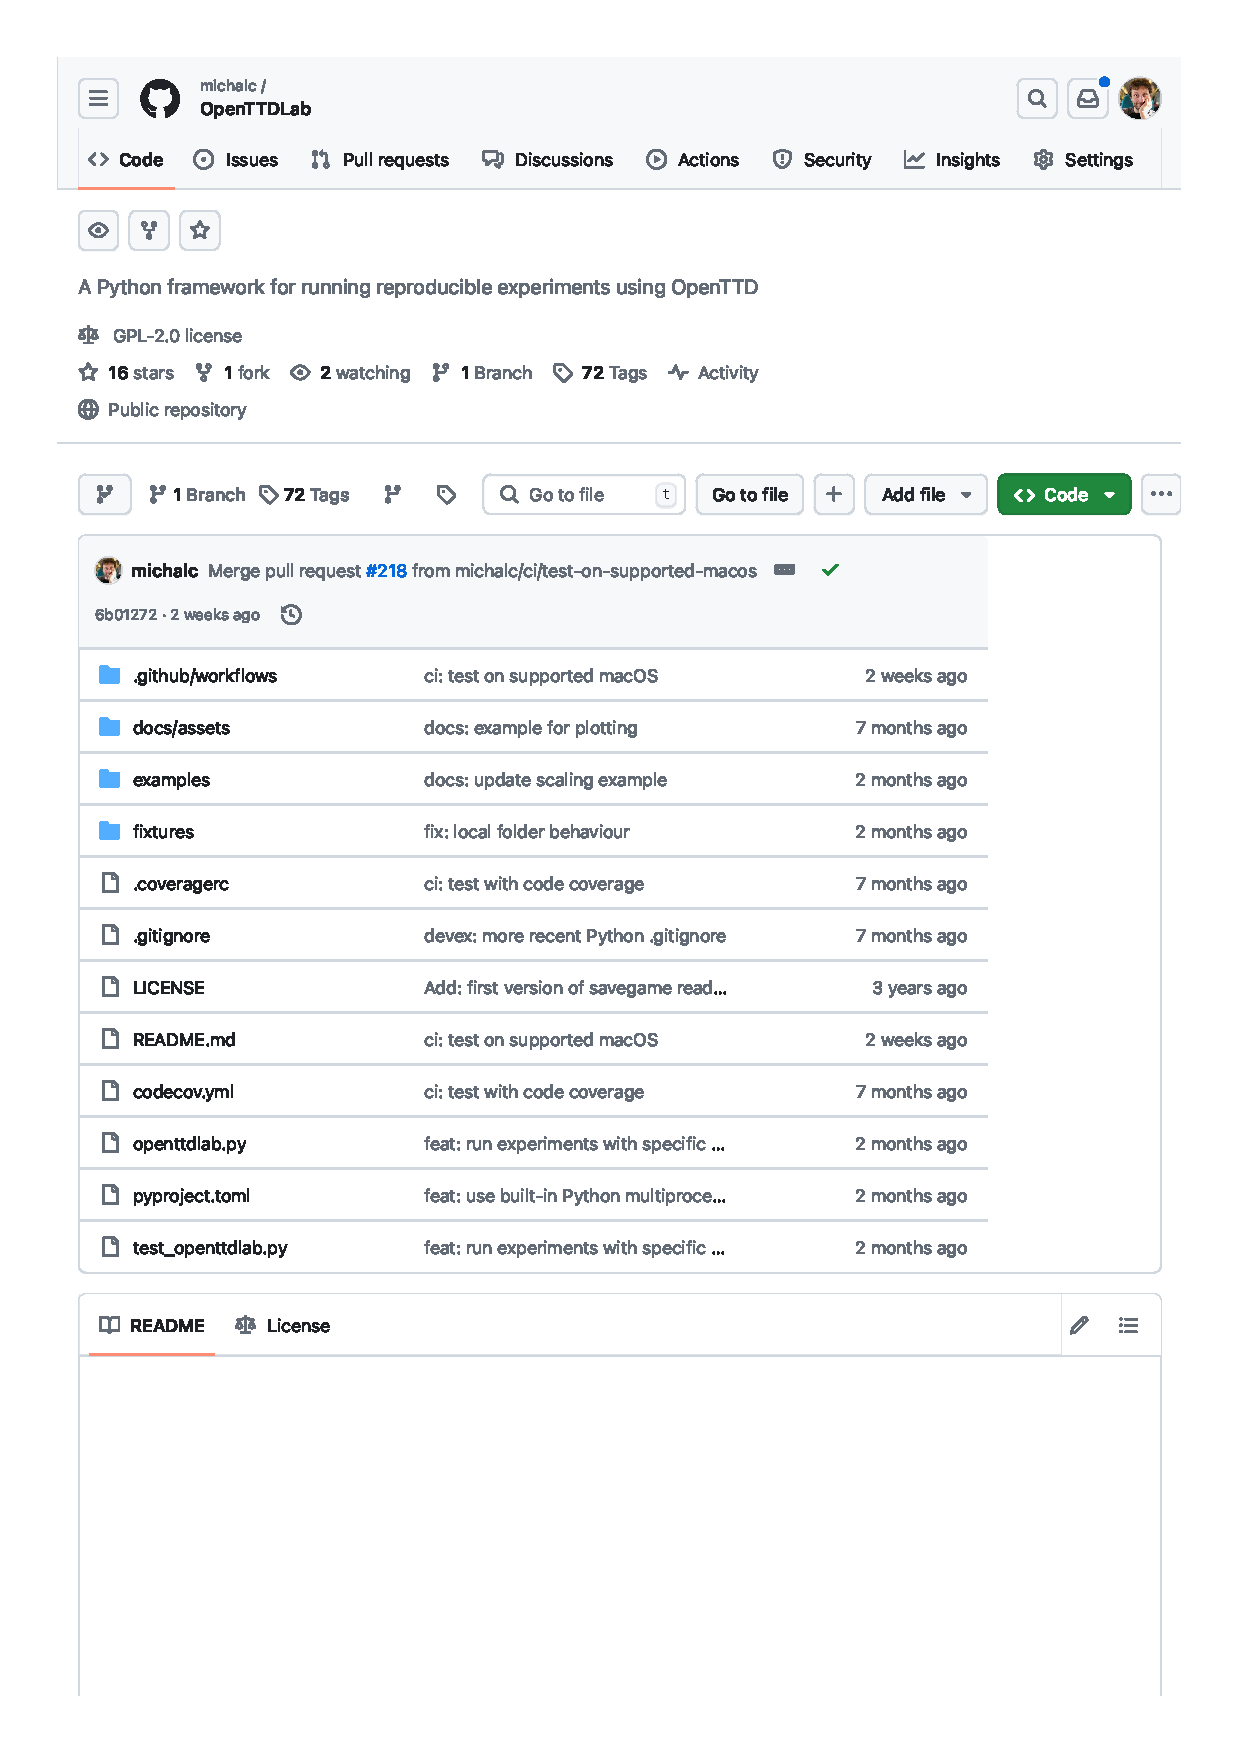
\includepdf[pages=-,width=\columnwidth,offset=0.8cm 0, pagecommand={},frame]{assets/openttdlab-github.pdf}

\chapter[Reproducing results: Python code to run experiments]{Reproducing results:\texorpdfstring{\\}{ }Python code to run experiments}
\label{chapter:trains-vs-admiral-run-experiments}

Following is a copy of Python notebook used to run the reproducing experiments of Chapter~\ref{chapter:experiments-attempt-at-reproducing}. It is available in source code form at \url{https://github.com/michalc/OpenTTDLab-MSc-Dissertation/blob/3f870c6d2f0ab77689572efdbfdf634b45edc4a7/01_trains_ai_vs_admiral_ai_01_run_experiments.ipynb}.

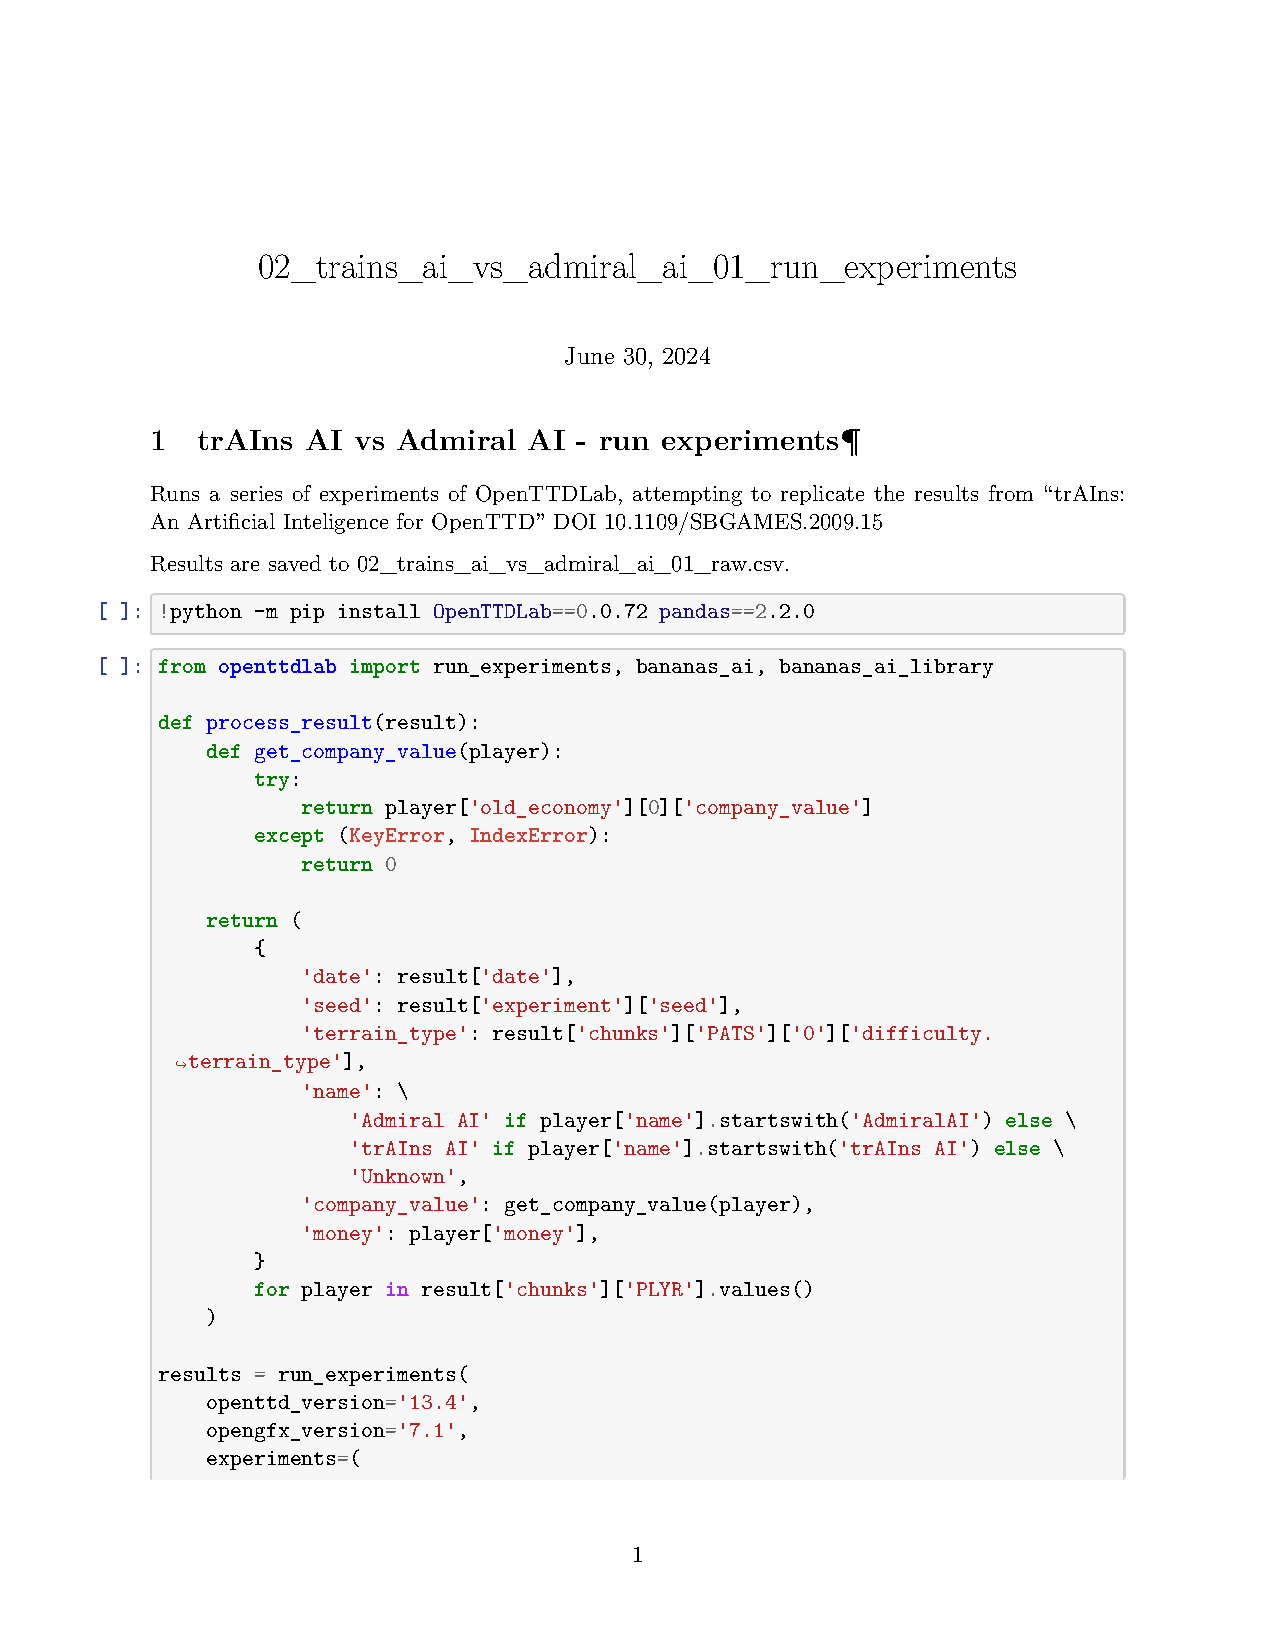
\includepdf[pages=-,width=\columnwidth,offset=0.8cm 0,pagecommand={},frame]{notebooks/01_trains_ai_vs_admiral_ai_01_run_experiments.pdf}

\chapter[Reproducing results: Python code to analyse results]{Reproducing results:\texorpdfstring{\\}{ }Python code to analyse results}
\label{chapter:trains-vs-admiral-analyse-results}

Following is a copy of the Python notebook used to analyse the results of the reproducing experiments of Chapter~\ref{chapter:experiments-attempt-at-reproducing}. It is available in source code form at \url{https://github.com/michalc/OpenTTDLab-MSc-Dissertation/blob/8d432038278685edb0988457c9d2a971a668ac64/notebooks/01_trains_ai_vs_admiral_ai_01_analyse_results.ipynb}.

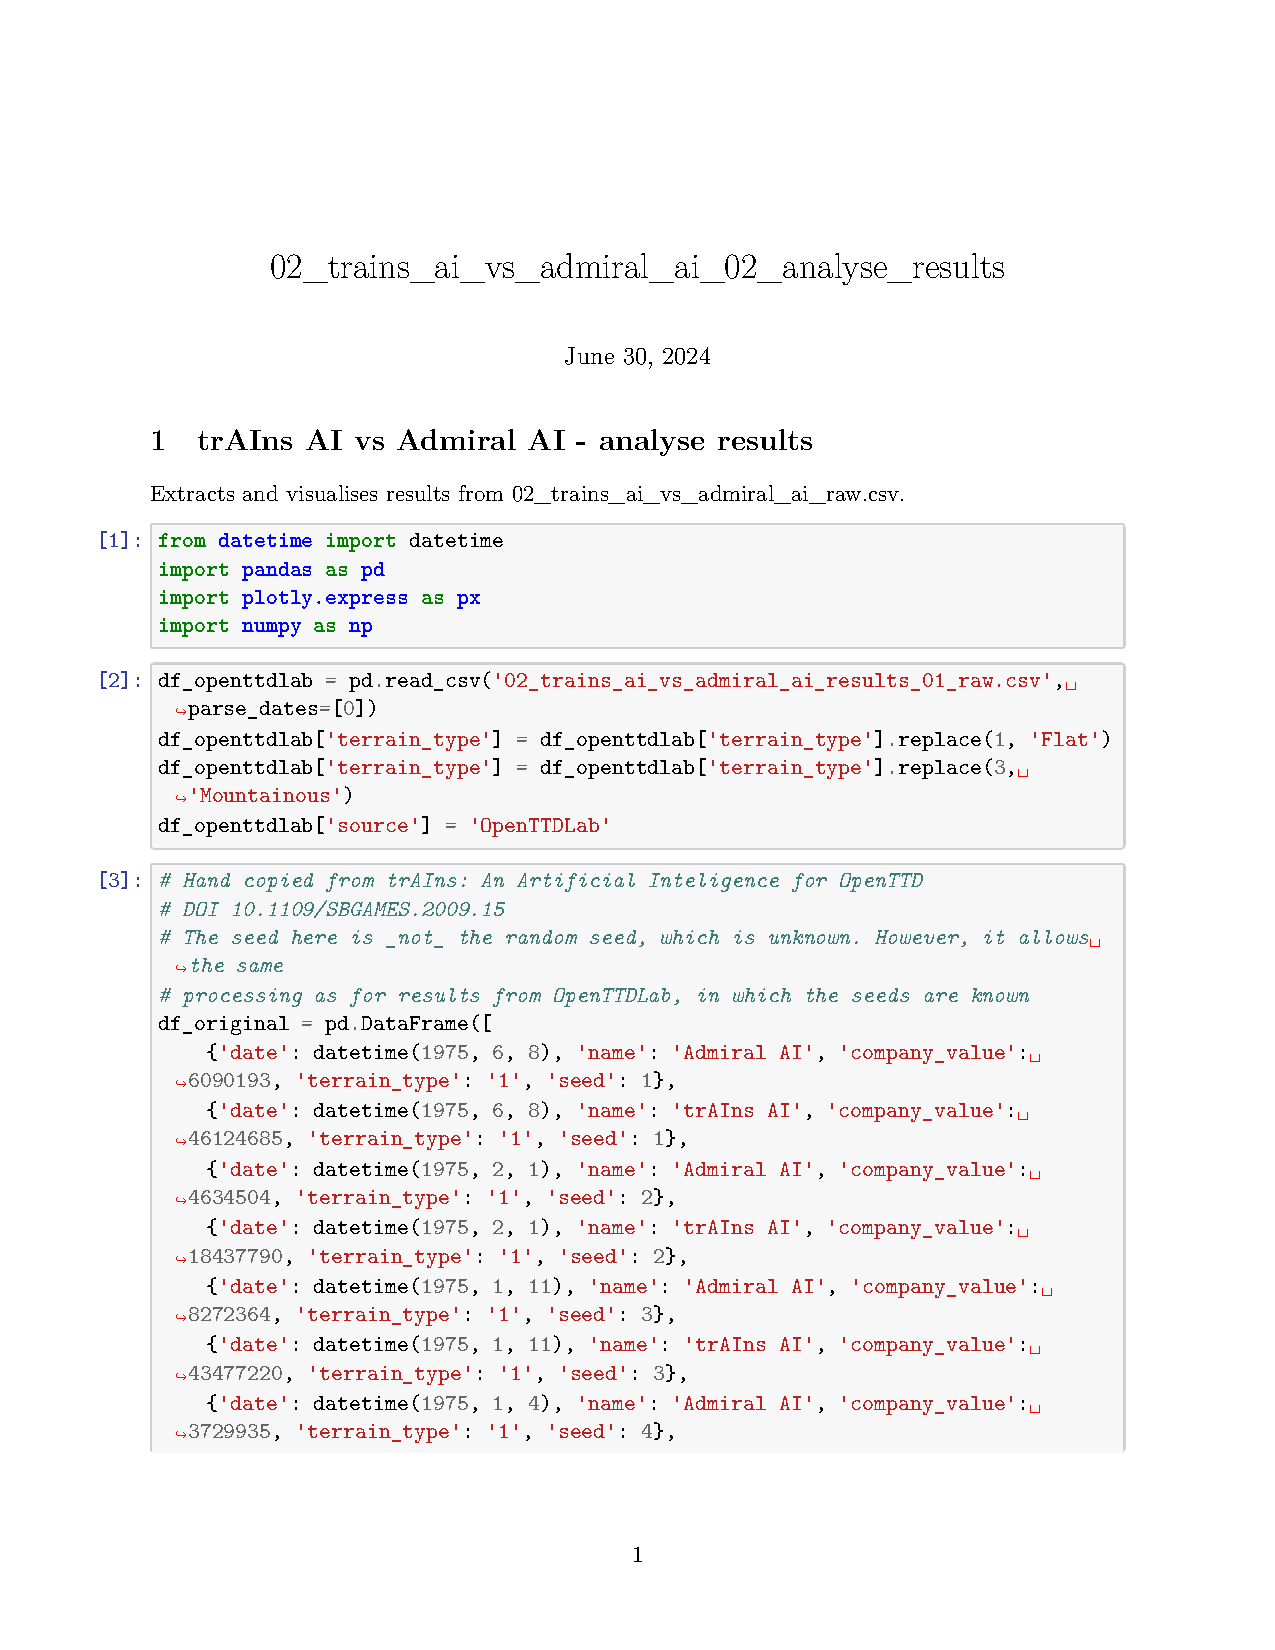
\includepdf[pages=-,width=\columnwidth,offset=0.8cm 0,pagecommand={},frame]{notebooks/01_trains_ai_vs_admiral_ai_02_analyse_results.pdf}

\chapter[Simulating a network: ParameterisedAI documentation]{Simulating a network:\texorpdfstring{\\}{ }ParameterisedAI documentation}
\label{chapter:simulating-a-network-documentation}

Following is the documentation of ParameterisedAI, the AI created for the experiments of Chapter~\ref{chapter:experiments-simple-parameterised-ai}. The copy is taken from commit \href{https://github.com/michalc/ParameterisedAI/tree/74662403e0764329112dc78e5b279d7f1b5fd510}{74662403}.

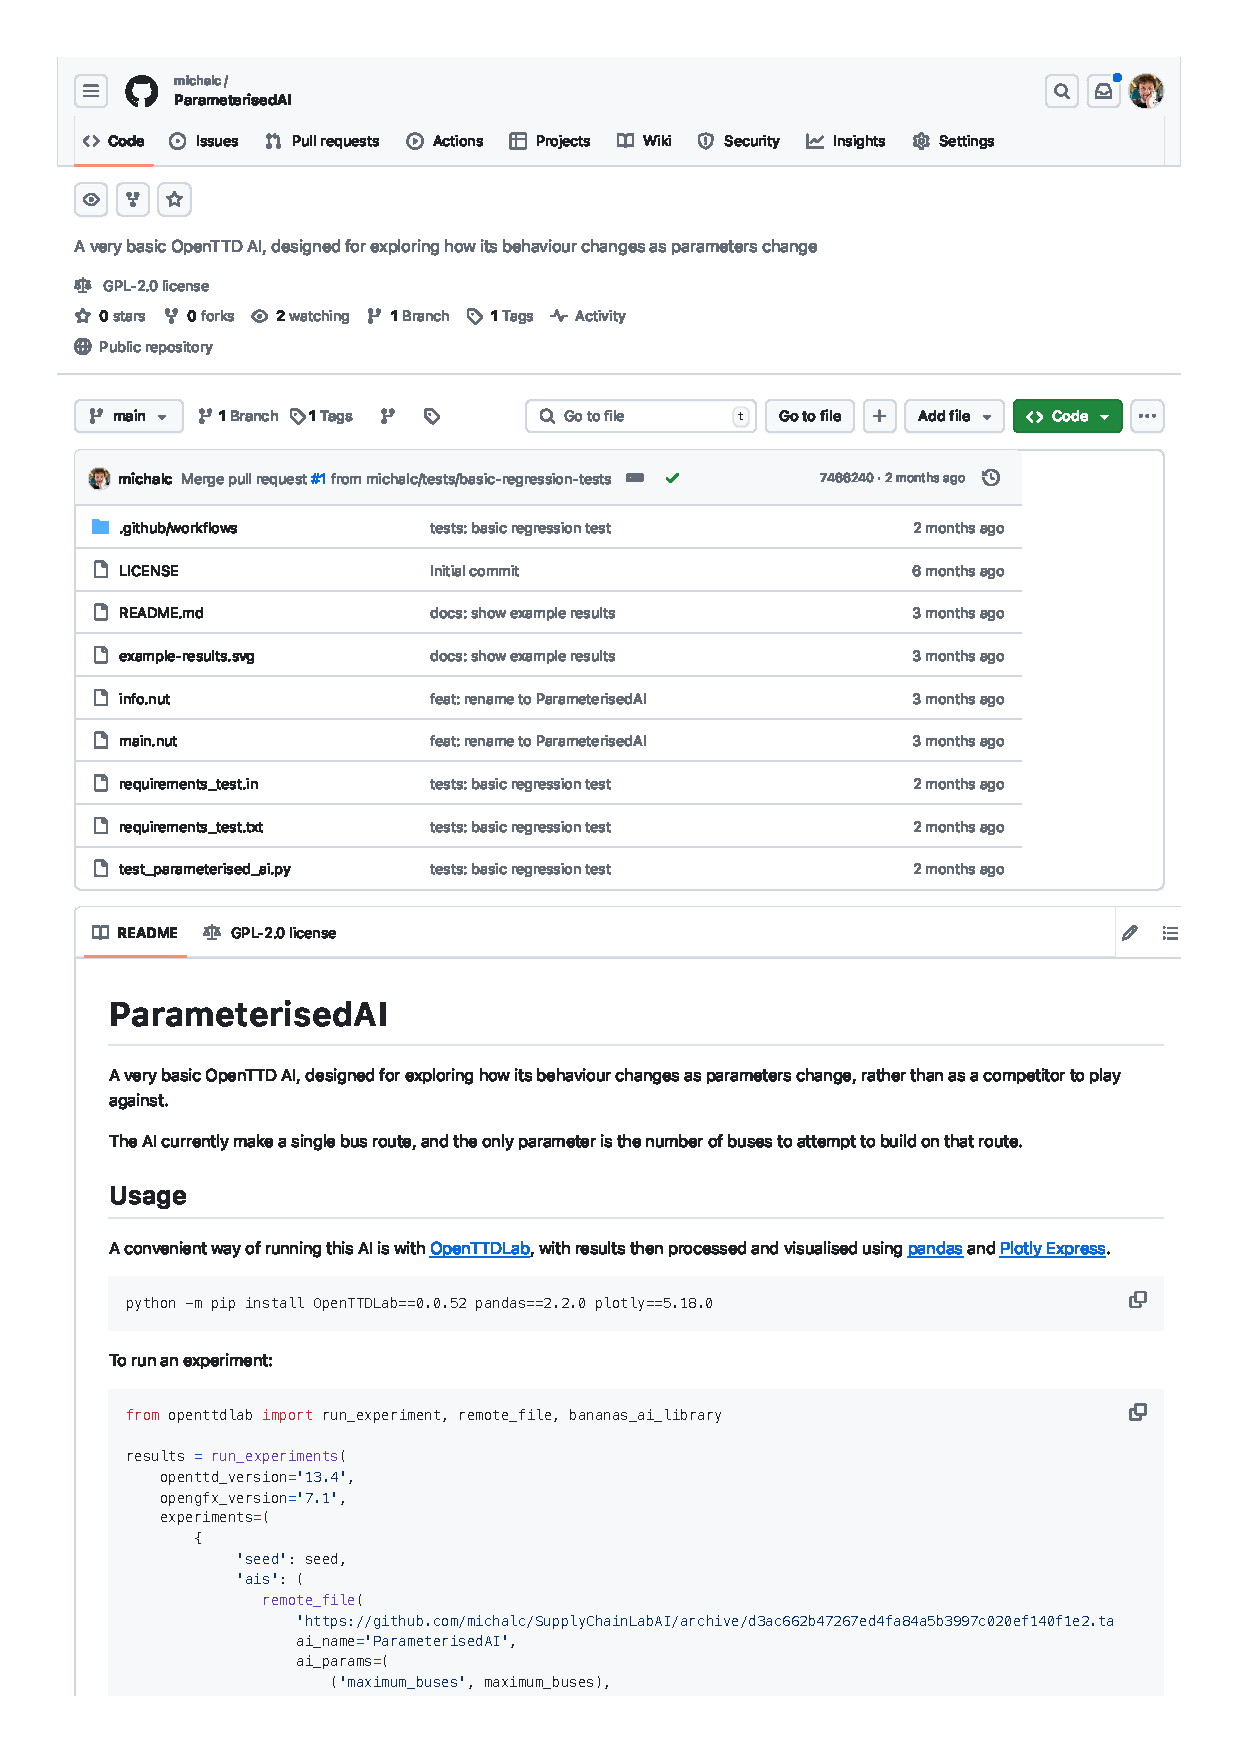
\includepdf[pages=-,width=\columnwidth,offset=0.8cm 0,pagecommand={},frame]{assets/parameterised-ai/parameterisedai-github.pdf}

\chapter[Simulating a network: ParameterisedAI Squirrel `info.nut']{Simulating a network:\texorpdfstring{\\}{ }ParameterisedAI Squirrel `info.nut'}
\label{chapter:simulating-a-network-squirrel-info}

Following is the Squirrel code of one of the two files that comprised the AI written to generate the results of Chapter~\ref{chapter:experiments-simple-parameterised-ai}, the `info.nut` file that contains the metadata of the AI. It is also available at \url{https://github.com/michalc/ParameterisedAI/blob/74662403e0764329112dc78e5b279d7f1b5fd510/info.nut}.

\lstinputlisting[language=Java]{assets/parameterised-ai/info.nut}

\chapter[Simulating a network: ParameterisedAI Squirrel `main.nut']{Simulating a network:\texorpdfstring{\\}{ }ParameterisedAI Squirrel `main.nut'}
\label{chapter:simulating-a-network-squirrel-main}

Following is the Squirrel code of one of the two files that comprised the AI written to generate the results of Chapter~\ref{chapter:experiments-simple-parameterised-ai}, the `main.nut` file that contains the core algorithm of the AI. It is also available at \url{https://github.com/michalc/ParameterisedAI/blob/74662403e0764329112dc78e5b279d7f1b5fd510/main.nut}.

\lstinputlisting[language=Java]{assets/parameterised-ai/main.nut}

\chapter[Simulating a network: ParameterisedAI Python regression test]{Simulating a network:\texorpdfstring{\\}{ }ParameterisedAI Python regression test}
\label{chapter:simulating-a-network-python-regression-test}

Following is the Python regression test of the AI written to generate the results of Chapter~\ref{chapter:experiments-simple-parameterised-ai}. It is also available at \url{https://github.com/michalc/ParameterisedAI/blob/74662403e0764329112dc78e5b279d7f1b5fd510/test_parameterised_ai.py}.

\lstinputlisting[language=Python]{assets/parameterised-ai/test_parameterised_ai.py}

\chapter[Simulating a network: Python code to run experiments]{Simulating a network:\texorpdfstring{\\}{ }Python code to run experiments}
\label{chapter:own-parameterised-ai-run-experiments}

Following is a copy of Python notebook used to run the network simulation experiments of Chapter~\ref{chapter:experiments-simple-parameterised-ai}. It is available in source code form at \url{https://github.com/michalc/OpenTTDLab-MSc-Dissertation/blob/8d432038278685edb0988457c9d2a971a668ac64/notebooks/02_own_parameterised_ai_01_run_experiments.ipynb}.

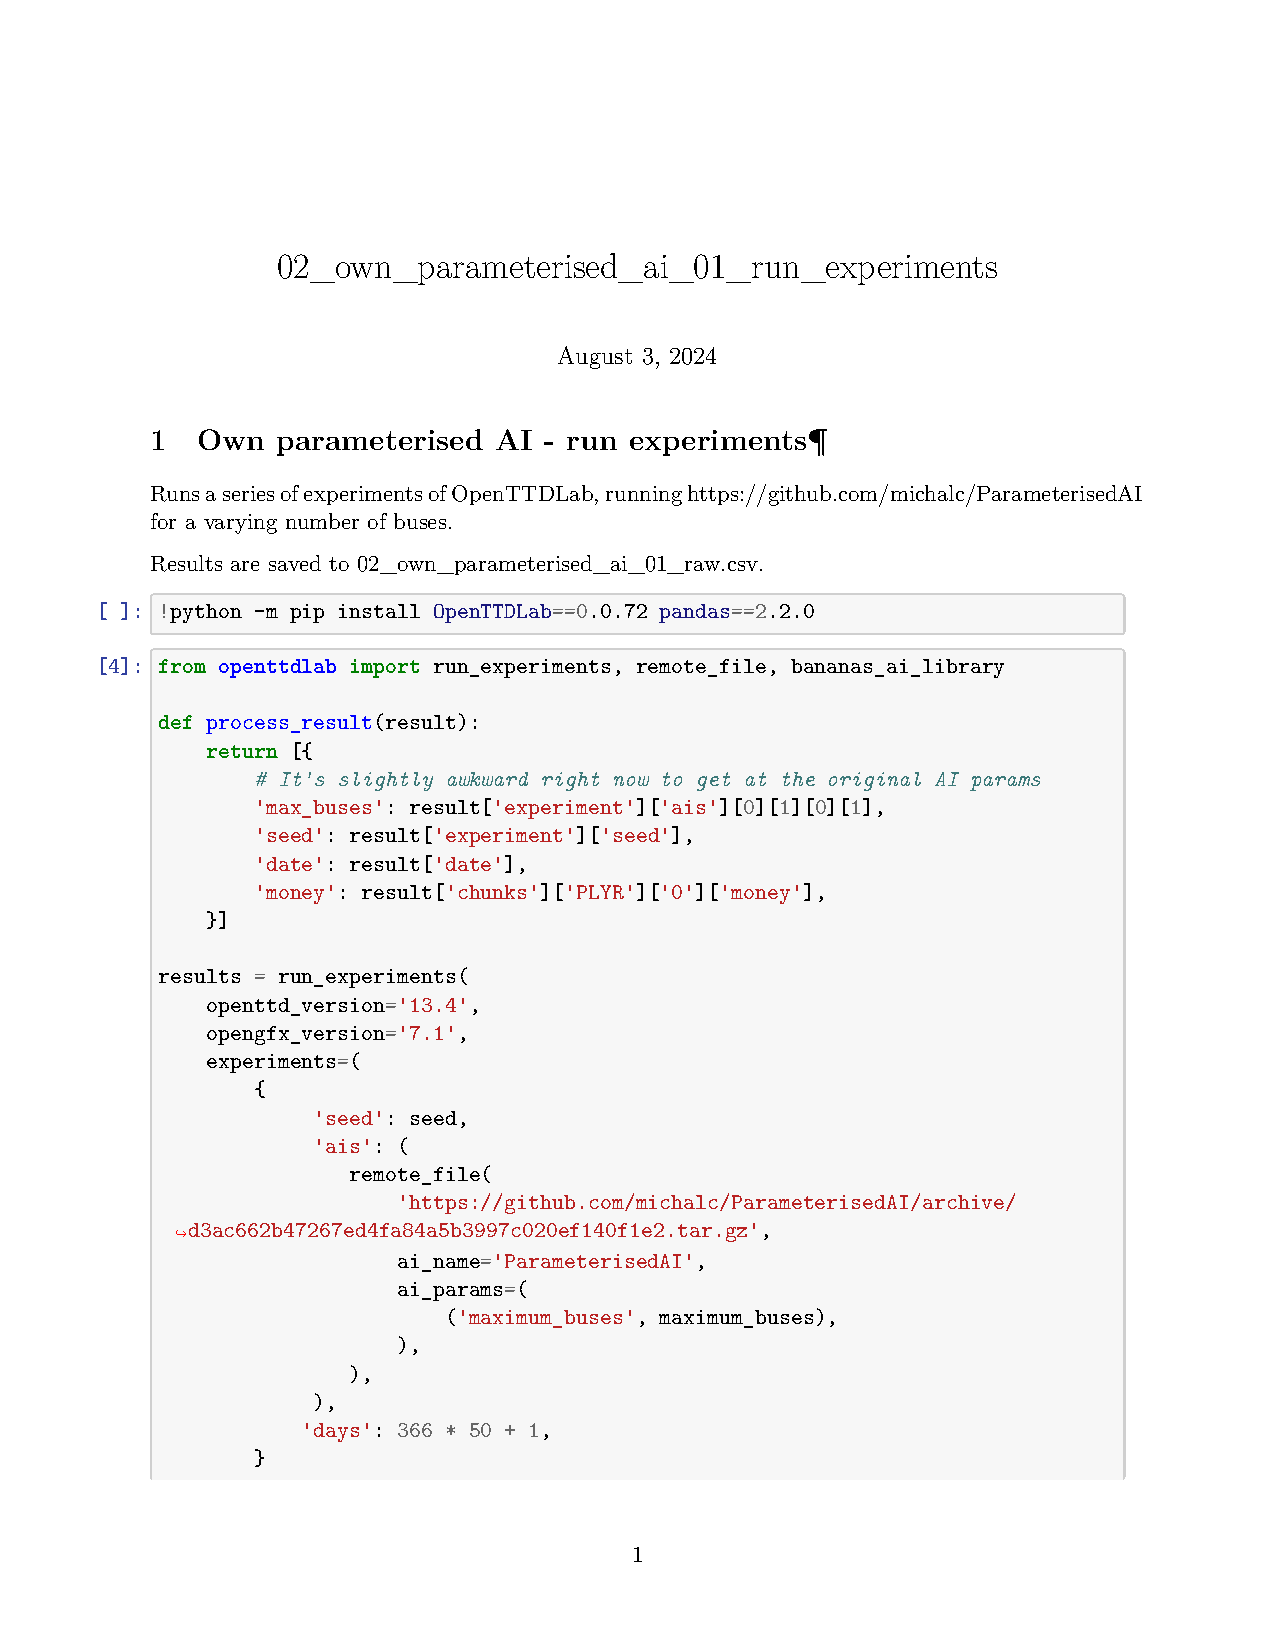
\includepdf[pages=-,width=\columnwidth,offset=0.8cm 0,pagecommand={},frame]{notebooks/02_own_parameterised_ai_01_run_experiments.pdf}

\chapter[Simulating a network: Python code to analyse results]{Simulating a network:\texorpdfstring{\\}{ }Python code to analyse results}
\label{chapter:own-parameterised-ai-analyse-results}

Following is a copy of Python notebook used to analyse results of the network simulation experiments of Chapter~\ref{chapter:experiments-simple-parameterised-ai}. It is available in source code form at \url{https://github.com/michalc/OpenTTDLab-MSc-Dissertation/blob/8d432038278685edb0988457c9d2a971a668ac64/notebooks/notebooks/02_own_parameterised_ai_02_analyse_results.ipynb}.

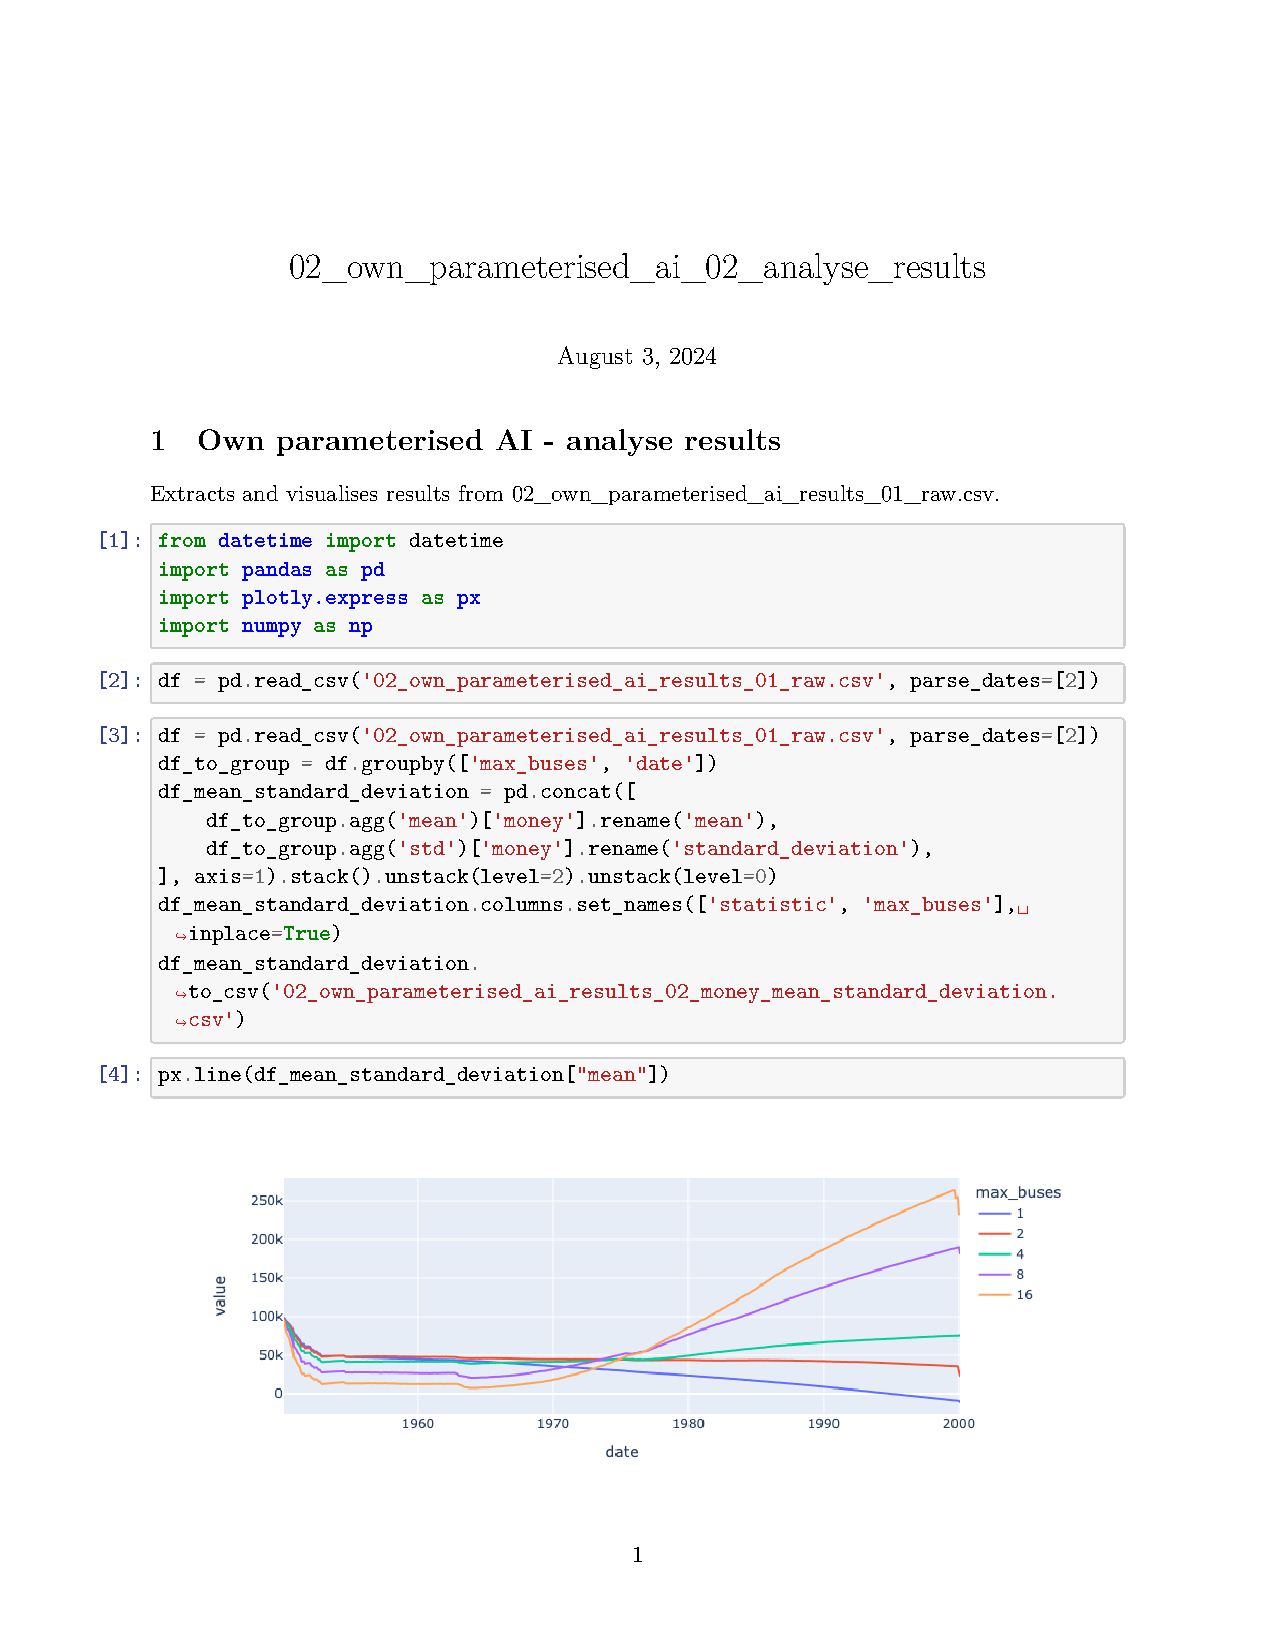
\includepdf[pages=1-1,width=\columnwidth,offset=0.8cm 0,pagecommand={},frame]{notebooks/02_own_parameterised_ai_02_analyse_results.pdf}

\chapter[Scaling: Python code to run experiments]{Scaling:\texorpdfstring{\\}{ }Python code to run experiments}
\label{chapter:scaling-running-code}

Following is a copy of Python notebook used to run the scaling experiments of Chapter~\ref{chapter:experiments-scaling}. It is available in source code form at \url{https://github.com/michalc/OpenTTDLab-MSc-Dissertation/blob/8d432038278685edb0988457c9d2a971a668ac64/notebooks/03_scaling_01_run_experiment.ipynb}.

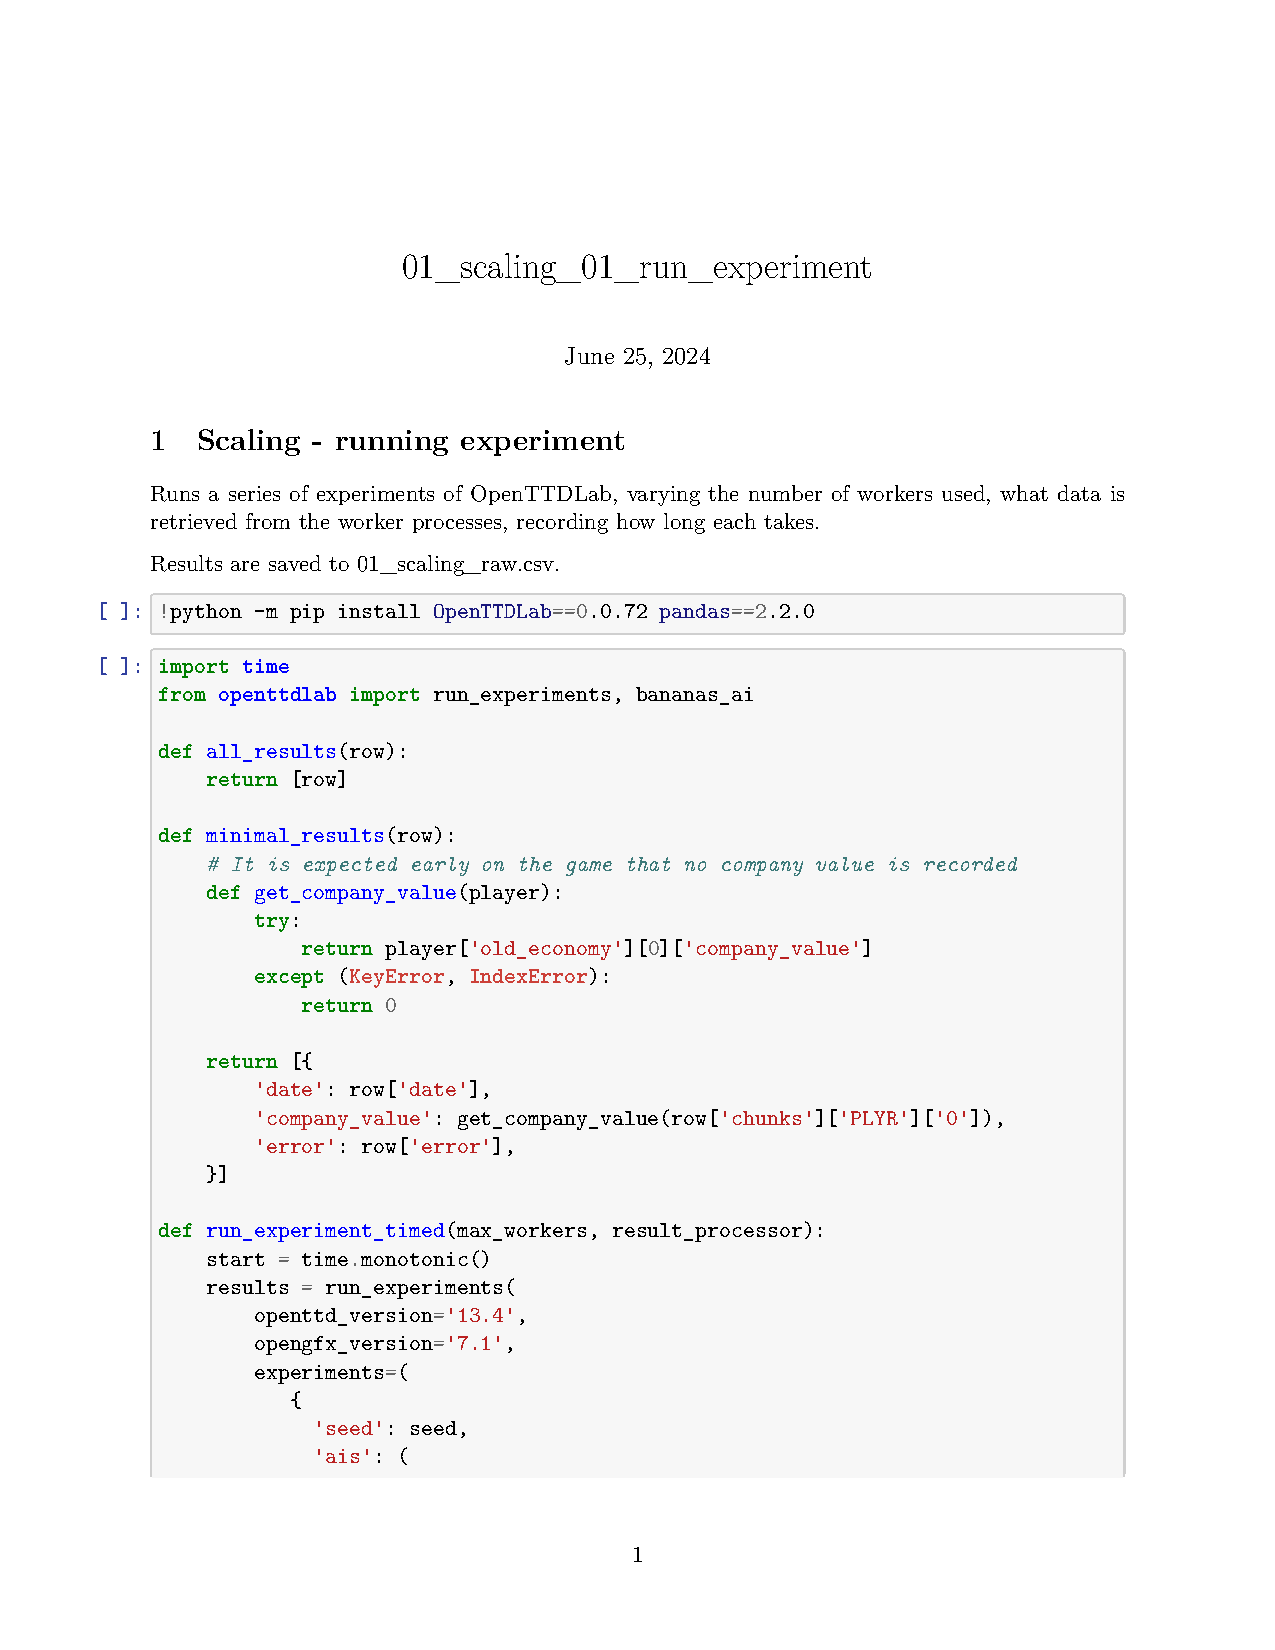
\includepdf[pages=-,width=\columnwidth,offset=0.8cm 0,pagecommand={},frame]{notebooks/03_scaling_01_run_experiment.pdf}

\chapter[Scaling: Python code to analyse results]{Scaling:\texorpdfstring{\\}{ }Python code to analyse results}

\label{chapter:scaling-analyis-code}

Following is a copy of Python notebook used to analyse results of the scaling experiments of Chapter~\ref{chapter:experiments-scaling}. It is available in source code form at \url{https://github.com/michalc/OpenTTDLab-MSc-Dissertation/blob/8d432038278685edb0988457c9d2a971a668ac64/notebooks/03_scaling_02_analyse_results.ipynb}

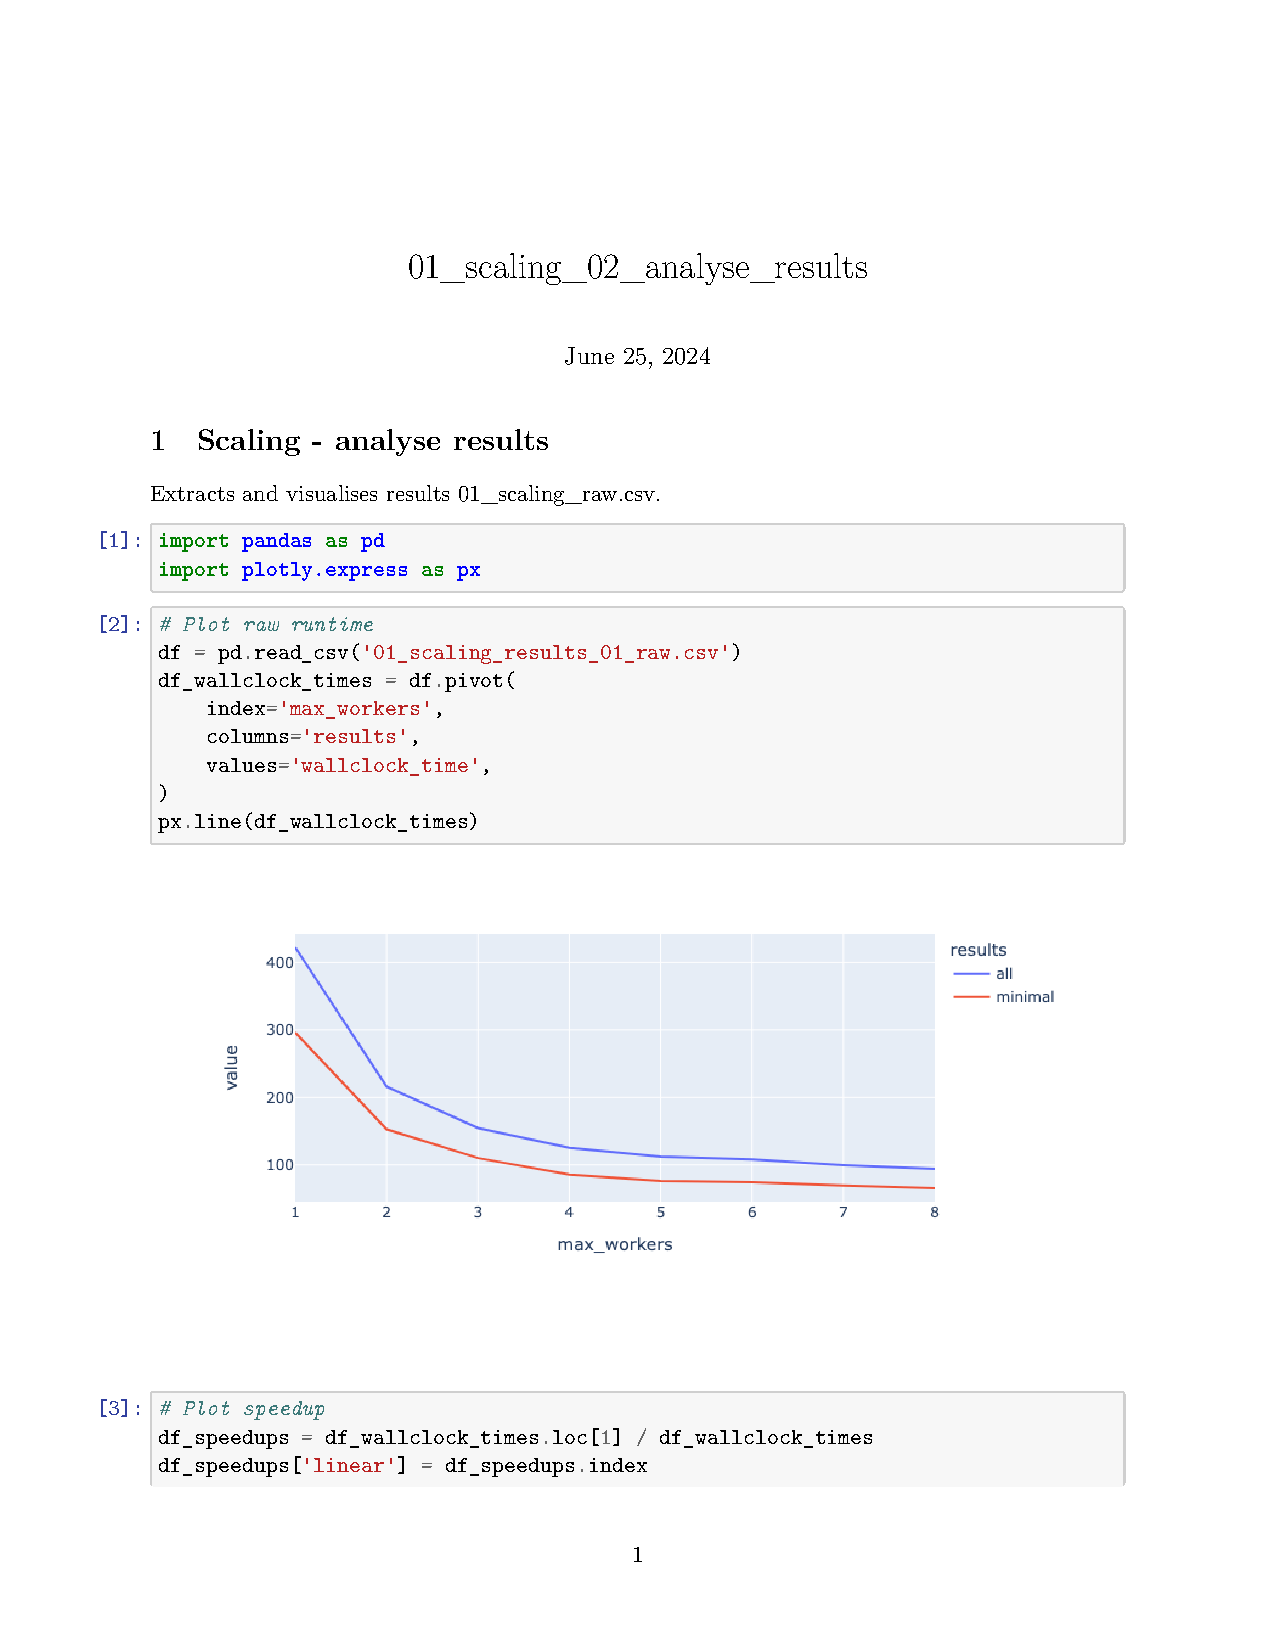
\includepdf[pages=-,width=\columnwidth,offset=0.8cm 0,pagecommand={},frame]{notebooks/03_scaling_02_analyse_results.pdf}

\end{document}
